\documentclass[whitelogo]{tudelft-report}
\usepackage{natbib}
\usepackage{changes}
\usepackage{todonotes}
\usepackage{tabularx}
\usepackage{listings}
\begin{document}

%% Use Roman numerals for the page numbers of the title pages and table of
%% contents.
\frontmatter

%% Uncomment following 19 lines for a cover with a picture on the lower half only
\title[tudelft-white]{Identifying and Managing Technical Debt in Complex Distributed Systems}
%\subtitle[tudelft-cyan]{Optional subtitle}
\author[tudelft-white]{M.A. de Vos}
\affiliation{Technische Universiteit Delft}
%\coverimage{cover.jpg}
%\titleoffsetx{10cm}
%\titleoffsety{10cm}
%\afiloffsetx{1cm}
%\afiloffsety{18cm}
%\covertext[tudelft-white]{
%    \textbf{Cover Text} \\
%    possibly \\
%    spanning 
%    multiple 
%    lines
%    \vfill
%    ISBN 000-00-0000-000-0
%}
%\makecover

%% Uncomment following 16 lines for a cover with a picture on the lower half only
%\title[tudelft-white]{}
%\subtitle[tudelft-black]{Optional subtitle}
%\author[tudelft-white]{J.\ Random Author}
%\affiliation{Technische Universiteit Delft}
%\coverimage{tank.jpg}
%\covertext[tudelft-white]{
%    \textbf{Cover Text} \\
 %   possibly \\
  %  spanning 
%    multiple 
%    lines
%    \vfill
%    ISBN 000-00-0000-000-0
%}
%\setpagecolor{tudelft-cyan}
%\makecover[split]
\setlength\parindent{0pt}

%% Include an optional title page.
\begin{titlepage}


\begin{center}

%% Insert the TU Delft logo at the bottom of the page.

%% Print the title in cyan.
{\makeatletter
\largetitlestyle\fontsize{64}{94}\selectfont\@title
%\largetitlestyle\color{tudelft-cyan}\Huge\@title
\makeatother}

%% Print the optional subtitle in black.
{\makeatletter
\ifx\@subtitle\undefined\else
    \bigskip
   {\tudsffamily\fontsize{22}{32}\selectfont\@subtitle}    
    %\titlefont\titleshape\LARGE\@subtitle
\fi
\makeatother}

\bigskip
\bigskip

by
%door

\bigskip
\bigskip

%% Print the name of the author.
{\makeatletter
%\largetitlefont\Large\bfseries\@author
\largetitlestyle\fontsize{26}{26}\selectfont\@author
\makeatother}

\bigskip
\bigskip

to obtain the degree of Master of Science
%ter verkrijging van de graad van Master of Science

at the Delft University of Technology,
%aan de Technische Universiteit Delft,

to be defended publicly on Tuesday January 1, 2013 at 10:00 AM.
%in het openbaar de verdedigen op dinsdag 1 januari om 10:00 uur.

\vfill

\begin{tabular}{lll}
    Student number: & 1234567 \\
    Project duration: & \multicolumn{2}{l}{March 1, 2012 -- January 1, 2013} \\
    Thesis committee: & Prof.\ dr.\ ir.\ J.\ Doe, & TU Delft, supervisor \\
        & Dr.\ E.\ L.\ Brown, & TU Delft \\
        & Ir.\ A.\ Aaronson, & Acme Corporation
\end{tabular}
%% Only include the following lines if confidentiality is applicable.

\bigskip
\bigskip
\emph{This thesis is confidential and cannot be made public until December 31, 2013.}
%\emph{Op dit verslag is geheimhouding van toepassing tot en met 31 december 2013.}

\bigskip
\bigskip
An electronic version of this thesis is available at \url{http://repository.tudelft.nl/}.
%\\[1cm]

%\centering{
\includegraphics{cover/logo_black}}


\end{center}

\begin{tikzpicture}[remember picture, overlay]
    \node at (current page.south)[anchor=south,inner sep=0pt]{
        
\includegraphics{cover/logo_black}
    };
\end{tikzpicture}

\end{titlepage}



\chapter*{Abstract}
The term \emph{technical debt} has been used to described the increased cost of changing or maintaining a system due to expedient shortcuts taken during development, possibly due to budget or time constraints. The term has gained significant attention in the agile and academic community and several models have been proposed to keep track of and solve technical debt.\\\\
Tribler, a decentralized platform to share and discover content in a complete decentralized way, has accumulated a tremendous amount of technical debt over the last ten years of scientific research in the area of peer-to-peer networking. This thesis will focus on disruptive improvements to the architecture, user interface and testing framework of Tribler. With the deletion of 12.581 lines, the modification of 765 lines and addition of 12.429 lines, we show that various important software metrics are improved.\\\\
Our performance experiments will demonstrate that the performance of Tribler has not significantly degraded due to the invasive modifications\todo{verbeteren}.
\chapter*{Preface}
\setheader{Preface}

Preface\ldots

\begin{flushright}
{\makeatletter\itshape
    \@author \\
    Delft, January 2013
\makeatother}
\end{flushright}



\tableofcontents

%% Use Arabic numerals for the page numbers of the chapters.
\mainmatter

\chapter{Introduction}

% Software aging: https://www.cs.drexel.edu/~yfcai/CS451/RequiredReadings/SoftwareAging.pdf
% Measuring and Monitoring Technical Debt http://ccsl.org.br/files/TD%20talk%20USP.pdf

The resources, budget and time frame of software engineering projects are often constrained.
This requires software engineers to analyse trade-offs that have to be made in order to meet deadlines and budgets.
Making decisions that are beneficial on the short term, might lead to significantly increased maintenance costs in the long run.
The phenomenon of favouring short-term development goals over longer term requirements is often referred to as \emph{technical debt}.
While technical debt might not have implicit consequences on the user experience, it dramatically impacts quality and maintainability of the software.\\\\
The term technical debt was first introduced by Ward Cunningham as writing "not quite right" code in order to ship a new product or feature to market faster\cite{cunningham1993wycash}.
Since then, the term has gained progressively more attention in the software engineering research and the agile community.
Effective management of such debt is considered critical to achieve and maintain a high level of software quality.
In 2007, Steve McConnell created the technical debt taxonomy where he refined and expanded the definition\cite{mcconnell2007debt}.
He points out that some kind of engineering practices are not considered technical debt, such as deferred features, incomplete work that is not shipped and other features where one does not have to 'pay' debt for.
Martin Fowler considers technical debt more as a metaphor to use when communicating with non-technical people and introduced the technical debt quadrant in 2009\cite{technicaldebtquadrant}.
According to his work, technical debt can be categorized in distinct types, separating issues arising from recklessness from those decisions that are made strategically. 
Figure \ref{fig:technical-debt-quadrant} presents this distinction in more detail.\\

\begin{figure}[!h]
	\centering
	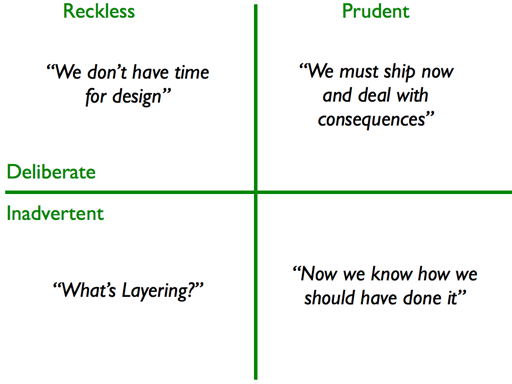
\includegraphics[width=0.5\columnwidth]{images/technical_debt_quadrant}
	\caption{The technical debt quadrant, as proposed by Martin Fowler.}
	\label{fig:technical-debt-quadrant}
\end{figure}

Technical debt can be both invisible and visible to end users\cite{kruchten2012technical}.
Examples of invisible technical debt includes code smells, coding style violations, low internal quality and high code complexity.
Visible technical debt is expressed in bugs that are affecting users but can also be identified by user-unfriendly, cluttered graphical user interfaces.
Decisions to extend and evolve the graphical user interface with new visual elements, can lead to a high amount of technical debt and a poor user experience.\\\\
The term itself is borrowed from the finance domain\cite{guo2011portfolio}.
There is however one important distinction between financial debt and technical debt.
When working with financial debt, the costs that the debtor has to pay is usually clear.
This is not always the case with technical debt: there might be some situations where no technical debt incurred.
For instance, if it is known for a part of the system to never be updated or maintained in the future, time can be saved by not updating the related documentation.
Software engineers have to carefully consider what technical debt they wish to incur and when this debt will be paid off.\\\\
There are several causes that contribute to the amount of accumulated technical debt during the software development process\cite{martini2014architecture}. While notable to a lesser extent in research-oriented software engineering, time pressure can cause developers to think reckless about their architecture. Uncertainty in  decision making during an early stage of development might lead to higher technical debt. Finally, in an agile environment, software requirements might change more often, causing the underlying architecture and code base to change. Not properly managing such changes can lead to significant technical debt.\\\\
Tribler is the result of 10 ongoing years of scientific research in the field of decentralized network technology and has incurred a serious amount of technical debt, both visible and invisible for users.
The software allows users to discover and download interesting content such as music and videos in a completely decentralized manner.
In 2014, support for anonymous download using a Tor-like protocol has been added by the work of R. Plak\cite{plak2014anonymous} and J.H. Tanaskoski\cite{tanaskoski2014anonymous}. 
In 2015, the protocol has been extended to support for anonymous seeding of torrents\cite{ruigrok2015bittorrent}.
The graphical user interface of Tribler is shown in figure \ref{fig:tribler-interface}.

\begin{figure}[!h]
	\centering
	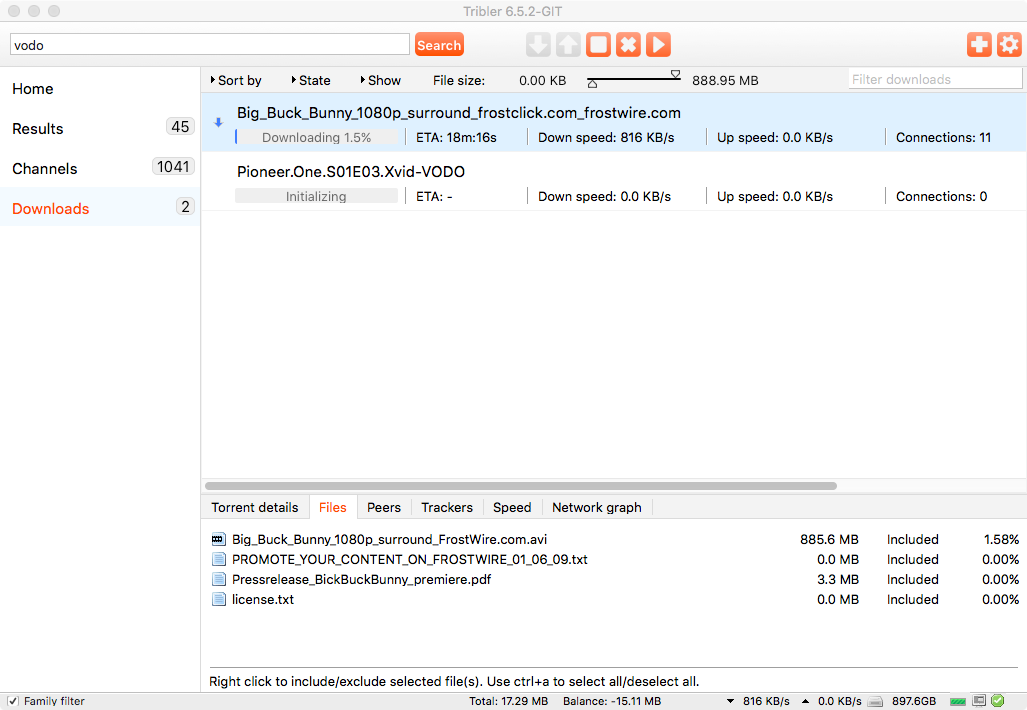
\includegraphics[width=0.9\columnwidth]{images/tribler_interface}
	\caption{The graphical user interface of Tribler v6.5.2.}
	\label{fig:tribler-interface}
\end{figure}

\newpage

The focus of this thesis will be tracking and managing technical debt in Tribler. The following research question can be formulated:\\\\
\emph{How can we track and manage technical debt within Tribler?}\\\\
This question can be divided into some subquestions:
\begin{enumerate}
	\item What tools should be used to identity technical debt within Tribler?
	\item What kind of technical debt should be prioritized for fixing?
	\item What are the adequate requirements in the software development process to make the right decisions about incurring technical debt in the future?
\end{enumerate}

The rest of this document is outlined as follows: in Chapter \ref{chapter:problem-description}, the current state of the system will be elaborated, highlighting flaws and impurity in the architecture and code base. 
In Chapter \ref{chapter:architecture}, the evolution of Tribler over the past 10 years will be presented and we build foundations for the next decade of scientific research with Tribler by proposing a new future-proof and robust architecture.
Various efforts to improve quality assurance, code quality and infrastructure while paying off technical debt will be explained in Chapter \ref{chapter:refactoring}.
The performance of Tribler after refactoring efforts will be discussed in Chapter \ref{chapter:experiments}.
By conduction various benchmarks and performance measurements, the user experience of Tribler will be assessed.
We will end with the conclusions and propose future work in Chapter \ref{chapter:conclusions}.

\chapter{Problem Description}
\label{chapter:problem-description}
The goal of this thesis project is to help Tribler mature from an experimental research prototype into production-level code with reliable usage by millions of users.\\\\
After careful analysis it was decided that within the context of a nine month project the strongest contribution to the future of Tribler would be a reduction in technical debt. At this point we believe the project does not need a particular focus on feature improvements, novel additional features, or boosting performance. After more than ten years of software development by 44 unique contributors the amount of accumulated technical debt is worrying.\\\\
Tribler suffers from all kinds of technical debt, including instability issues, race conditions, coding style violations, code complexity, deferred infrastructure update decisions and feature pollution in the graphical user interface. This is illustrated by the fact that there even is a dedicated file in the Tribler code base, called \emph{hacks.py} that facilitates various workarounds caused by incompatible software.\\\\
This thesis is focussed on a round of invasive maintenance and cleaning of the code and all other infrastructure such as the continuous integration environment and installers. Our work aims to ensure that it is possible to conduct another decade of experimental distributed systems research with the Tribler code base. The alternative is continued usage and expansion of the code, which is likely to lead to a forced clean slate approach.\\\\
The structural problem is the lack of maintenance capacity. Each contributor to the Tribler research in the form of a bachelor, master, or PhD student needs to be primarily focussed on their thesis work. A thesis requires concrete experimental results, contribution to theory, or both. We believe that the lack of student enthusiasm for fixing bugs, writing documentation and the absence of a code review policy are the root causes of current state of the code base.\\\\
In this remaining of this Chapter, various problems within the Tribler project will be highlighted and discussed.

\section{A large code base}
Tribler consists of a large and complex code base. This makes Tribler an unattractive open-source project for external developers to work on since the process to get familiar with the code base takes a considerably amount of time. Figure \ref{fig:openhub-commits} illustrates the number of commits per months over the past ten years of Tribler software engineering. The evolution of the amount of source lines of code (SLOC) is shown in Figure \ref{fig:openhub-loc}. The magnitude of the project is also presented by Figure \ref{fig:openhub-commit-stats}. From these Figures, it becomes evident that Tribler has continued to grow to a project with an unmaintainable amount of code. According to the basic software cost estimation model COCOMO\cite{kemerer1987empirical}, the established costs of the project is \$2,371,403 with an estimated effort of 43 person-years.\\\\
This continued growth can be explained by the fact that Tribler is a research-oriented prototype. Students often contribute to Tribler by implementing a specific feature of the system, such as a anonymous download mechanism, a credit mining system or an adult filter to hide explicit content in the user interface. After delivery of these features, the student leaves the project and knowledge about that specific part of Tribler he or she contributed to, is lost. Afterwards, that part of Tribler transits to an unmaintained state, due to lack of knowledge and manpower.\\\\
Continuous expansion of a system inevitably leads to feature pollution. During the lifetime of Tribler, no single effort has been made to do a proper clean up of the code, leading to a huge amount of technical debt. If this trend continues, Tribler will evolve into an tremendously complex system where the choice to use a clean-slate approach is favoured over continued usage of the current code base, leading to much wasted development effort.

\begin{figure}[!h]
	\centering
	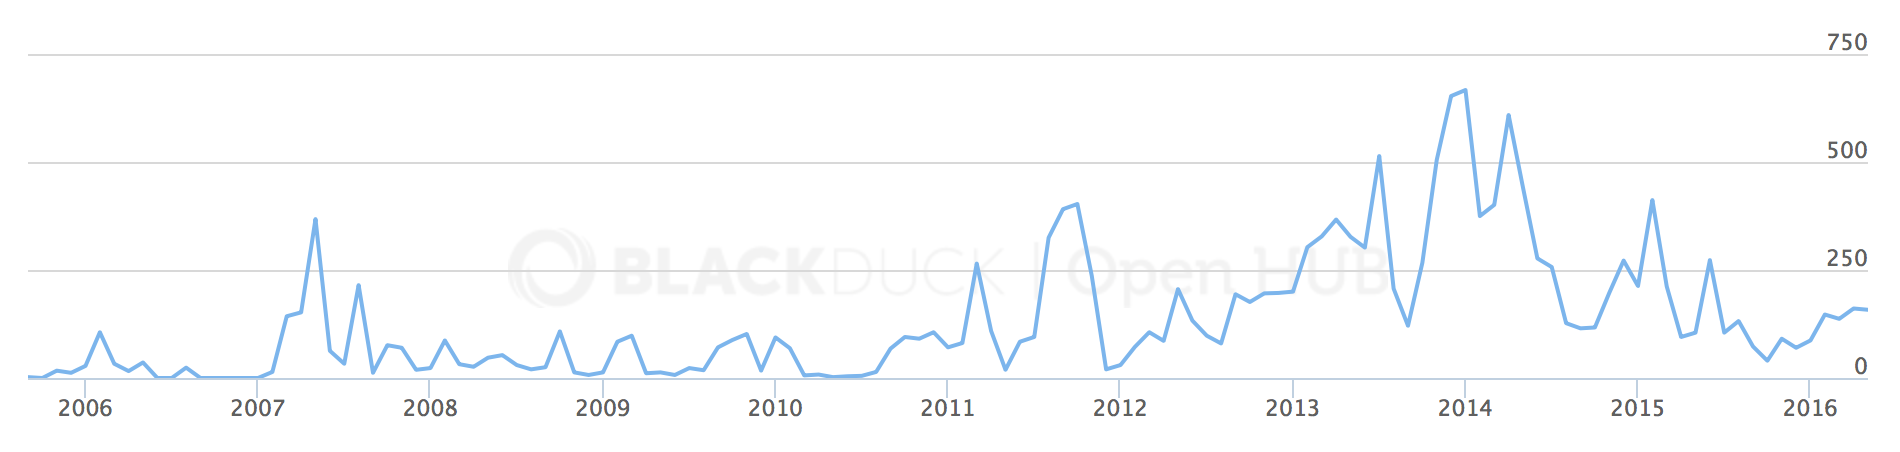
\includegraphics[width=\columnwidth]{images/problem_description/openhub_commits}
	\caption{A history of commits per month on the Tribler project, as reported by Open Hub.}
	\label{fig:openhub-commits}
\end{figure}

\begin{figure}[!h]
	\centering
	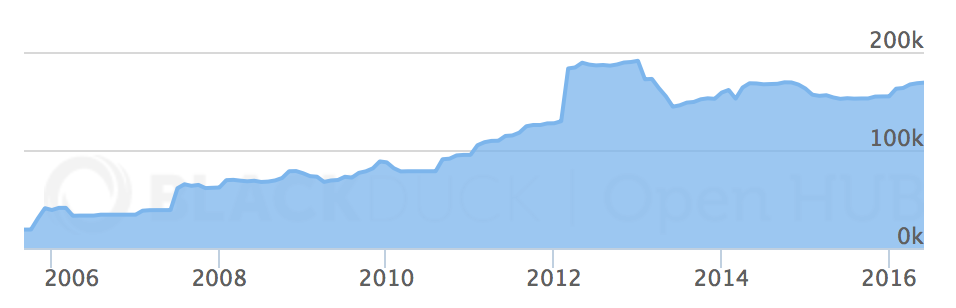
\includegraphics[width=\columnwidth]{images/openhub_loc}
	\caption{The evolution of lines of code in the Tribler project, as reported by Open Hub.}
	\label{fig:openhub-loc}
\end{figure}

\begin{figure}[!h]
	\centering
	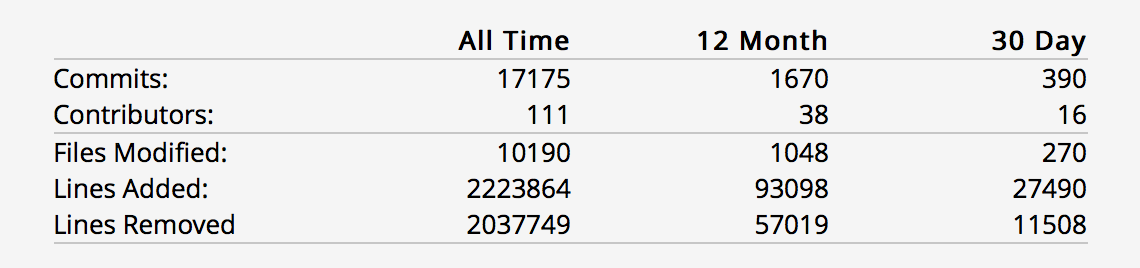
\includegraphics[width=0.7\columnwidth]{images/openhub_commits_table}
	\caption{Statistics about modifications to the code base, as reported by Open Hub.}
	\label{fig:openhub-commit-stats}
\end{figure}

\section{Lack of Maintenance}
Many features of Tribler are completely unmaintained, due to lack of knowledge or resource constraints. There are even some experimental features that are enabled due to malfunctioning which could be removed.\\\\
The lack of maintenance is clearly visible in the messaging system of Tribler, called \emph{Dispersy}. Dispersy is a platform to simplify the design of decentralized communities and is mostly designed and written by
N. Zeilemaker and B. Schoon\cite{zeilemaker2013dispersy}. After these developers left the project, knowledge of the Dispersy system disappeared and the system transited to an unmaintained state where the process of fixing new defects is being deferred.\\\\
Most researchers contributing to Tribler have a specific feature to deliver. This means that defects in unmaintained parts of Tribler are not prioritized, causing long outstanding issues on GitHub that are not resolved and delayed for many major or minor release. Of the 300 total open issues on GitHub, 100 of these issues are older than one year.
 
\section{Architectural Impurity}
During the lifetime of Tribler, the architecture has been subject to numerous minor and major modifications, leading to high amounts of \emph{architectural debt}. Started as a fork of \emph{Another BitTorrent Client (ABC)}, a torrent client based on \emph{BitTornado}, Tribler has evolved to a platform that allows users to discover, manage, share and download content. The evolution of the Tribler architecture will be explained in-depth in Chapter \ref{chapter:architecture}.\\\\
On the highest level of the code base, two main components can be identified: the module with code that is responsible for the graphical user interface and the code that contains the implementation of core functionalities in Tribler. These modules have a mutual dependency on each other which is considered bad design since the core of Tribler should never be dependent on code realising a user interface. We consider breaking this dependency a high priority issue since it significantly impacts testability and modularity of Tribler.\\\\
Overall, the code base feels like a bunch of glued together research works where every developer has applied his own code style and practices. No clear design patterns can be identified throughout the code and there is a staggering amount of legacy code that is either broken or unused. After more analysis of the core module, we managed to identify various other issues, mostly related to code and design debt in the form of undesirable dependencies, code style violations and code smells.\\\\
The code related to the GUI is of very poor quality and plague with an astounding amount of cyclic dependencies. Having two files being dependent on each other, makes testing of the classes that these files contains, in isolation significantly harder. To get a better idea about the location of the main problems inside the package, we created an import graph of the GUI code base, presented in Figure \ref{fig:wx-import-graph} where a red edge indicates that this import dependency is part of a cycle. Besides the huge amount of cyclic references, we notice that there are various files which seems to have a huge number of incoming references, possibly indicating that these files have too much responsibilities and should be split into smaller components.\\

\begin{figure}[!h]
	\centering
	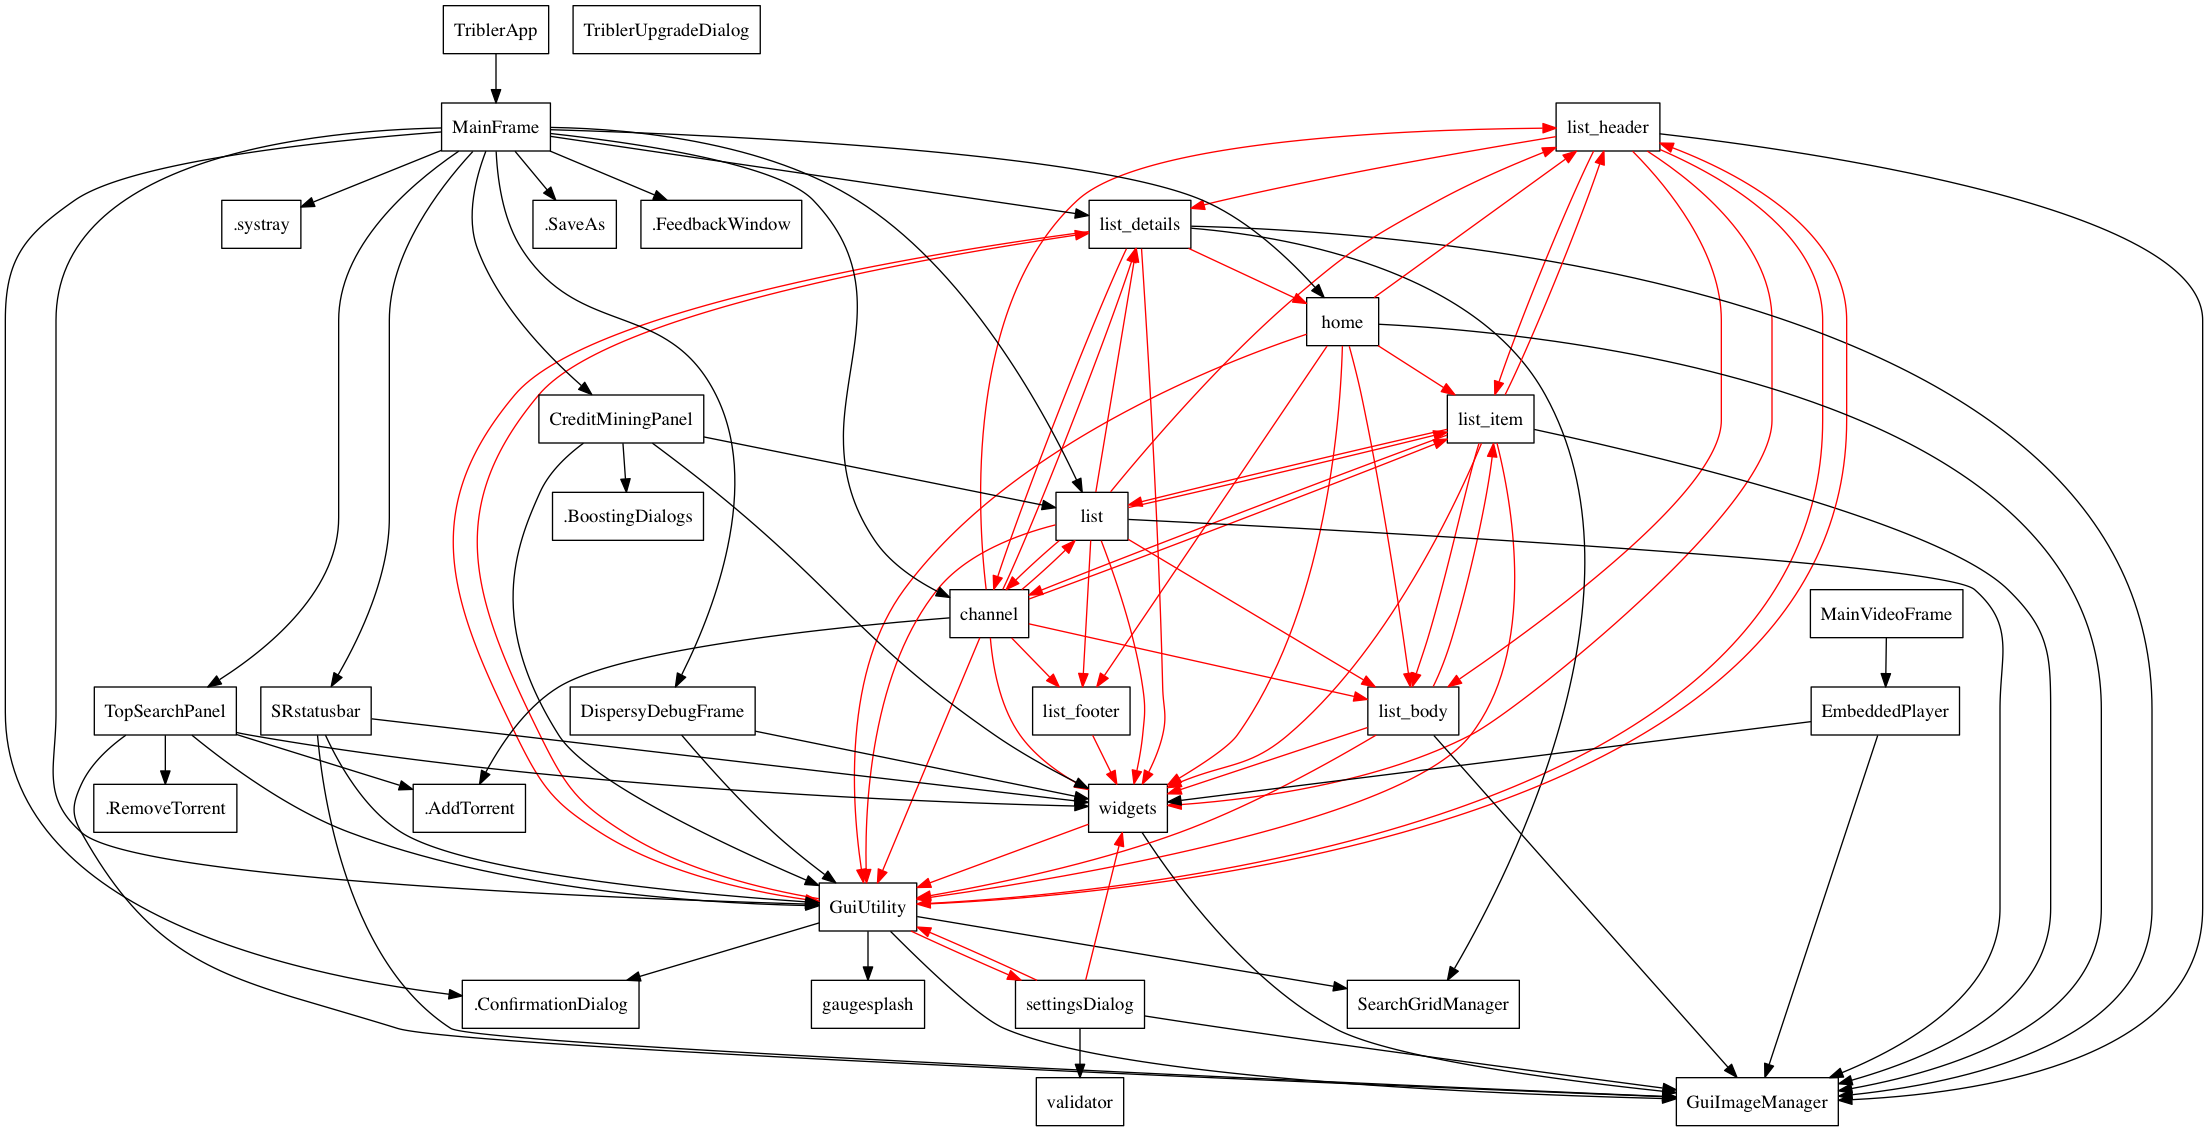
\includegraphics[width=1.0\columnwidth]{images/problem_description/wx_cycles}
	\caption{A generated import graph of the GUI code base. A red edge indicates that this edge is part of an import cycle.}
	\label{fig:wx-import-graph}
\end{figure}

While the current decade of software engineering provides a plethora of visual designers that requires barely any hand-written code, our whole user interface is built using code that's unmaintained and hard to understand. Many features and visual elements in the GUI are unnecessary and unintuitive, contributing to (visible) technical debt. Finally, the user interface has been written with the \emph{wxPython} framework which is unmaintained since late 2014. The library builds upon native APIs, i.e. Cocoa on OS X and Win32 on Windows. While the library claims to be cross-platform with a native look and feel, various features in Tribler are limited to a subset of the supported platforms due to incompatibilities.

\section{Unstable and incomplete testing framework}
Testing is the responsibility of every developer that contributes to Tribler. Over the past ten years, this responsibility has been completely neglected by the majority of contributors, leading to a significant amount of \emph{testing debt}. This is clearly visible in Figure \ref{fig:tests-ratio-tribler} where we plot the ratio between the amount of code lines in the test suite (TLC) and the number of code lines related to production code (PLC). Tribler has a structural lack of well designed (unit) tests. Currently, around 100 tests are present that cover 71,2\% of the source lines of code located in the Tribler core. Many of these tests are taking over half a minute to complete and are depending on a running Tribler session. Only a small fraction of the test suite has characteristics of unit tests. Having tests that are doing a broad range of operations, inevitably leads to undesired side-effect and failing tests. As far as we are aware, no attempt has been made to mock components of the system to simplify testing and to focus on the specific part of the system that has to be verified.\\\\
There is an additional flaw that contributes to the instability of the current test suite. A significant part of the test suite is depends on external network resources, ranging from torrent trackers and seeders to other peers in the decentralized Dispersy network. This fragile architecture gives rise to failing tests due to unavailable nodes, unexpected responses from external peers and other unpredicted circumstances.\\\\
In general, well designed tests exclude any dependency on external resource that is outside the control of the developer. This can be achieved by mocking method calls to return dummy data. Additionally, one can make sure that the external resource is available in the local testing environment. For instance, when a test is dependent on a specific torrent seeder, a local \emph{libtorrent} session can be started that seeds this torrent.\\\\
While Tribler is packaged and distributed on multiple platforms, the tests in our continuous integration environment are only executed on a machine running a Linux operating system. Limiting test execution to one platform, lowers the overall code coverage and covers platform-specific bugs\cite{beller2016oops}. Attention should be given to make our test execution multi-platform.

\begin{figure}[h!]
	\centering
	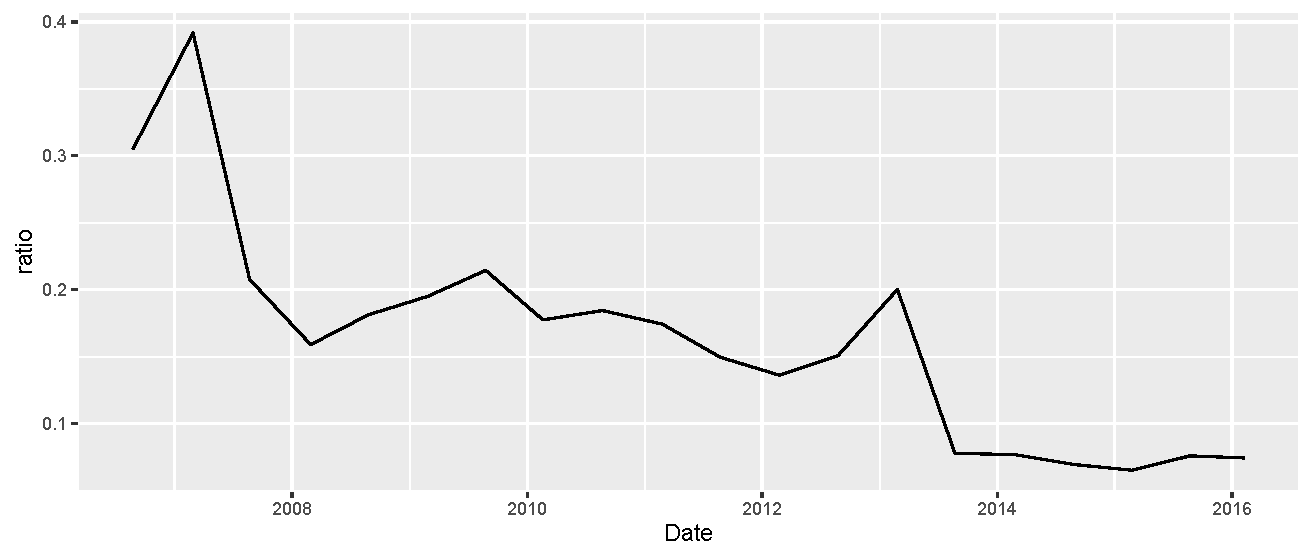
\includegraphics[width=1.0\columnwidth]{images/problem_description/tests_ratio_tribler}
	\caption{The ratio between the lines of code in the tests package and other lines of code over time.}
	\label{fig:tests-ratio-tribler}
\end{figure}

%\section{Quality Assurance}
%The ongoing lack of any quality assurance measure has led to several concerns. In this Section, some of the problems regarding quality assurance will be addressed.
%
%\subsection{Test Suite}
%Tribler has a structural lack of proper designed unit tests. Currently, there are 99 tests and 48.970 lines of code in the Tribler module (excluding code in the Dispersy framework). Many of these tests are taking over half a minute to complete and are bootstrapping an extensive Tribler session. Only a small fraction of the test suite has the characteristics of unit tests. Having tests that are doing a broad range of operations, inevitably leads to undesired side-effect and failing tests. No single attempt has been made to mock components of the system to simplify tests and focus on the part of the system that has to be verified.\\\\
%To illustrate this problematic situation in more detail, the tunnel community is taken as example. The tunnel community allows users of Tribler to anonymously download content and is one of the most anticipated features of the software. The current test suite contains no single unit test that is focussed on this part of the code. Instead, there are several unstable integration-like tests that are starting up a graphical user interface and perform an anonymous download. While one might argue that having such a test might be sufficient for regression testing purposes, this test does not fully cover the source code and any code related to error handling is completely uncovered.\\\\
%There is one more factor that contributes to the instability of the current test suite. A significant part of the test suite is depending on external network resources, ranging from trackers and seeders for a specific torrent to other peers in the decentralized Dispersy network. This fragile architecture gives rise to failing tests due to unavailable nodes, unexpected responses from external peers and other unpredicted circumstances.\\\\
%In general, well designed tests exclude any dependency on external resource that is outside the control of the developer. This can be achieved by mocking method calls to return dummy data. Additionally, one can make sure that the external resource is available in the local testing environment. For instance, when a test is dependent on a specific torrent seeder, a local libtorrent session can be started that seeds this torrent.
%
%\subsection{Testing Environment}
%Tribler uses a Jenkins environment to automate the testing of new Pull Requests (PRs). These tests are only executed on a Linux server. Tribler itself, however, is also packaged and distributed for Windows and OS X. According to the GitHub download statistics, the Windows and OS X distributions account for 91\% of the downloads\footnote{https://api.github.com/repos/tribler/tribler/releases/latest}. Not running any test on this platform is a missed opportunity to identify platform-specific errors. Moreover, any conditional in the source code that is only executed on a specific platform, remains completely uncovered and untested.
%
%\subsection{Documentation}
%The responsibility to maintain a proper and up-to-date documentation base for current and new developers has been completely neglected during the lifespan of the Tribler project. Except for some general information about the project, there is a minimal amount of information available about the system. Since the process of familiarization with the source code is very hard, Tribler has become an unattractive open-source project to contribute to.
%
%\subsection{Outdated Dependencies}
%The Tribler code base has many dependencies on other libraries. At the time of writing, Tribler depends on at least 20 other python libraries. Apart from that, we need libraries for testing and packaging the code. Keeping these libraries up to date, is a necessary and important process.\\\\
%Outdated libraries might lead to compatibility issues and workarounds. For packaging Tribler on Windows, we are using \emph{py2exe}, a library that is not maintained since 2008. Usage of \emph{py2exe} might be dropped in favor of more maintained and mature libraries, for instance, \emph{PyInstaller}.
%
%
%\section{Code quality}
%In the previous Section, the lack of quality assurance and the consequences of this has been elaborated. In this Section, the focus will shift to the code itself. Identified issues in the current structure of the source code will be discussed.
%
%\subsection{Graphical User Interface}
%The current Graphical User Interface (GUI) of Tribler is written with the wxPython library. The GUI accounts for just over 20.000 source lines of code (SLOC), making up 33\% of the Tribler code base which is significant.\\\\
%The code base of the GUI is has been subject to various refactoring cycles. This leads to a very complex and hard to understand package of code. Technical debt is clearly visible in this part of the code base. Moreover, the interface is plagued with many useless and hidden features that are contributing to the complexity of the code. A clean slate approach with a more mature and user-friendly libraries seems to be the solution that could benefit Tribler the most.\\\\
%The current decade of software engineering provides many alternative tools and libraries that allows to build a visually appealing, platform-independent interface with a minimal amount of code. For instance, the popular and mature Qt framework allows developers to specify their layout in a visual designer.
%
%\subsection{High Coupling between modules}
%The user interface and core of Tribler are interleaved to such an extent that it is inconvenient for developers to test out specific features without making changes to the GUI. Providing a minimal Tribler service that only runs the core code and removing the dependencies between the core and user interface will boost the productivity of developers. An interface can be provided to provide necessary  interactions with the core. There are some more occurrences of dependencies between modules which should be removed. For instance, a full Tribler session object is passed to the constructor of the main database class while a path to the destination location of the database file suffices.\\\\
%By separating modules from each other, the ease of maintainability can be improved since developers do not need to worry about errors that are propagating to other module dependencies. Separation also leads to a code base that is easier to understand.
%
%\subsection{Inconsistent Code Style}
%After the contribution of 44 developers, numerous code styles across the code base can be identified. This leads to an inconsistent code base. There is absolutely no appliance to the PEP8 guidelines which is based on the fact that the current source code contains a sheer amount of 1644 violations.

%Refactoring overview 5-pages

%This chapter show a general overview of all the various large and small contributions made to boost the health of the code base. In total over 13000 lines of code have been altered. 33 pull requests accepted.
%GUI screenshots, before, after
%remove DB calls from GUI.
%Github screenshots with altered lines of code.
%progressive JSON API.

%Quality Assurance infrastructure 8-pages

%In the previous chapter a general overview is provided of the numerous changes to the code base. Now we focus on the specific changes for quality assurance in more detail. Key change is 
%splitting of the code base into two parts to make them easier to maintain.  
%-documentation, easier to contribute, improved learning curve, REST API.
%software performance regresssion-graphs
%evolution of code coverage

%Experimental results 10-pages GRAPHS

%We now focus on performance experiments of our new Tribler code base and demonstrate the key improvements.

%Startup time graph, 10 runs + 10 runs new
% + breakdown, checkpoints..
%remote search
%download speed
%memory usage+stress test, while doing lots of REST API calls.
%content discovery speed, Subscribe channels experiment: 1,5,10,15,25 joined channels and resource usage.

%...
\chapter{Architecture and Design}
\label{chapter:architecture}

Before we reach the point of discussing a new future-proof, modern architecture and design of Tribler, the evolution of the Tribler architecture  throughout the last 10 years will be elaborated. Understanding the past decisions regarding architecture and design, will help us to shed light on the question why Tribler has accumulated such an amount of technical debt.\\\\
According to GitHub, Tribler has a total of 44 unique contributors so far. This list is most likely not complete since some work of missing contributors might have been finished by another member of the Tribler team. Searching for \emph{Tribler} in the TU Delft repository, results in a total of 66 hits of which 35 results are contributions in the form of a MSc or BSc thesis.\\\\
The remaining of this chapter will present a historical description of the evolution of Tribler. Next, a new architecture will be proposed and discussed in detail. This will lay the foundations for the next decade of research in the area of peer-to-peer network and anonymity.

\section{Tribler: A social-based peer-to-peer system}
Tribler started out as fork from \emph{Another BitTorrent Client} (ABC), an improved BitTorrent client. ABC is based on \emph{BitTornado} which extended from the \emph{BitTorrent} core system, written by Bram Cohen. In the current code base of Tribler, various references to ABC can be found, mostly notable in the naming of files, variables and classes.\\\\
In 2007, the first major research paper was published, describing Tribler as a social-based peer-to-peer system\cite{pouwelse2008tribler}. The key idea is that social connections between peers in a decentralized network can be exploited to increase usability and performance of the network. This is based on the idea that peers belonging to a social group are not likely to steal (free-ride) bandwidth from each other. The system architecture of the system is visible in Figure \ref{fig:tribler-architecture-2008}. In the remainder of this Section, the most important components of the architecture as described in \cite{pouwelse2008tribler} will be explained in more detail.

\begin{figure}[t]
	\centering
	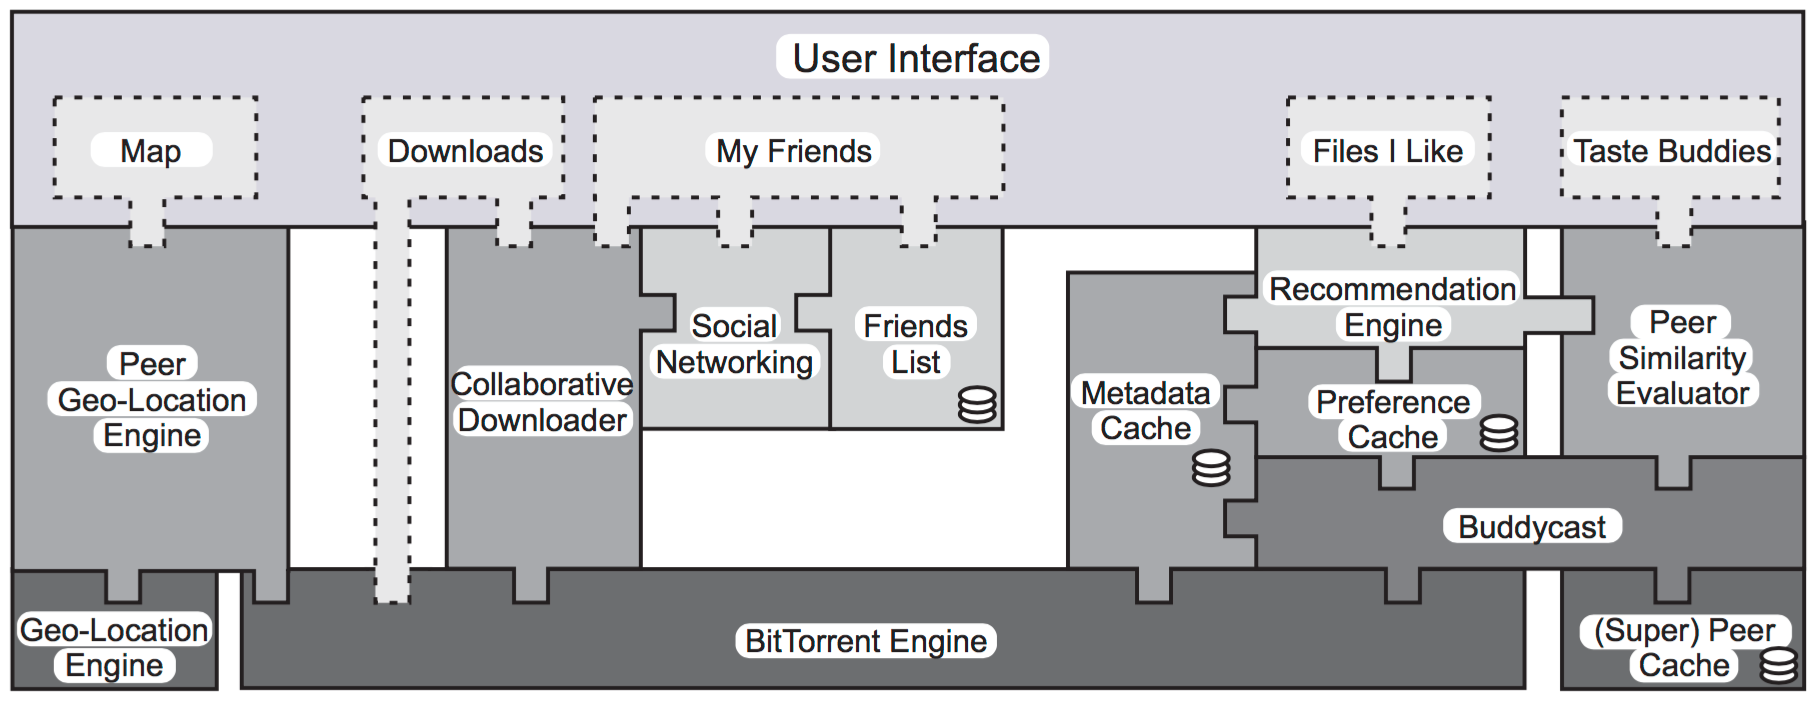
\includegraphics[width=0.9\columnwidth]{images/tribler_architecture_2007}
	\caption{The system architecture as described in \cite{pouwelse2008tribler}.}
	\label{fig:tribler-architecture-2008}
\end{figure}

\subsection{Collaborative Downloads}
The BitTorrent engine allows the mechanism to download and seed torrent files using a BitTorrent-compatible protocol. In addition, the module allows usage of the \emph{collaborative downloader} module which significantly increases download speed by exploiting idle upload capacity of online friends.\\\\
The protocol to facilitate collaborative downloads is called \emph{2Fast} and the idea is that a user invokes the help of friends to increase download speed of his files. The protocol uses social groups where members who trust each other collaborate to improve their download performance. Peers that are participating in a social group are either \emph{collectors} or \emph{helpers}. A collector is a peer that is interested in obtaining a complete copy of a particular file. A helper is a peer that is recruited by a collector to help downloading that file.

\subsection{Peer Geo-Location Engine}
The \emph{Peer Geo-Location Engine} is an engine built on top of a module that enables geographical lookup of IP addresses (\emph{http://hostip.info}). When a peer downloads a file, peers in the download swarm are displayed on a map in the user interface.

\subsection{Content Discovery and Recommendation}
The \emph{BuddyCast} algorithm is designed to make recommendations and to enable peer and content discovery. BuddyCast is an epidemic protocol which works as follows: each peer in the network maintains a number of taste buddies with their preference lists and a numer of random peers without any information about their preferences. Periodically, an \emph{exploration} or \emph{exploitation} step is performed. When an exploration is executed, the peer connects to one of its taste buddies. The peer connects to a random peer if an exploitation step is performed. When the connection is successful, a \emph{BuddyCast} message is exchanged.\\\\
A Buddycast message contains the identities of a number of taste buddies along with their top-10 preference lists, a number of random (and fresh, see below) peers, and the top-50 preferences of the sending peer. The age of each peer is included in the message to help others know the freshness of peers. After the BuddyCast messages are exchanged, the received information is stored in the local database of each peer. To limit redundant messages, each peer maintains a list of recently contacted peers.

\section{Shaping the next generation of internet TV}
In 2008, the European Union funded the P2P-Next research effort\cite{p2pnextpressrelease}. The project was active starting from 2008 to 2012 and planned to conduct a large-scale technical trial of new media applications running on a wide range of consumer devices, using peer-to-peer technologies. Tribler has been the main subject of research during the P2P-Next project by TU Delft. This Section will explain the conducted research and architectural evolution during the P2P-Next project.

\subsection{Tribler 4.0}
The next version of Tribler, version 4.0, got released in 2007\cite{tribler4tf}. Many features from the 3.x release cycles are taken over and some new functionality have been added. Using an embedded video player, users can play videos (while being downloaded) directly from within the user interface. This video player is powered by the VLC library and bindings for the user interface library, \emph{wxPython}. Tribler 4.0 allows users to remotely search for content inside the Tribler network but also content on YouTube and Liveleak. The search results are displayed in a YouTube-like thumbnail grid. The interface of Tribler 4.0 is displayed in Figure \ref{fig:tribler4}.

\begin{figure}[t]
	\centering
	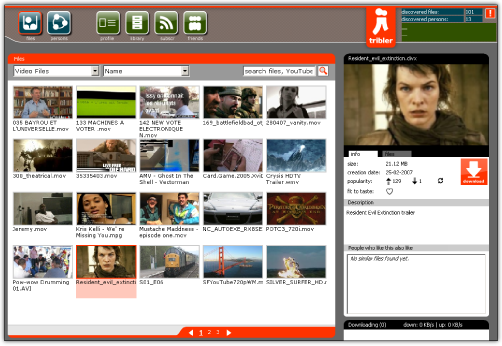
\includegraphics[width=0.8\columnwidth]{images/tribler4}
	\caption{The user interface of Tribler 4.0.}
	\label{fig:tribler4}
\end{figure}

\subsection{Tribler 5.x}
The development of Tribler continued with the release of Tribler 5.0 in 2009\cite{historyoftribler}.  The interface got a complete overhaul, introducing a more dark theme, which was replaced by a white theme a short while after the release. In the 5.x series, several improvements to Tribler itself and the user interface has been made. The focus of Tribler 5.0 has been on remote search and downloads. The thumbnails have been dropped and the search results are displayed in a paginated list instead.\\\\
Tribler 5.1 contained some major improvements to the user interface, thanks to the feedback of the community. A new major addition have been added to Tribler 5.2: the concepts of channels, similar to YouTube, has been introduced. One goal of channels was to prevent spam inside the network by favouring content in more popular channels. The popularity indicator associated with each torrent got removed but has been placed back later. In Tribler 5.3, all custom widgets got replaced by native buttons, creating a more native feel on each platform. A tag cloud has been added to the home page of Tribler to help users determine which content they possibly want to look for. Moreover, the paginated list was replaced by a single, scrollable list of items. Tribler 5.4 introduced a magic search feature where similar search results are collapsed using text similarity functions and digit extraction. This leads to a much cleaner and comprehensive results list when searching.\\\\
The final release in the 5.x series, Tribler 5.9, bought some major additions. The complete BuddyCast core has been rewritten, moving away from a TCP overlay to an implementation based on UDP, bringing huge benefits to the compatibility with NAT-firewalls. Also, \emph{libswift} has been introduced as the new download engine, providing download capabilities over UDP, removing the TCP layer from libtorrent.

\section{Tribler 6.x}
Shortly after the release of Tribler 5.9, Tribler 6.0 is released where a complete new user interface has been implemented. This version contained also some minor bug fixes that increased performance and usability. After the release of 6.0.1, several smaller releases (6.1, 6.2 and 6.3) were released. The focus shifted toward anonymous downloads and end-to-end encryption. These features were part of the Tribler 6.4 release, providing an experimental anonymous download mechanism and hidden seeding services. Moreover, the \emph{libswift} dependency got dropped since it was not stable enough. This release also introduced the TFTP protocol, used to transfer torrent files between peers in Tribler. The next release, Tribler 6.4.1, contained some major security fixes after an external code review.\\\\


\section{Defining the future of Tribler}
In the previous Section, the evolution of Tribler has been evolved, up to the current architecture. We now turn our attention to the future of Tribler and propose a new architecture that will enable Tribler for another 10 year of research. The proposed architecture is visible in Figure \ref{fig:tribler7}. This architecture follows a layered approach with a clear distinction between the visible layers. This Section will discuss the proposed design and highlight decisions that have been made during the development process.

\begin{figure}[h!]
	\centering
	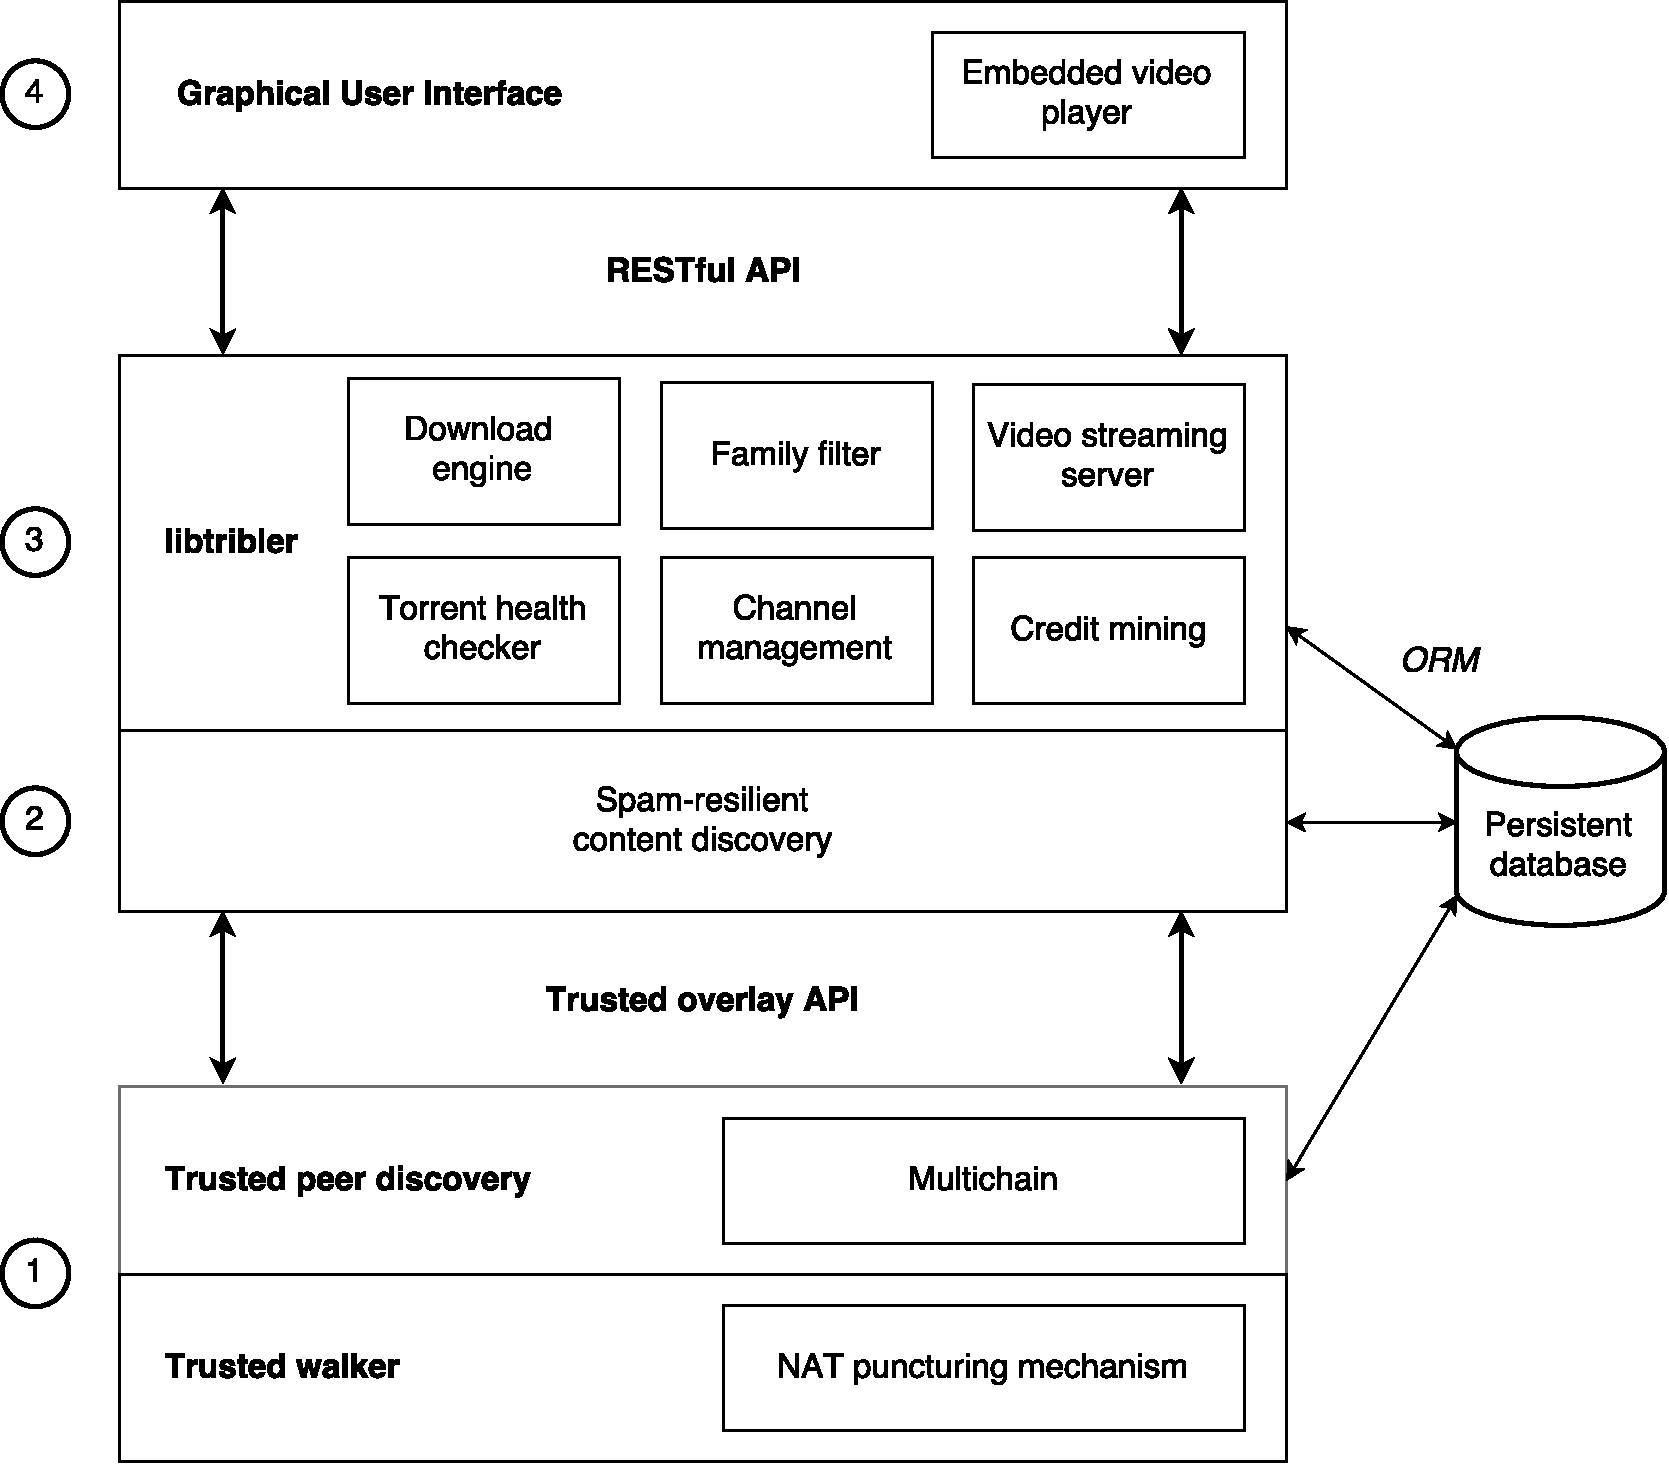
\includegraphics[width=0.7\columnwidth]{images/architecture/tribler7}
	\caption{The proposed architecture of Tribler 7.}
	\label{fig:tribler7}
\end{figure}

\subsection{Trusted Peer Discovery}
The trusted walker is located at the lowest layer of the architecture and is the central component for discovering other peers. At the moment, Dispersy is responsible for discovering other peers in the Tribler network. This mechanism will be replaced by a trusted walker that is used by the Multichain\todo{beter uitleggen}.

\subsection{Libtorrent and Content Discovery}
Above the walker primitives explained in the previous Section, we find two components that are already present in the current system. The popular \emph{libtorrent} library is used to facilitate downloads. Libtorrent is written in C++, however interfaces for other programming languages such as Python, Go and Java are available. Libtorrent uses an alert mechanism to notify the program that is using the library about events in the library, such as download state transitions, peer discovery or completion of a metainfo lookup. The current way of using \emph{libtorrent} in Tribler requires minimal changes in the proposed design, except for some minor refactoring and cleanup of the current code.\\\\
The content discovery components allows users to discover and search for available torrents, channels and playlists in Tribler\todo{afmaken}.

\subsection{libtribler}
Test

% http://delivery.acm.org/10.1145/2080000/2072433/p739-zeilemaker.pdf?ip=145.94.5.138&id=2072433&acc=ACTIVE%20SERVICE&key=0C390721DC3021FF%2E512956D6C5F075DE%2E4D4702B0C3E38B35%2E4D4702B0C3E38B35&CFID=816981133&CFTOKEN=23604061&__acm__=1469268778_0dc54a276c6ce7abce65547df9722e66

% TODO explain threading model
\chapter{Paying Off the Debt}
\label{chapter:refactoring}
In Chapter \ref{chapter:problem-description}, the extraordinary amounts of technical debt that Tribler has accumulated over the past decade has been highlighted. We presented the architectural evolution from a historical perspective and proposed a new robust and future-proof architecture in Chapter \ref{chapter:architecture}. The top-level components of this new architecture, the GUI and RESTful API to communicate between the user interface and libtribler, have been implemented and discussed in Chapter \ref{chapter:towards-new-architecture}. We did not focus yet on libtribler, which can be considered as the core of the Tribler platform. Shaping libtribler to fit in the proposed architecture of Figure \ref{fig:tribler7}, requires some invasive refactoring efforts. Since this might be the most important component in our system, we will investigate libtribler in more detail and determine how we can identify and pay off the accumulated technical debt in the core. A summary of the re-engineering efforts conducted during this thesis work is displayed in Table \ref{table:refactoring-summary}.\\

\begin{table}[h!]
	\centering
	\begin{tabular}{|l|l|}
		\hline
		\textbf{Lines modified} & 765 \\ \hline
		\textbf{Lines added} & 12.429 \\ \hline
		\textbf{Lines deleted (without old GUI)} & 12.581 \\ \hline
		\textbf{Lines deleted (with old GUI)} & 25.010 \\ \hline
	\end{tabular}
	\caption{A summary of refactoring efforts as conducted during this thesis work, excluding the work on the new GUI.}
	\label{table:refactoring-summary}
\end{table}

Roughly, we can identify five different types of technical debt\cite{seaman2011measuring}: \emph{code debt}, \emph{testing debt}, \emph{infrastructure debt}, \emph{architectural debt} and \emph{documentation debt}. Tribler shows symptoms for every of the summarized types of technical debt.\\\\
We argue that refactoring in a dynamic typed programming language like Python is harder than when using a statically type language: information about errors when renaming is not observed before runtime because of the lack of type information. This issue becomes apparent when trying to rename a variable using a Python Integrated Development Environment (IDE): the application logic might miss various occurrences when performing the renaming operation and we only become aware of this issue when either running Tribler itself or when executing the test suite. This shows the importance of having a solid, extensive test suite before we start to refactor major components in the system and we started with creating improvements to create a solid foundation for our refactoring efforts. Improving the test suite first has an additional advantage: by studying the test code, we can familiarize ourselves with the code base. Also, a review of the test code may help to us to understand the structure and detect code smells in the production code\cite{van2002video}.\\\\

%\section{Software Ageing}
%We start the discussing with introducing and discussing the term \emph{software ageing}, which we think is a phenomena that is particular visible in Tribler and that helps us to find root causes of the introduction of technical debt. Software ageing is a problem in a society that is dependent on all kinds of software. The term has been coined by Dave Parnas in his talk about software ageing in 1994\cite{parnas1994software}. He points out two major reasons why software ageing is a problem. The first is the lack of movement when software fails to meet the requirements of an always-changing environment: software that users perceived as state-of-the-art several decades ago, might now be considered as legacy software, mainly due to performance reasons. For instance, where a latency of several seconds when performing a remote search in Tribler might have been acceptable several years ago, users now expect system that responds to queries within a second.\\\\
%The second reason is in particular interesting since we think this is one of the most important reasons why Tribler has evolved to the complex, hard-to-understand architecture it is today and Parnas references to this phenomena as \emph{ignorant surgery}. Changes made by people who do not understand the original design concept almost always cause the structure of the program to degrade. This is especially true for the development process of Tribler which had many contributors who are making changes to specific parts of the architecture, often ignorant about the design concepts of the original authors of the code. Moreover, some developers might not be satisfied with the implemented design and decide to change the architecture to suit their own needs, possibly leading to an even more complex system.\\\\
%There are several approaches on how we can prevent or limit the process of software ageing. The first step towards the right direction, is to think about a design that is subject to change by applying the old slogan "design for change". This slogan is reflected in the flexibility requirement of the proposed architecture in Chapter \ref{chapter:architecture}. Various design principles are helpful to prepare a system for changes such as separation of concerns and using abstractions, however, many programmers fail to correctly apply these changes in software, either due to ignorance or recklessness. We should also note that it is notoriously hard to consider and think about possible changes in the future before starting to write code. This is in particular applicable to Tribler, where often a short-term research goal should be achieved: developers are writing a piece of software that they need for obtaining experimental results. New features are often the product of a publication or research project which are most likely not scheduled when designing an architecture of Tribler. In fact, it is not even certain that new features will be added after a specific release, since Tribler is not considered a complete commercial product that should meet customer's expectations (although we should try to achieve the highest level of user satisfaction).\\\\
%Design decisions taken during the development process are often not  documented. Developers fail to see the need for a proper documentation base and are proposing that the code is the documentation itself. However, this only works if you are following the structure they are using. Sometimes, it is more successful to communicate ideas on a higher-level, natural language that allows for less disambiguation. Tribler used to keep track of several design documents that describe the architecture, user interface decisions and research results, however, these documents are outdated and at the moment, there is no clear up-to-date description of the architecture. The lack of software artifacts will be discussed in more detail in Section \ref{sec:software-artifacts}.\\\\
%Parnas considers another option to limit software ageing: code reviews. For years, Tribler developers have created many new features which are not peer-reviewed by anyone, leading to a mix of different programming styles. Code reviews are an essential part in the software development process and should not be neglected.\\\\
%While prevention is a good medicine, we should define method that describe how we should deal with aged software. First of all, we can apply the methods we describe: change for design, code reviews and the construction of a proper documentation base. Modularisation of a system can be used to quicker identify components that are changing over time. When a product gets out of control, we should do a major restructuring of the product.

%\section{Influences of Python on software metrics}
%Tribler is written in: Python, an accessible, easy-to-learn language that is widely used in scientific applications. It is a high-level language, allowing one to express constructs with only a few lines of code. One of the most distinguishable properties of the language is that it is dynamically typed, which means that the type of a variable is not known at compile-time. This is in contrast to static typing, where this type is known to the compiler. The dynamic nature of the language has consequences on the way programmers are writing their code. A dangerous pitfall is that developers are making wrong assumptions about types of variables, leading to bugs that are only visible on runtime. Even then, it is not guaranteed that these kind of errors reveal themselves since they might be located inside a branch that is entered in a small amount of the application executions. Advantages of dynamic typing are apparent in testability since it is easier to mock objects during test execution.\\\\
%Dynamic typing also influences generated software metrics. While import graphs might give a good indicator of dependencies, they do not tell the whole story. In fact, there might be dependencies that are not visible in a generated import graph. These 'hidden' dependencies are often made between classes using the \emph{dependency injection} (DI) design pattern, a technique to not denote dependencies in the source code. For instance, if a class \emph{A} needs a particular service, this service is passed as parameter in a method call to \emph{A}. Dynamic typing makes it harder to capture such dependencies since almost no any information about types of attributes within a class can be determined at compile-time. The DI design pattern is very commonly used in Tribler and it is the preferred way to let components know about other components.

\section{Investigating the Debt}
It is hard to get accurate numbers on the amount of technical debt since it is not always clear what we consider as technical debt. When a decision to pay off (a part of) the debt is made, developers might run into unexpected situations that take longer than expected, especially if working with unfamiliar code written by other developers. This makes estimations of the amount of work required unreliable. Several tools exist to monitor and estimate technical debt, the most prominent being CAST\footnote{http://www.castsoftware.com} (commercial) and SonarQube\footnote{https://sonarqube.com}\cite{falessi2015towards} (open source). In this section, we will use SonarQube to track and identify the amount of technical debt in Tribler by setting up a SonarQube server to identify technical debt, bugs and vulnerabilities in the Tribler project. We do this for the old and new user interface and for the Tribler core, before and after our refactoring efforts. The reported results are summarized in Table \ref{table:sonarqube-metrics-summary}. We should emphasize that a small amount code smells are very hard, if not impossible to fix in our application.\\

\begin{table}[h!]
	\centering
	\begin{tabular}{ l | l | l | l | l |}
		\cline{2-5} & \textbf{SLOC} & \textbf{Code smells} & \textbf{Bugs} & \textbf{Estimated debt}\\ \hline
		\multicolumn{1}{ |l| }{wxPython GUI} & 20.080 & 2.139 & 11 & $\pm$ 21 days\\ \hline
		\multicolumn{1}{ |l| }{Qt GUI} & 2463 & 14 & 0 & $\pm$ 1 hour\\ \hline
		\multicolumn{1}{ |l| }{Tribler core (before refactor)} & 15.732 & 365 & 6 & $\pm$ 4 days\\ \hline
		\multicolumn{1}{ |l| }{Tribler core (after refactor)} & 15.700 & 117 & 0 & $\pm$ 2 days\\ \hline
	\end{tabular}
	\caption{Software metrics as reported by SonarQube.}
	\label{table:sonarqube-metrics-summary}
\end{table}

The most interesting observation is that the wxPython GUI contains around five times more technical debt than the Tribler core and contains almost six times more code smells. To better investigate which files suffer from the most technical debt, SonarQube provides a bubble chart where the relation between the amount of technical debt, the number of code smells and the amount of SLOC is visualized. For the wxPython GUI, this bubble chart is visible in Figure \ref{fig:technical-debt-wx-gui}. In this chart, the size of the bubble is correlated to the amount of code smells. The files suffering the most under technical debt are annotated with the file name. By taking Figure \ref{fig:wx-import-graph} as reference, we notice here that the files that contain a high amount of technical debt, are also the files with the most dependencies.\\

\begin{figure}[h!]
	\centering
	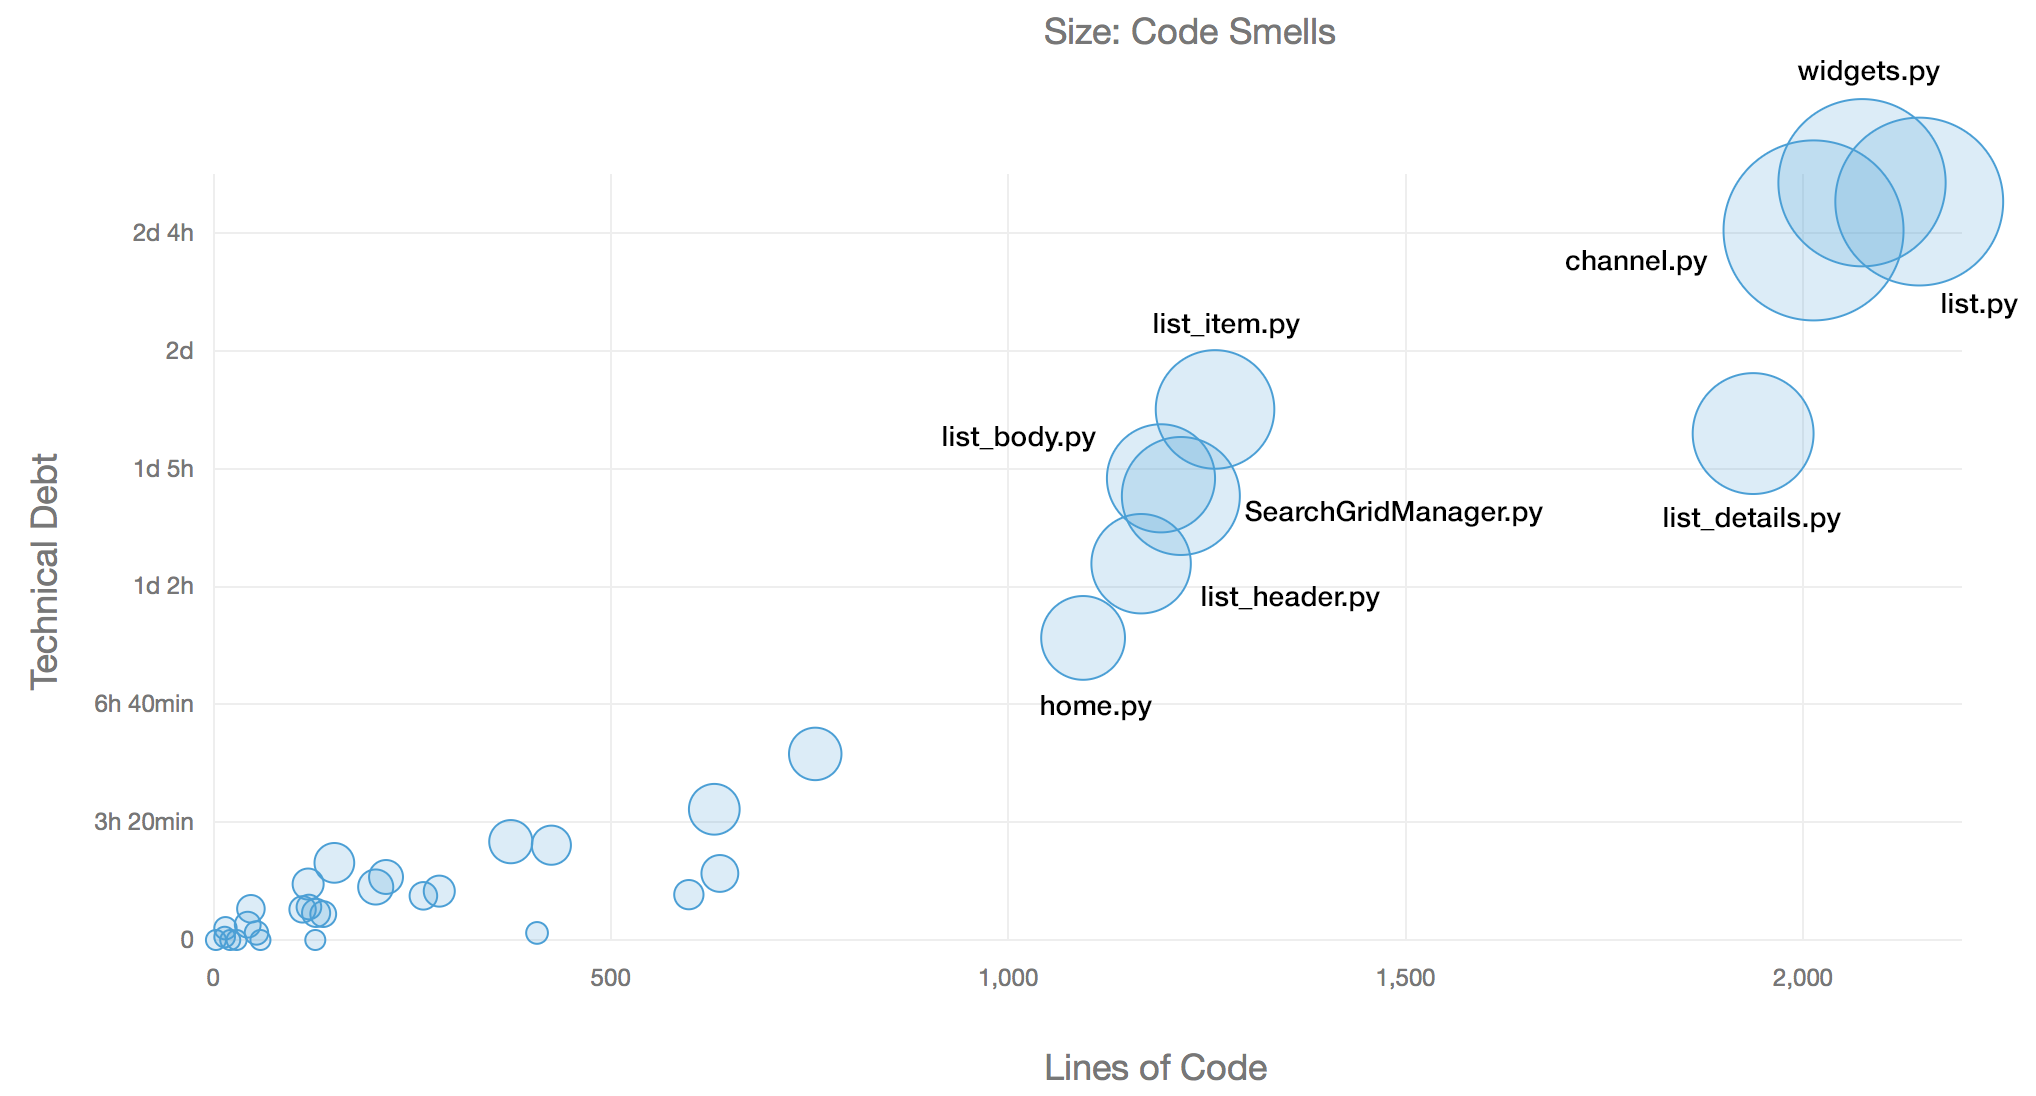
\includegraphics[width=1.0\columnwidth]{images/improving_qa/technical_debt_wx_gui}
	\caption{The amount of technical debt in the wxPython GUI as reported by SonarQube.}
	\label{fig:technical-debt-wx-gui}
\end{figure}

\section{Code Debt}
We now focus on the core of Tribler and present the bubble chart associated with the core package in Figure \ref{fig:technical-debt-core-before}. It is immediately evident that the \emph{SQLiteCacheDBHandler.py} file urgently needs refactoring. This file contains various utility classes to perform common database operation such as retrieval of specific channels, torrents and playlists. This file hosts the implementation of seven classes and our first effort consists of splitting this file into smaller, manageable files where each file contains only one class definition.\\\\
However, we still identify many other files where technical debt is present in the form of code smells. We performed efforts to pay of this debt in the code base and will now summarize the most common identified code smells in the Tribler core package:
\begin{itemize}
	\item The cyclomatic complexity of various methods is too high, indicating that the procedure contains many independent linear execution paths. The cyclomatic complexity as developed by McCabe in 1976\cite{mccabe1976complexity} is a quantitative measure of the number of linear independent paths through a program's source code. This negatively impacts the testability of this method since more distinct tests are necessary to guarantee an adequate coverage of the method. During this thesis, we reduced the complexity of several methods by splitting them.
	\item We identified various methods that could be static. Static methods are meant to be relevant to all the instances of a class rather than to any specific instance. The usage of static methods is beneficial for performance and readability. SonarQube recommends to use static methods where possible and we changed as much recommended methods by SonarQube to static ones as possible.
	\item Naming conventions were not following during the development process and this is most notable in the inconsistency between usage of \emph{CamelCase} practice and the usage of underscore notation. Since we wish to conform to the PEP8 styling guidelines\footnote{https://www.python.org/dev/peps/pep-0008/}, we should use the latter form. Part of our efforts to pay off the identified code debt in the core includes work to rename methods, attributes and variable names to conform to the underscore notation. We should emphasize that some used libraries such as wxPython and PyQt are using the camelCase notation, leading to forced violation of this convention when overriding methods from this library.
\end{itemize}
The bubble chart of the technical debt identified in the core after refactoring efforts described above is visible in Figure \ref{fig:technical-debt-core-after}. We emphasize the difference in scale on the vertical axis here compared to Figure \ref{fig:technical-debt-core-before}. The variance of the code debt has decreased significantly. Notice that the database handler definition files (that were originally located in the larger \emph{SQLiteCacheDBHandler.py} file) still suffers from some technical debt. However, there are many methods in these files that are unused when the new user interface will be deployed and these could be removed at that point. Table \ref{table:sonarqube-metrics-summary} shows the statistics after our refactoring efforts. While we did not solve all code smells, we solve the most prominent occurrences of code debt and contributed to a more useful, maintainable and consistent code base.

\begin{figure}[h!]
	\centering
	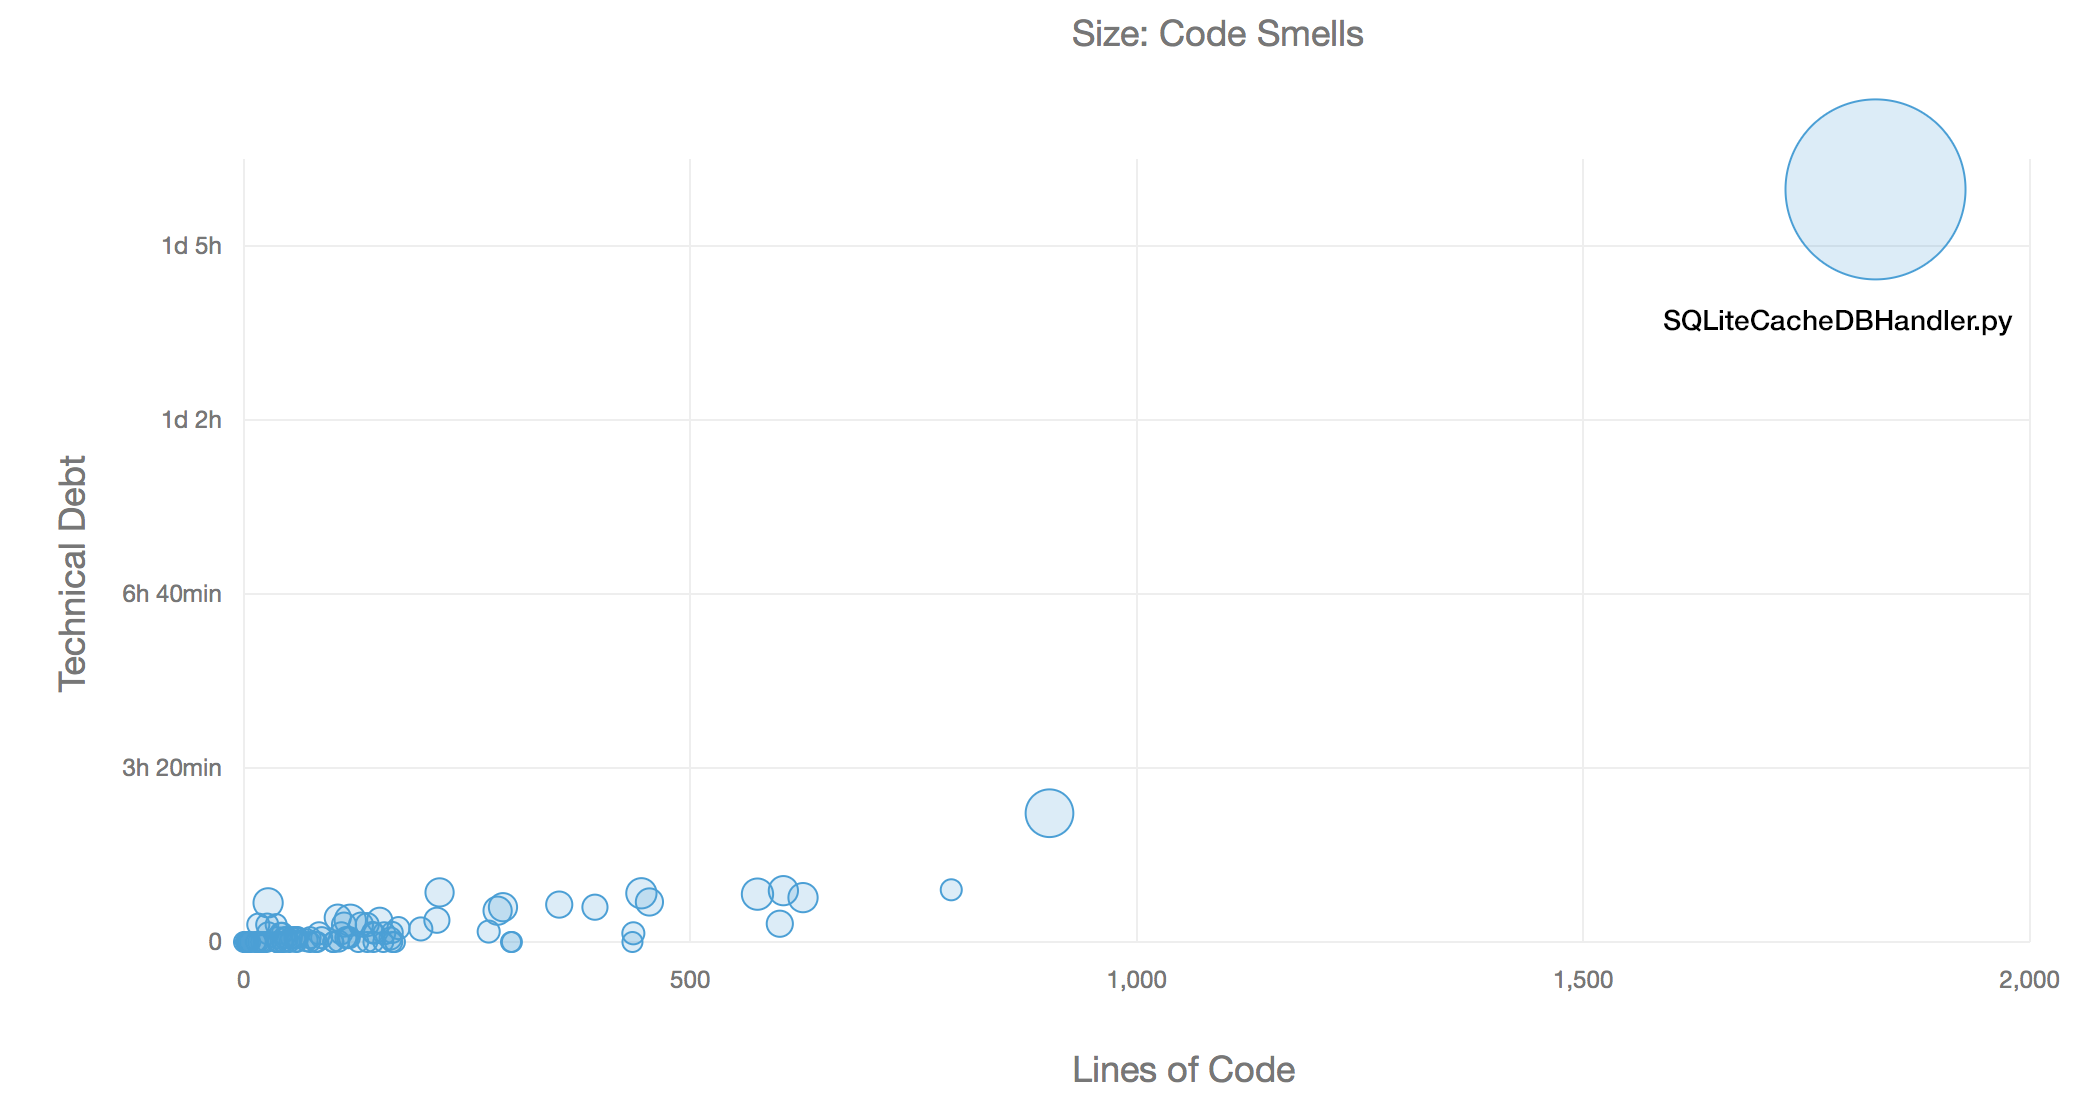
\includegraphics[width=1.0\columnwidth]{images/improving_qa/technical_debt_core_before}
	\caption{The amount of technical debt in the Tribler core package as reported by SonarQube before refactoring.}
	\label{fig:technical-debt-core-before}
\end{figure}

\begin{figure}[h!]
	\centering
	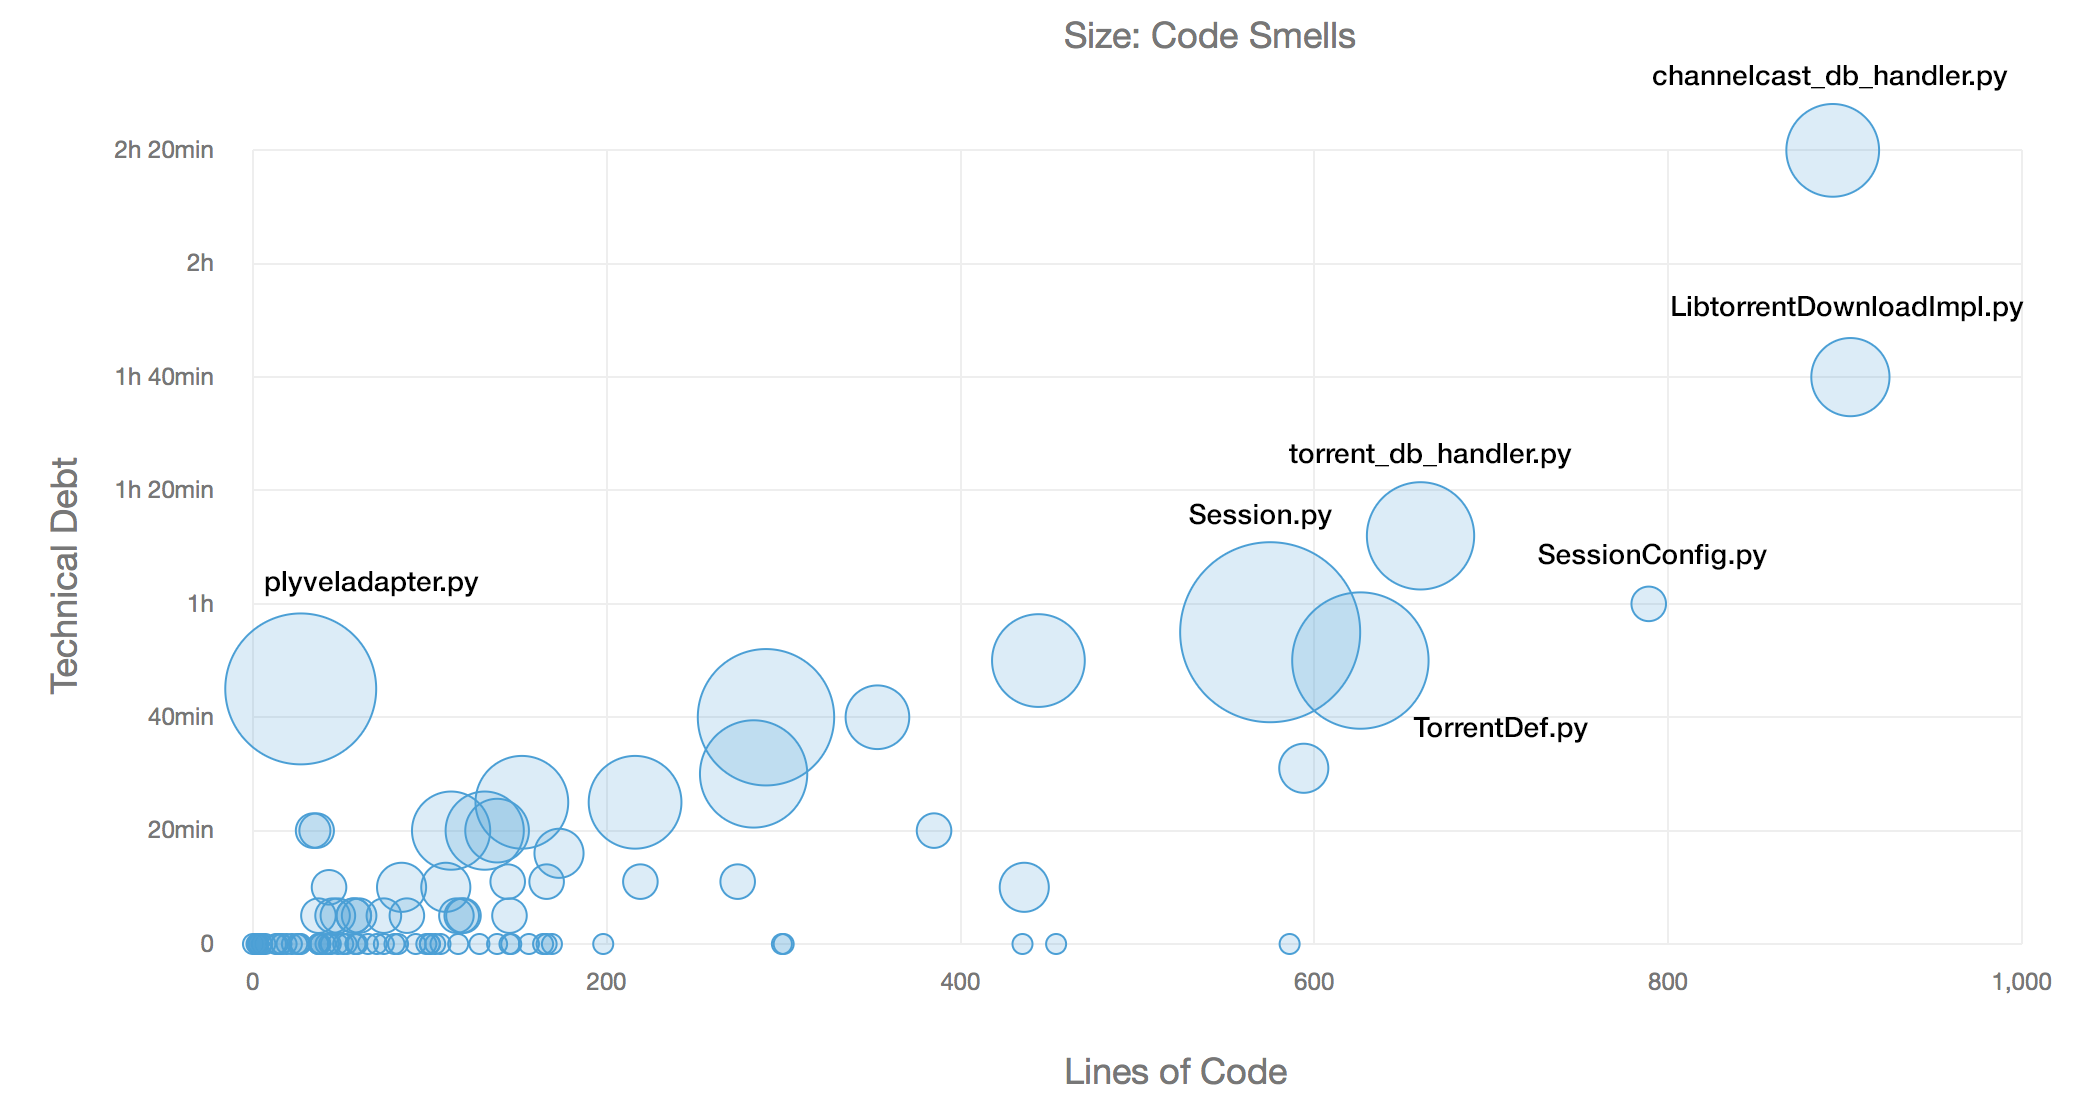
\includegraphics[width=1.0\columnwidth]{images/improving_qa/technical_debt_core_after}
	\caption{The amount of technical debt in the Tribler core package as reported by SonarQube after refactoring.}
	\label{fig:technical-debt-core-after}
\end{figure}

\section{Testing Debt}
The most fundamental way to verify a correct functioning of software is by having an well-designed and stable test suite. A solid test suite leads a to high quality bar, thus introducing a mechanism to keep the amount of technical debt under control\cite{sumit2016unittests}. As pointed out in Chapter \ref{chapter:problem-description}, the current test suite is plagued with unstable and non-functional tests. We will now focus on the performed work to strengthen and stabilize the test suite. A summary of the improvement of various metrics related to the test suite during this thesis is presented in Table \ref{table:test-suite-improvements}. Notice that the number of unit tests has dramatically increased, while the average execution time of a test and the total duration of the tests has decreased.

\begin{table}[h!]
	\centering
	\begin{tabular}{ l | l | l | }
		\cline{2-3} & \textbf{November '15} & \textbf{July '16}\\ \hline
		\multicolumn{1}{ |l| }{Number of unit tests} & 80 & 676\\ \hline
		\multicolumn{1}{ |l| }{Number of assertions} & 117 & 1205\\ \hline
		\multicolumn{1}{ |l| }{Number of failed runs after 10 runs} & 2 & 0 \\ \hline
		\multicolumn{1}{ |l| }{TLOC/PLOC ratio} & 0.06 & 0.14 \\ \hline
		\multicolumn{1}{ |l| }{Total Linux test duration on Jenkins (sec)} & 448 (7 min. 28 sec.) & 350 (5 min. 50 sec.) \\ \hline
		\multicolumn{1}{ |l| }{Average execution time per test (sec)} & 18.90 & 0.85 \\ \hline
	\end{tabular}
	\caption{A summary of improvements made to the test suite between November '15 and July '16.}
	\label{table:test-suite-improvements}
\end{table}

\subsection{Identifying Code Smells in the Tests}
As described in the work of van Deursen et al\cite{van2001refactoring}, there is a difference between refactoring test and production code in a sense that test code often has a characteristic set of code smells, originating from the way tests are structured. Before we start to make major modifications to the test suite, we present a list of code smells identified after a manual code review of the test suite of Tribler. This list is presented in Table \ref{table:tests-code-smells} where each code smell is described and a solution is proposed.\\

\begin{table}
	\begin{tabularx}{\textwidth}{|X|X|X|}
		\hline
		\textbf{Code smell} & \textbf{Description} & \textbf{Solution}\\ \hline
		Dependencies on external resources & Several tests are using external resources outside the test suite, leading to unpredictable and unstable tests. & Remove the dependency on the resource or make sure that the resource is locally available (see Section \ref{subsec:external-network-resources}). \\ \hline
		State leak & The state of a previous executed test is leaking to the next test, mostly notable due to delayed calls left in Twisted after completion of a test. & Make sure that any delayed call in Twisted is correctly removed when the test is finished. \\ \hline
		Too much responsibility & Many tests have multiple responsibilities, testing both parts of the user interface and core components in Tribler. & Make sure that each test is only verifying one small unit in the system. Also implement a separate bundle of tests for the user interface.\\ \hline
		High execution time & There are some tests that are taking long to complete (sometimes over 30 seconds), negatively impacting productivity. This is an indication that the specific test is doing too much. & Identify why the test takes long to complete and shorten the runtime i.e. by breaking the larger test into smaller parts. \\ \hline
		Unclear assertions & Tests that consists of multiple assertion statements often do not annotate this assertion well with a clear and meaningful description when it fails. & Add an annotation with the cause of the failure if an assertion fails so developers can determine the problem quicker.\\ \hline
		Dependencies on a Tribler session & Some tests are starting a full Tribler session while only a small subset of the system is tested, leading to unpredictable circumstances. & Use mocking techniques to inject a mocked session or refactor the component so no session is required to test it. \\ \hline
		Resource writing to source code directories & Various tests are writing resources to source code directories. They might accidentally end up in the Version Control System (VCS) if developers are not noticing these files. & Temporary resources produced by tests should always be written to a temporary directory that is cleaned up after test execution. \\ \hline
		Uncontrolled allocation of local network ports & Some tests that are running in parallel are claiming the same local network port, leading to test failures. & Reserve port ranges to individual parallel test runs or try to avoid the allocation of local ports. \\ \hline
		Timing issues & Some tests are checking for a condition after a fixed time interval. This interval is often based on intuition rather than empirical data. This is particularly dangerous when the test is dependent on external resources. & Refactor the test so the condition check is no longer necessary.\\ \hline
		No usage of code comments & There are no code comments that are explaining the purpose and expected output of the test. & Tests should be annotated with comments to explain the purpose of the test together with the expected in- and output. \\ \hline
		No directory structure in the tests package & There is no directory structure and a large amount of the tests are located inside the same directory. & Restructure the tests package and organise tests in different, logical named directories.\\ \hline
	\end{tabularx}
	\caption{Identified code smells in the test suite of Tribler as of November '15.}
	\label{table:tests-code-smells}
\end{table}

Table \ref{table:tests-code-smells} has been used as reference during the refactoring efforts of the test suite. We fixed most of the outlined code smells. Dependencies on external resources have been reduced to a minimum as explained in Section \ref{subsec:external-network-resources}. The efforts on increasing the stability of the tests is outlined in Section \ref{subsec:instability-tests}. During the refactoring process of tests, we placed clear assertions, added comments in the tests and got rid of managing Tribler sessions as much as possible.

\subsection{Improving Code Coverage}
Code coverage is defined as the percentage of SLOC that is covered by at least one test. Our CI environment offers tools to track the code coverage over time. After each test suite execution, a comprehensive report with detailed information about the coverage is generated. The reported metrics by this report are not accurate enough since some third-party libraries are included in the report, such as the VLC bindings and pymdht, a library to fetch peers from the DHT. We are not responsible for the code coverage of these libraries so we modified the report generation to exclude these files.\\\\
A summary of improvements of the code coverage metric during the span of this thesis are displayed in Table \ref{table:code-coverage-table} where the line and branch coverage is visible before and after this thesis work. Branch coverage is a metric that specifies how well conditional statements are covered and this metric includes the fact that a conditional is either resolved to true or false, possibly influencing the program execution path. In the ideal scenario, we wish to have a set of tests that cover all conditional statements in the case they resolve to true and in the case they resolve to false, thus covering all possible execution paths in the program. This objective gets significantly harder to achieve when dealing with code containing many nested conditional statements. Any conditional statement written has a negative effect on the cyclomatic complexity of a method. The branch coverage is usually lower than the SLOC since it is either hard to cover specific branches or the missing branch might be considered as not unimportant. For instance, this might happen when we have a branch that only logs an event when an error occurs.\\\\
While at first sight it may look like the code coverage has not increased significantly, we should emphasize that the complete architecture of the tests have been overhauled in parallel. Refactoring of the test suite has consequences on the code coverage in other locations in the code base. To elaborate this, the smaller unit tests are not starting the old user interface anymore, leading to a lower coverage in GUI code\\\\
Improving the coverage has been realised by writing small unit tests where we use mocked objects to control the system we are testing. The increase in the amount of unit tests is displayed in Figure \ref{fig:amount-of-tests-increase} where we annotated November '15, when this thesis started. Using mocking is necessary since some components have many other dependencies that are hard to keep under control. Writing tests makes a developer more aware of the written code and it can be considered as a possibility to get familiar with an unknown code base. An additional advantage is that various bugs have been identified and solved during the process of writing additional tests.\\

\begin{table}
	\begin{tabular}{ l | l | l | l | l | }
		\cline{2-5}
		& \multicolumn{2}{ | c | }{\textbf{November '15}} &
		\multicolumn{2}{ | c | }{\textbf{July '16} }\\
		\cline{2-5}
		& \emph{Line coverage} & \emph{Branch coverage} & \emph{Line coverage} & \emph{Branch coverage}\\ \hline
		\multicolumn{1}{|l|}{Tribler core} & 71,2\% & 58,1\% & 81,2\% & 67,3\%\\ \hline
		\multicolumn{1}{|l|}{REST API} & - & - & 99,4\% & 92,7\%\\ \hline
		\multicolumn{1}{|l|}{wxPython GUI} & 65,8\% & 42,7\% & - & -\\ \hline
		\multicolumn{1}{|l|}{Qt GUI} & - & - & 73,4\% & 50,4\%\\ \hline
	\end{tabular}
	\caption{The improvements in code coverage between November '15 and July '16.}
	\label{table:code-coverage-table}
\end{table}

\begin{figure}[h!]
	\centering
	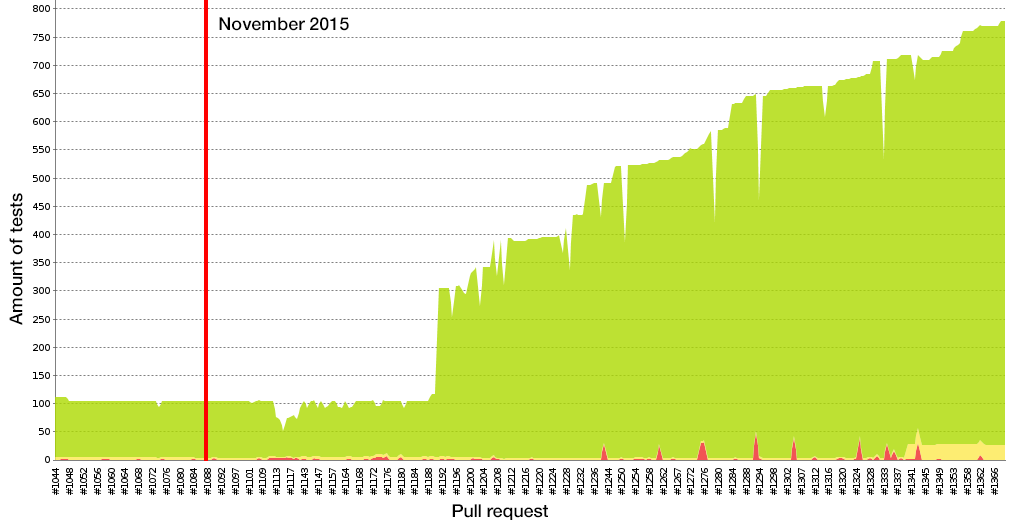
\includegraphics[width=1\columnwidth]{images/improving_qa/test_trend}
	\caption{The number of tests over time until July 2016 (November 2015 is annotated).}
	\label{fig:amount-of-tests-increase}
\end{figure}

In Chapter \ref{chapter:problem-description}, Figure \ref{fig:tests-ratio-tribler} we visualised the ratio between the number of code lines in the tests package and the amount of other code lines. Together with the code coverage, this number can be a useful metric to developers. While one might argue that a high code coverage in conjunction with a low TLOC/PLOC ratio is a desired result, it indicates that the tests are not granular enough and are possibly performing many different operations. A low code coverage with a high TLOC/PLOC ratio indicates that there are some flaws in the tests, possibly that they are testing the wrong components of the system. When starting this work, the code coverage is reasonable but the TLOC/PLOC ratio is very low, indicating that most likely, the tests are not granular enough. This is in accordance with the discovered code smell that individual tests have too many responsibilities.\\\\
After writing additional unit tests, removal of the old user interface and addition of the new one, the new TLOC/PLOC ratio is \emph{0.16} which means that there is roughly one line of test code for six lines of production source code in Tribler. Defining a good TLOC/PLOC ratio is dependent on the used programming language, development methodology and application structure. Discussion on the wiki of Ward Cunningham\cite{c2tlcratio} proposes an optional TLOC/PLOC ratio of 1:1, however, several other ratios have been proposed on the same page such as 2:1 and 5:1. In the work of van Deursen et al.\cite{van2001refactoring}, a ratio of 1:1 is proposed for extreme programming practices. Overall, the trend appears to be that the amount of test line code is around the same or a bit higher than the lines of production code. An important question is whether this proposed ratio is suitable for Tribler. Tribler differs from a commercial software engineering project in the sense that it is used primarily for the purpose of scientific research. When performing research, testing is considered a subordinate task and the main focus is gathering experimental results. The difficulty here is that Tribler is distributed to and used by over a million of users, requiring at least some form of quality assurance. We think an adequate TLOC/PLOC ratio for the Tribler project is between 1:2 and 1:4. With this ratio, we do not spent too much on writing tests while still maintaining a solid test base.\\\\
To make sure that the responsibility of code coverage is not neglected in future work on Tribler, an additional check for each pull request on GitHub has been added that verifies that the code contributed in the respective pull request is covered by at least one test. While this mechanism is not implemented by the author of this thesis, it is an effective way to keep the code coverage metric under control and to make developers more aware of their testing responsibilities.

\subsection{Testing the GUI}
One of the issues identified in the tests package, is the lack of separation between tests that are testing the GUI and tests that are asserting core functionalities of Tribler. This is the main reason that has led to big, individual tests in the old test suite. Since testing is an important aspect of this thesis work, constructing a solid test suite for the user interface has been a prioritized task earlier in the development process.\\\\
User interface testing is a field of software engineering and is part of the application testing methodology. GUI testing can be more involving than unit testing since a user interface might have many different operations and verification of the correct output of an action is often a non-trivial task. A common way of testing user interfaces is a Finite State Machine-based modelling where the user interface is modelled as a state machine that transitions when actions in the user interface are performed\cite{clarke1998automated}\cite{belli2001finite}. Another model to create a test script based on genetic algorithms has been proposed by the work of Kasik et al\cite{kasik1996toward}. While these models might lead to good results when dealing with a large application, consisting of many pages and transitions, we think they are unnecessary to utilize when testing the Qt user interface at this point. Future Tribler research can lead to the implementation of an extensive test suite for the new user interface.\\\\
The test suite of the new Qt user interface utilizes the \emph{QTest} framework. This framework provides various tools to perform non-blocking waits in the tests and to simulate mouse clicks and keyboard actions. An example of a test written with the \emph{QTest} framework is presented in Listing \ref{lst:qtest-sample}. This test has the following execution flow: after the interface is started, the test navigates to the home page, clicks on the \emph{channels} button in the header and waits for items to be loaded. During the test execution, two screenshots are taken, one when we are loading items and another one when the requested items are loaded and displayed.\\\\
Primitives to capture screenshots during test execution has already been implemented and used in the old test suite, using the rendering engine of wxPython. The Qt frameworks offers similar methods. Captured screenshots are saved as \emph{jPEG} files and the name of the file is specified by the developer. In the example presented in Listing \ref{lst:qtest-sample}, the exported screenshots are saved as \emph{screenshot\_home\_page\_channels\_loading.jpg} and \emph{screenshot\_home\_page\_channels.jpg} respectively. At the end of each test run, an image gallery is generated in our CI environment where the captured screenshots are archived and displayed in a grid. This allows developers to manually verify whether there are defects in the layout of the user interface. A part of the generated image gallery in our CI environment is presented in Figure \ref{fig:jenkins-gallery}.\\

\begin{figure}[h!]
	\centering
	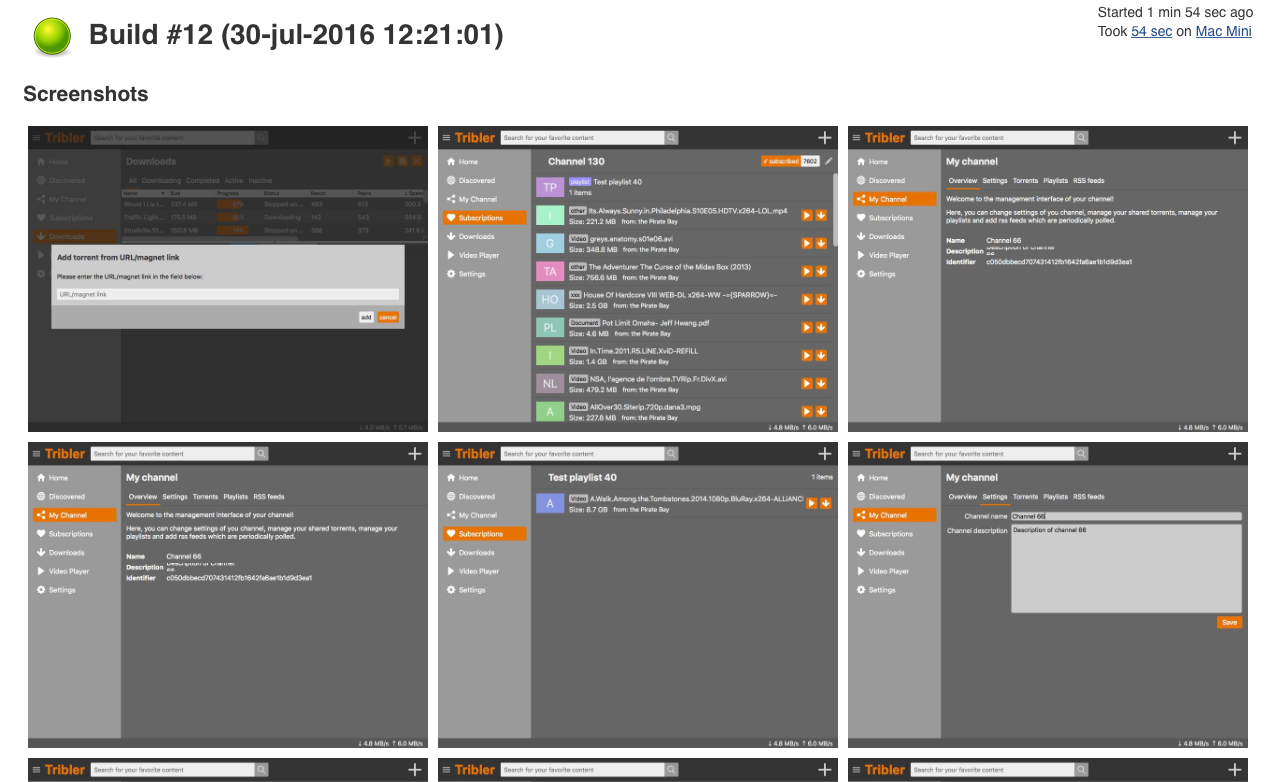
\includegraphics[width=1.0\columnwidth]{images/improving_qa/gallery_jenkins}
	\caption{The generated image gallery after executing of the user interface tests, generated by Jenkins.}
	\label{fig:jenkins-gallery}
\end{figure}

To avoid any dependency on core components of Tribler itself, we implemented a small piece of software that provides the same interface as the REST API implemented in Tribler. This 'fake' API is much simpler in nature and has a very simplistic in-memory data model. By utilizing this API, we are able to control API responses, significantly improving the predictability of the tests. The downside of this approach is that new endpoints have to be written twice, once in Tribler and once in this fake API. We should note that it takes less time to implement an endpoint in the fake API since it is more simple.\\\\
A summary of various statistics related to these GUI tests is displayed in Table \ref{table:gui-tests-summary}. We note that the average execution time per test is higher than the time presented in Table \ref{table:test-suite-improvements}, however, during the tests there are various situations where we have to wait for incoming data from the fake API provider. Starting the GUI and the Tribler core also takes several seconds.

\begin{lstlisting}[caption={An example of a test that tests the new Qt Tribler GUI.},label={lst:qtest-sample}]
def test_home_page_channels(self):
	QTest.mouseClick(window.left_menu_button_home, Qt.LeftButton)
	QTest.mouseClick(window.home_tab_channels_button, Qt.LeftButton)
	self.screenshot(window, name="home_page_channels_loading")
	self.wait_for_home_page_table_populated()
	self.screenshot(window, name="home_page_channels")
\end{lstlisting}

\begin{table}[h!]
	\centering
	\begin{tabular}{|l|l|}
		\hline
		\textbf{Amount of tests} & 23 \\ \hline
		\textbf{Total execution time on macOS} & 1 min. 4 sec. \\ \hline
		\textbf{Average execution time per test} & 2.8 sec.\\ \hline
	\end{tabular}
	\caption{A summary of statistics of the GUI tests.}
	\label{table:gui-tests-summary}
\end{table}

\subsection{External Network Resources}
\label{subsec:external-network-resources}
On of the identified code smells in Table \ref{table:tests-code-smells} is the dependencies on external resources, leading to unstable and unpredictable tests. To elaborate, the test suite contains various tests where external torrent files are fetched from the Internet, in particular, from the Ubuntu repository. While this repository guarantees a high availability, any downtime in this external resource leads to failing tests, failures not caused by code contributed by a specific developer. The implemented solution for this flaw is to start up a local HTTP server that serves the torrent file. While this approach requires additional code for management of a local web server, it completely removes the dependency on the Ubuntu repository, thus increasing reliability of our tests.\\\\
A similar solution has been applied to solve the dependency on seeders in the libtorrent network by setting up a local session that seeds a torrent. Again, this approach requires code to properly start and shut down the seeder session, thus increasing complexity of the test suite. However, the implementation is reusable to an extend that developers of tests can reuse the implemented solution with only a few lines of code.\\\\
Unfortunately, there are various external dependencies left which are considered harder to refactor. A handful of tests are performing a remote keyword search, requiring various communities in Dispersy to be available. These tests are dependent on available peers in the respective community in order to ensure incoming search results. Due to time constraints, getting rid of this dependency is considered future work.

\subsection{Instability of Tests}
\label{subsec:instability-tests}
An unstable testing suite has a direct impact on the productivity of developers: when tests fails to reasons unrelated to the code that the developer contributed in a specific commit, developers have to execute the test suite again. One method to do this is by writing a comment on the pull request (PR) on GitHub that says \emph{retest this please}. Every retest operation is "wasting" several minutes since developers have to wait for the completion of test execution before they have the necessary feedback about the stability of their PR. This is a structural problems that Tribler developers are experiencing since the utilization of continuous integration.\\\\
To further investigate this problem, we estimate the total time developers had to wait for retests by writing a small script that uses the GitHub API\footnote{https://developer.github.com/v3/} to analyse every opened PR and count the amount of retests required before the PR is merged into the main code base. Before we present the results, we should note that we might miss some occurrences since it is possible to remove comments on GitHub. In addition, some retests might be related to failures in the continuous integration environment and are not caused by flaws in the test suite. In total, we counted 2.045 retests in 1.481 pull requests, on average, 1.38 retests for each merged PR. If we use an optimistic estimation where an execution of the full test suite takes six minutes in total, we spent around 204 hours retesting pull requests. We argue that we can stabilize the test suite in much less time so we need less retests. To demonstrate that we are dealing with a structural problem here since 2013, the number of retests over time has been displayed in Figure \ref{fig:retest-this-please-required} where each vertical bar represents an individual PR. The vertical axis denotes the number of (manual) retests required before the PR got merged.\\

\begin{figure}[h!]
	\centering
	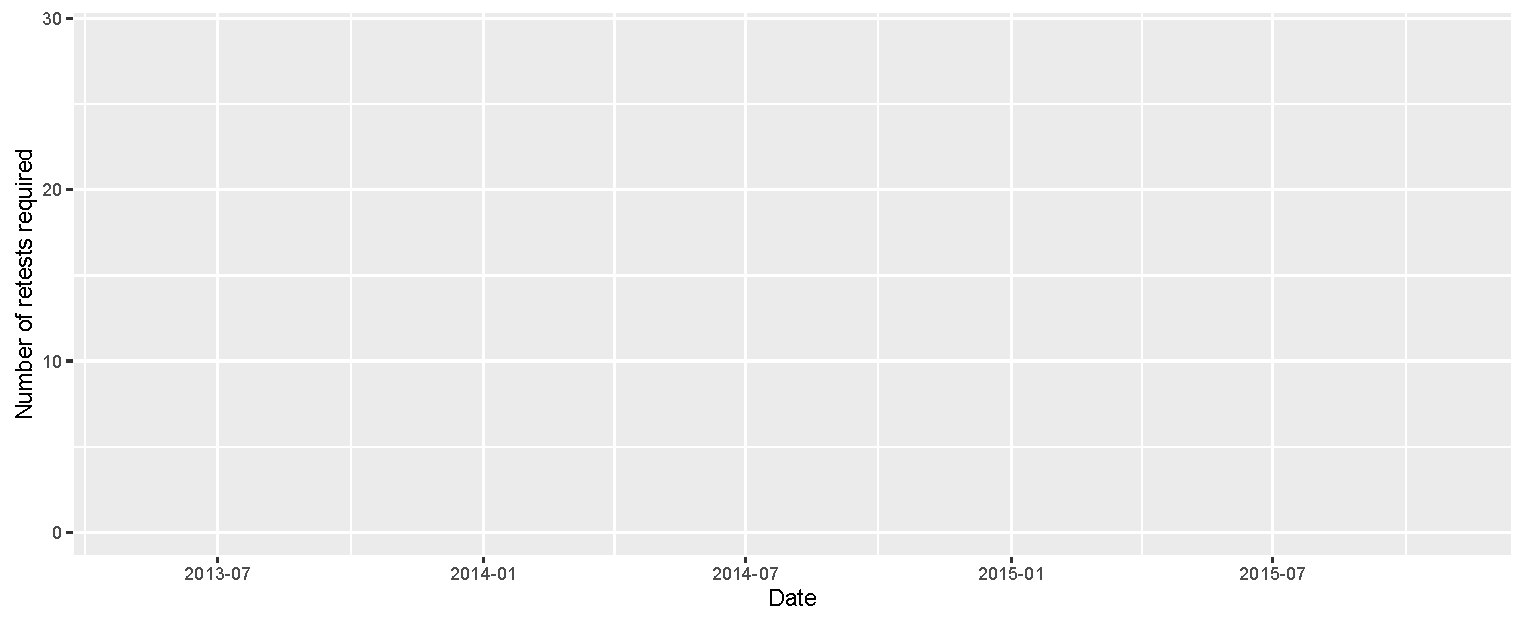
\includegraphics[width=1.0\columnwidth]{images/improving_qa/retests_required}
	\caption{The number of retests required in PRs over time.}
	\label{fig:retest-this-please-required}
\end{figure}

Essentially, we are dealing here with a special kind of technical debt: developers prudently made the decision to postpone fixing of the problems in the test suite by retesting the PR until the tests suite succeeds. The incentives to spent some time to fix test errors are not apparent and often, developers do not feel that they are responsible for failing tests since it might have been caused by code written by other developers. This makes it attractive to ignore test failures.\\\\
Well-designed tests should only fail if some new code is breaking existing functionality. If no changes are presents, the tests should always succeed, regardless of how many times they are executed. Reducing dependencies on external resources is not sufficient to guarantee this desired property. The structural problem of the tests is that the system is infected a great amount of race conditions. Race conditions can be hard to spot since they often occur in a very specific runtime setting, making the debugging process of these kind of errors frustrating. In fact, it is very easy to deliberately introduce a race conditions that is not noticed after the code is merged into the main branch. A complex architecture is directly influencing this phenomena and leads to more race conditions, possibly caused by wrong threading assumptions.\\\\
During this thesis, several race conditions have been detected and solved. One interesting observation is that some issues only occurred on a specific platform. We believe can be explained by differences in the implementation of underlying threading model and runtime architecture across operating systems. The most common origin of the detected race conditions is addressed to delayed calls in Twisted. During the test execution a Tribler session is started several times. If a developer leaves a delayed call behind when the shut down procedure has been completed, this delayed call might be executed in another Tribler session, possibly leading to an inconsistent state of the system. Making sure Twisted is void of any delayed call is not straightforward: if one is not aware of scheduled calls in the system, this mistake is easily made.

\section{Infrastructure Debt}
Tribler uses of the popular CI platform Jenkins\footnote{https://jenkins.io}. Jenkins allows developers to create jobs which can be executed manually or when pushing a commit on the code base. The CI platform is responsible for running the tests, packaging Tribler and executing research-oriented experiments on the DAS5 supercomputer.\\\\
We noticed that the test suite is only executed in a Linux environment. Beller et al\cite{beller2016oops} conducted research on CI adoption and usage and it turned out that for some languages, it might benefit to run tests in different environment. We strongly agree with this vision and since Tribler is shipped for multiple platforms, we think it is of uppermost importance to run the unit tests in different environment. An addition argument for this is the presence of some platform-specific workarounds: to make sure that these statements are covered by the tests, we must run the test suite in the specific environment. This will allow developers to detect defects on other platforms more earlier in the development process. By aggregating the generated coverage report on each platform, this multi-platform set-up should have a (small) positive influence on the code coverage metric.\\\\
The set-up of the testing environments on Windows and macOS is straightforward: new slave nodes to specify the Windows and macOS test runners have been created in Jenkins. The tests on macOS are executed on a Mac Mini, late 2014 model with 4GB of DDR3 memory and an Intel Core I5 1.4 GHz processor. In order to run the tests on Windows, two virtual machines using Proxmox\footnote{https://www.proxmox.com}, a server virtualization management platform, have been created, both with 32-bit and 64-bit environments. After the utilization of these additional machines, the tests are executed on four platforms: Linux, 32-bit and 64-bit Windows and macOS. So far, both the macOS and Windows test executers have completed over 2.700 test executions. Each test runner generates a coverage report and all reports are merged in the final analysis step in the build pipeline.

\subsection{Future Improvements}
While multi-platform test execution is certainly a step in the right direction, there are additional steps in the execution plan that could enhance the testing procedure. In Figure \ref{fig:jenkins-pipeline}, we present what we think is the ideal test execution plan, together with various stages in this pipeline. The dashed boxes are jobs in the pipeline that are not implemented yet. The Jenkins job is triggered by a commit on GitHub and starts with the execution of the tests on multiple platforms where during these runs, code coverage is being tracked. After this phase, the coverage reports are combined and the total difference with the upstream branch is determined. When the commit decreases the total code coverage, the job fails and the pipeline aborts. This negative result is presented in the PR on GitHub.\\

\begin{figure}[h!]
	\centering
	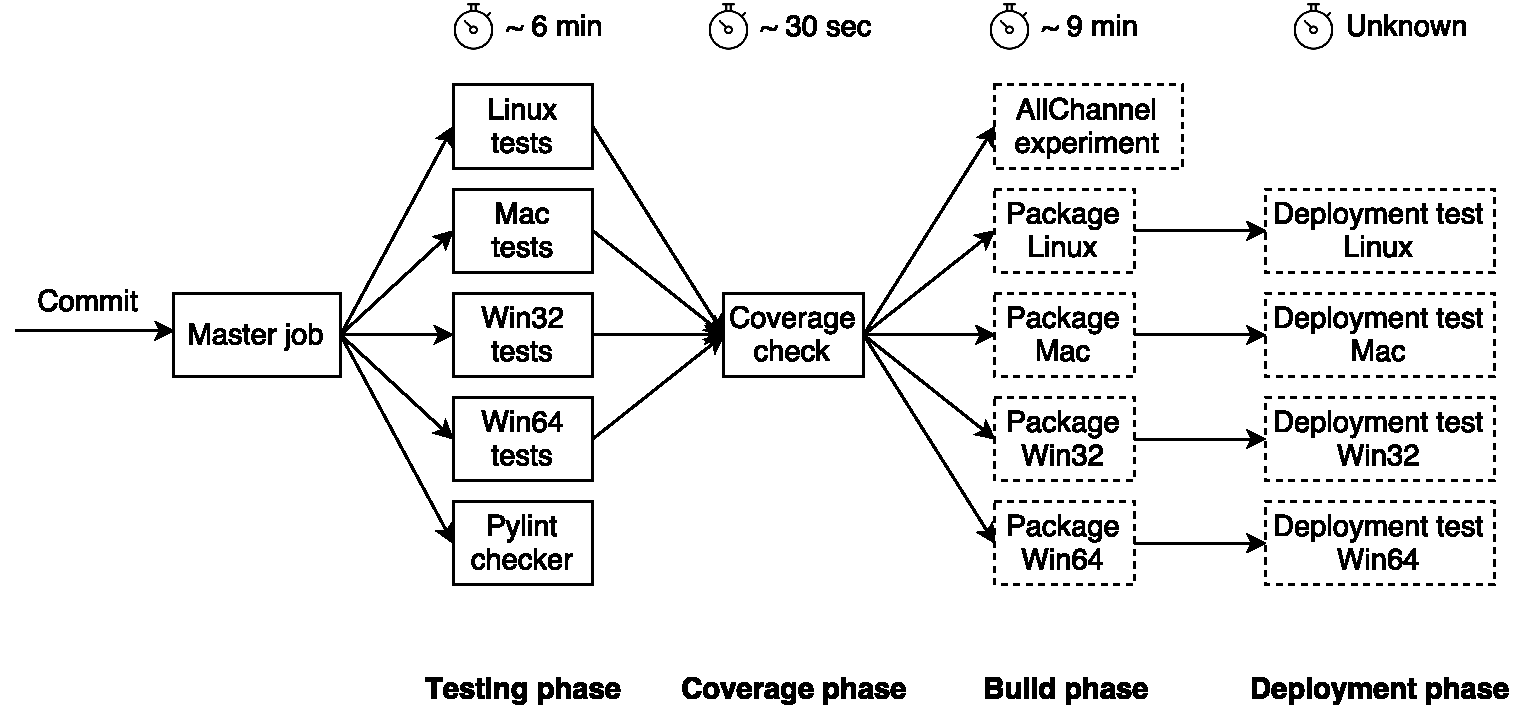
\includegraphics[width=0.9\columnwidth]{images/improving_qa/jenkins_pipeline}
	\caption{The desired test execution plan in our CI environment. Dashed boxes are Jenkins jobs that are not implemented yet.}
	\label{fig:jenkins-pipeline}
\end{figure}

A static Pylint\footnote{https://www.pylint.org} checker to check for code style violations has been available for a long time, however this only gave insight in the total amount of Pylint errors in the whole code base and did not stimulate to actually fix errors in the committed code of a developer. While not implemented by the author of this thesis, the Pylint checker has been extended to fail if new violations are introduced in committed code. Additionally, a report is generated with an overview of the introduced violations, together with the relevant source code. This helps developers to get more aware of their code style and helps to realise a consistent code base. This check is executed in parallel with the tests to decrease the total time of the pipeline execution.\\\\
After the coverage phase has passed, the AllChannel experiment should be performed. This experiment is executed on the DAS5 supercomputer and starts 1.000 Tribler clients that are synchronizing torrent and channel information with each other. When the experiment is completed, various graphs are generated. Examples of these graphs includes the number of connections, the amount of messages synchronized and the number of invalid messages sent. These graphs provides developers insights in the performance of their modified code when Tribler runs in a large-scale setting. For instance, the experiment can highlight introduced issues in the message synchronization between peers in the network.\\\\
In parallel with the AllChannel experiment, we should package Tribler for distribution to end-users. An additional purpose of this step is the execution of deployment tests on various platforms to check whether Tribler works when being distributed to end users. On Windows, an installer will be created that installs Tribler to the \emph{Program Files} directory. On macOS, we create a \emph{.dmg} file that contains an app bundle. On Linux, the required files are bundled in a \emph{.deb} archive. Packaging and deployment testing jobs can be executed in parallel to shorten the time of the testing pipeline as visible in Figure \ref{fig:jenkins-pipeline}.

\section{Architectural Debt}
Already indicated by Figure \ref{fig:wx-import-graph} in Chapter \ref{chapter:problem-description}, Tribler is plagued with many dependencies that are leading to a highly coupled system where it is hard to reuse individual components. We aim for a low coupling to increase testability of packages. This section will focus on identification and removal of undesired dependencies between packages.

\begin{figure}[h!]
	\centering
	\begin{subfigure}{.5\textwidth}
		\centering
		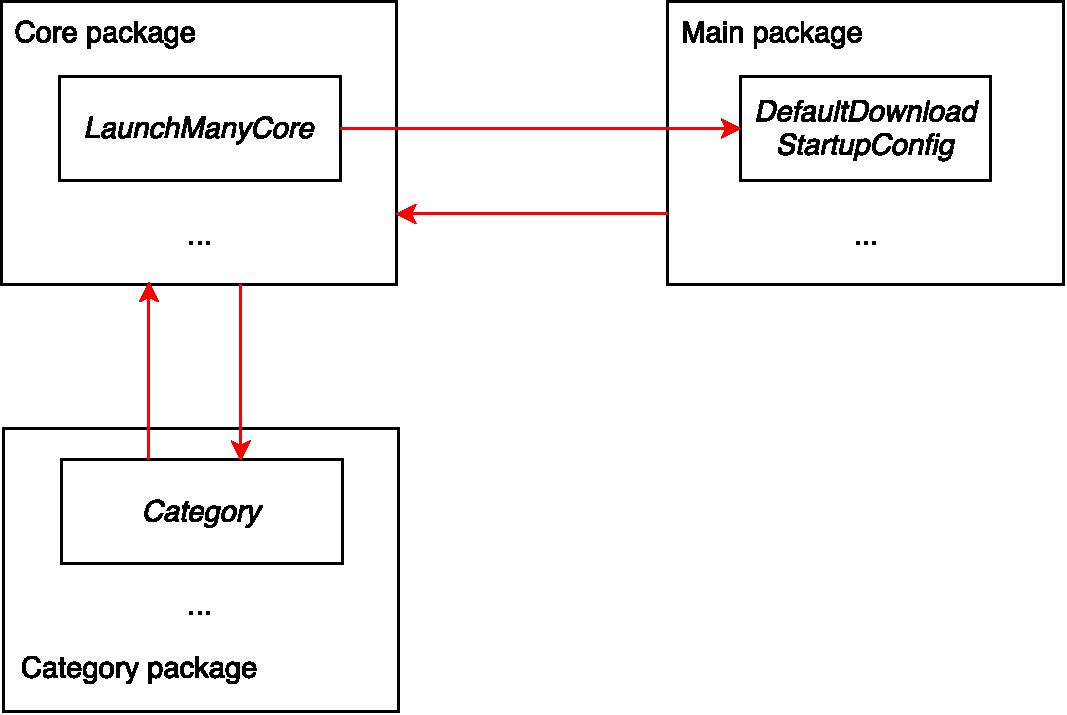
\includegraphics[width=0.9\linewidth]{images/improving_qa/cycle_tribler_package}
		\caption{Before refactoring}
		\label{fig:tribler-packages-refactoring-before}
	\end{subfigure}%
	\begin{subfigure}{.5\textwidth}
		\centering
		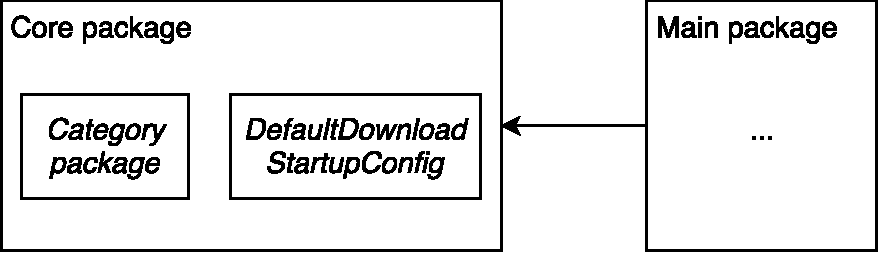
\includegraphics[width=0.9\linewidth]{images/improving_qa/cycle_tribler_package_after}
		\caption{After refactoring}
		\label{fig:tribler-packages-refactoring-after}
	\end{subfigure}
	\caption{The dependencies between Tribler modules at the highest level. Cyclic import dependencies are shown in red.}
	\label{fig:tribler-packages-refactor}
\end{figure}

\subsection{GUI and Core Dependencies}
\label{subsec:gui-core-packages}
As described in Chapter \ref{chapter:problem-description}, the source code for the user interface and Tribler core code is interleaved to a large extent and there is no clear separation between those two. There are various instances where we identified code present in the GUI code base that should be moved to the core and vice versa. To realise a clear separation between libtribler and the user interface, we should make sure that we move code to the package where it belongs.\\\\
In the present code base, the \emph{Core} package is dependent on the user interface which is undesired: we are unable to utilize the Tribler core without the GUI code being present, leading to high coupling. The exact dependency is visible in Figure \ref{fig:tribler-packages-refactoring-before} and is caused by the \emph{DefaultDownloadStartupConfig} class which is located in the \emph{globals.py} file, part of the GUI package. This class is responsible for providing default configuration options when a download is being started, in case the user did not override default options like the destination of the downloaded file and the amount of anonymous hops used during the download. Since the superclass of \emph{DefaultDownloadStartupConfig}, \emph{DownloadStartupConfig}, is already located in the Tribler core, it makes sense to move the \emph{DefaultDownloadStartupConfig} class to the \emph{DownloadConfig.py} file, which already contains the \emph{DownloadStartupConfig} class. After we moved this class to the core and modified the references to point to the new location of the class, the core is completely independent of the user interface, displayed in Figure \ref{fig:tribler-packages-refactoring-after}.

\subsection{Category Package}
Referring to Figure \ref{fig:tribler-packages-refactor}, we note a cyclic import dependency between the \emph{Core} and \emph{Category} package. The \emph{Category} package hosts the source code to facilitate the family filter. Obviously, the family filter is used by the Tribler core, however, the family filter also has dependencies on classes inside the Tribler core, leading to a cyclic import.\\\\
In the architecture proposed in Figure \ref{fig:tribler7}, we specified the family filter as a component of libtribler. We think that the best solution to solve this dependency, is to move the \emph{Category} package to the Core package so it's part of libtribler. This change is reflected in Figure \ref{fig:tribler-packages-refactoring-after}.

\subsection{Video Player}
We will now zoom in on the core package which contains some GUI-related code that should not be present in that package. The most obvious occurrence is attributed to management of the (embedded) video player in Tribler which is handled by the \emph{VideoPlayer} class in the \emph{Video} package. Figure \ref{fig:video-package-refactoring-before} shows the import graph of the \emph{Video} package before refactoring. The \emph{VideoPlayer} class makes use of the VLC bindings for Python, however, in our design, the core does not need to have any dependency on VLC since managing the video player is an operation that should be performed on the level of the user interface. The \emph{LaunchManyCore} class (not part of the \emph{Video} package) contains code to initialize all components available in Tribler, including the \emph{VideoPlayer}. When initialized, this \emph{VideoPlayer} creates a \emph{VideoServer} that is responsible for the streaming capabilities of Tribler. Finally, the \emph{VLCWrapper} class contains various utility methods to work with raw VLC data such as the time position within a video.\\\\
We performed refactoring work within this package and removed the \emph{VideoPlayer} and \emph{VLCWrapper} classes. The composition of the \emph{Video} package after this operation is displayed in Figure \ref{fig:video-package-refactoring-after}. We modified the code so the \emph{LaunchManyCore} class starts a video server instead of a video player. We point out that there are some classes that are unused now, such as \emph{VideoUtility} and \emph{utils}: these classes contains various helper methods to retrieve thumbnail images from a video file and is considered legacy code. Due to time constraints, we are unable to implement these features in the new user interface so for the time being, we keep these files as reference for future development.

\begin{figure}
	\centering
	\begin{subfigure}{.5\textwidth}
		\centering
		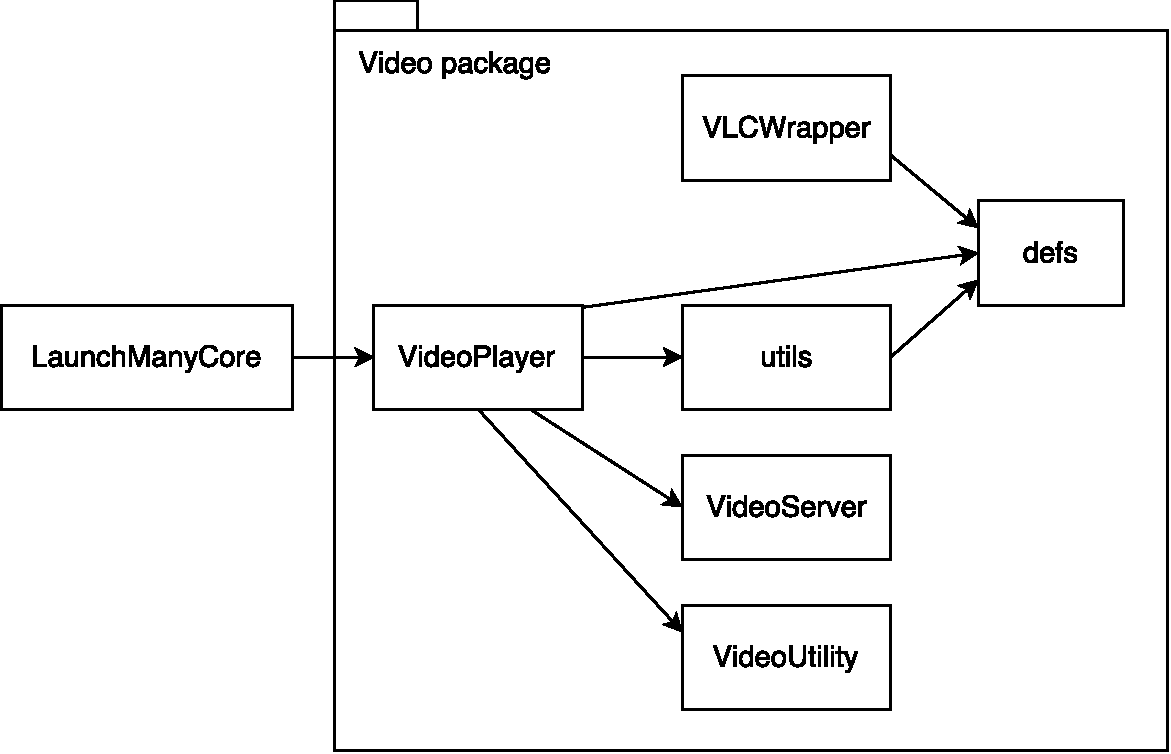
\includegraphics[width=.9\linewidth]{images/improving_qa/video_package_before}
		\caption{Before refactoring}
		\label{fig:video-package-refactoring-before}
	\end{subfigure}%
	\begin{subfigure}{.5\textwidth}
		\centering
		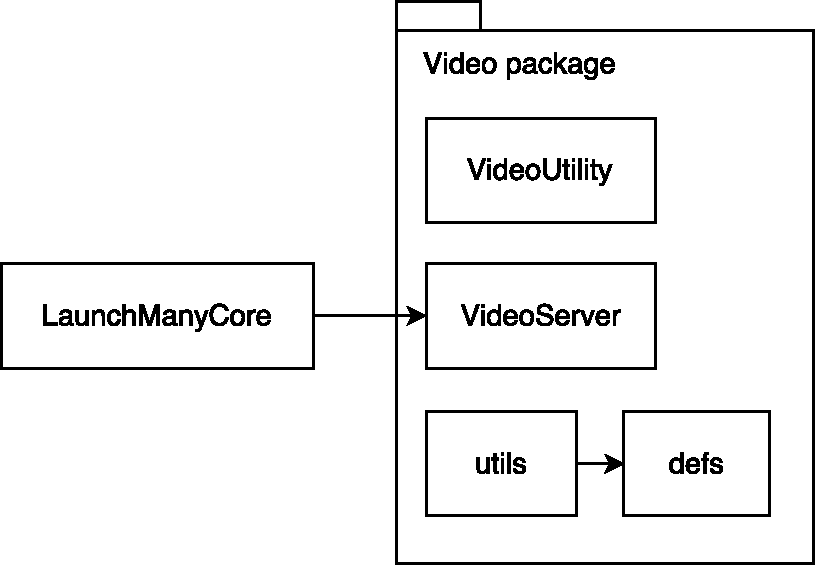
\includegraphics[width=.7\linewidth]{images/improving_qa/video_package_after}
		\caption{After refactoring}
		\label{fig:video-package-refactoring-after}
	\end{subfigure}
	\caption{The import graph of the \emph{Video} package and the \emph{LaunchManyCore} file in the Tribler core before and after refactoring.}
	\label{fig:video-package-refactoring}
\end{figure}

%\section{Updating software dependencies}
%A cause of ageing software is the inability of developers to adopt to changing environment. This might be addressed to adoption of dependencies in the past, dependencies that are not maintained any more at a point in the future. Replacing these dependencies might be a non-trivial programming task, requiring the programmer to get familiar with both the interface of the old and new dependency.\\\\
%Tribler has a long list of dependencies, both in the code base and dependencies that are used for software packaging and testing. Keeping these dependencies on the latest version is often neglected or overlooked. Sometimes, this is not even possible, due to missing software in package managers such as \emph{yum}, the package manager used by CentOS or \emph{apt}, the package manager of Debian and Ubuntu. While this restriction holds for operating systems where we are not packaging dependencies, we have the freedom to package any dependency we want on Windows and macOS so preferably, we often want to ship the latest, stable release of a dependency in our Tribler distribution.\\\\
%During this thesis, we updated several dependencies to newer versions, most notably \emph{libtorrent}. The code to handle the communication with this library (located in the \emph{Libtorrent} package) contained calls to deprecated functions in the \emph{libtorrent} library, functions that are not guaranteed to be maintained or compatible. We identified these calls as follows: first, a version of \emph{libtorrent} has been compiled without deprecated methods and assertions. Next, we manually ran Tribler and the test suite, observing any crash due to libtorrent. In total, this method yielded seven calls to deprecated methods that have been updated to call the correct function. Not only deprecated calls have been removed, we also fixed various assertions that were triggering due to incorrect assumptions made in the code. In order to remain backwards-compatible with older version of the libtorrent library (that some Ubuntu or Debian users might have installed on their system), some checks in the Tribler code base had to be implemented to check for the presence of a particular method in libtorrent.\\\\
%An additional outdated dependency in Tribler is \emph{py2exe}, used to create a Windows executable file out of the source code. \emph{py2exe} performs a static code analysis and determines code dependencies that should be bundled in the executable. Unfortunately, the library has not been updated since 2014 and requires a significant amount of code to make sure that everything works when Tribler is packaged and archived. We made attempts to replace \emph{py2exe} with the more mature, well-maintained \emph{PyInstaller} that also offers support for \emph{PyQt5}, the framework used for creation of the new interface. This library is not only easier to use, it also works across multiple platforms, allowing us to also drop the \emph{py2app} dependency which is used to distribute Tribler on macOS. While not ready for deployment yet, a proof-of-concept has been created that successfully packages Tribler together with the new user interface into Windows and macOS executable files. Further work should focus on the removal of \emph{py2exe} and \emph{py2app} in favour of \emph{PyInstaller}.

\section{Documentation Debt}
\label{sec:software-artifacts}
During the last years of development efforts on Tribler, the main focus of the project has been to deliver working code. The project has a severe lack of updated software artifacts, including documentation, code comments and architectural diagrams, leading to a huge amount of \emph{documentation debt}. Some of the conducted research was documented on the Tribler wiki\footnote{https://www.tribler.org/TitleIndex/}, however, this wiki contains many outdated pages and is not used or maintained anymore. After the migration of the project to GitHub, this platform was favoured for storing documentation over continued usage of the Tribler wiki archive. A good documentation helps to get new developers familiar with the system but also helps to prevent software ageing\cite{parnas1994software}, the situation where it gets harder for software to meet requirements over time.\\\\
Currently, there are distinct locations where we store the few software artifacts we have. Documentation is either stored in the GitHub wiki, in the wiki on the Tribler website or in the \emph{docs} directory in the Tribler source code repository. The ideal situation is to have one single location for all generated software artifacts during the process. Many Python projects are using readthedocs\footnote{https://readthedocs.org}, a platform to host documentation of open-source projects for free. The hosted documentation should be located in the Tribler source code repository, in \emph{reStructuredText} (RST) format. By utilizing the Python module Sphinx, a website can be generated from all the available documentation. Sphinx also provides possibilities for translation of documentation in other languages.\\

\begin{figure}[h!]
	\centering
	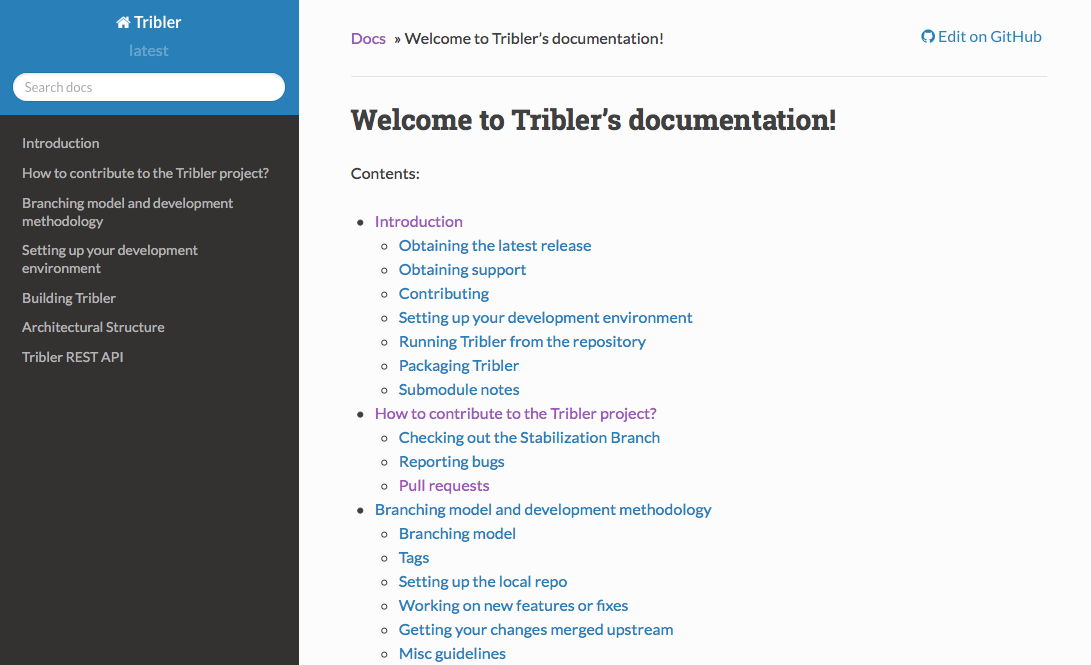
\includegraphics[width=1.0\columnwidth]{images/improving_qa/readthedocs}
	\caption{The new documentation base of Tribler, as available on the \emph{readthedocs} website.}
	\label{fig:documentation-tribler}
\end{figure}

During this thesis, all available documentation of Tribler has been rewritten in RST format in conjunction with Sphinx. Moreover, the available documentation has been expanded with several guides, in particular, guides that help new developers to set-up an environment on their machine. Prior to this thesis, these guides were not available and development on other platforms than Linux was not supported. By the addition of these guides, new developers can start as soon as possible with Tribler development. The website with documentation of Tribler is visible in Figure \ref{fig:documentation-tribler} and is available on the readthedocs website\footnote{http://tribler.readthedocs.io/en/latest/}.\\\\
In particular, the REST API has been well documented. Since external developers should use the REST API to control and get information from Tribler, we wish to provide a clear and comprehensive documentation base for this API. To simplify the process of writing documentation, the documentation can be written as doc strings above each method in the source code. This documentation is parsed by the autosummary tool\footnote{http://www.sphinx-doc.org/en/stable/ext/autosummary.html} that is executed each time the documentation is built: it navigates through the API code base, extracts all doc strings and generates separate sections for each annotated method. The doc string can be attributed with \emph{RST} syntax. This feature decreases chances that developers accidentally forget to write or update artifacts since the code and documentation is present in the same file instead of being spread across different distinct files.

\section{Preventing Technical Debt}
Prevention is the best medicine and we must think about a change in the development process that prevents technical debt in the future. Developers have never been aware of the long-term consequences of the Tribler architecture and their work. To stop the deterioration of the system, we must raise awareness of technical debt and the term needs to play a more profound role when making long-term development decisions. To realise this, we present the following list of implemented ways to raise technical debt awareness:
\begin{itemize}
	\item Introducing mandatory code reviews of new PRs is an effective way of ensuring that problems in the code are detected as early as possible\cite{18fpreventdebt} but additionally, it helps developers to learn from their mistakes and to raise the quality bar of contributed code. The new policy introduced during this thesis requires each PR of developers to be reviewed by at least two other Tribler developers. This policy also helps developers to get more aware of ongoing work performed by other developers.
	\item Continuous integration and automated testing is an excellent opportunity to maintain a higher level of code quality and to catch bugs during the development process before end users are reporting them. The work as described in this chapter, has matured the Jenkins and testing environment so it can be used reliably by the next generation of Tribler developers.
	\item Our CI environment already used static analysis tools to report violations in the source code which is an effective way to make developers aware of their introduced violations\cite{nagappan2005static}. However, when starting this thesis, these analysis tools have been implemented as separate jobs and were not executed on every pull request. This has been changed so developers receive fast feedback when they push a new commit to GitHub. The implemented checks executed for every PR on GitHub are visible in Figure \ref{fig:jenkins-check}. Besides the reports of the test execution on multiple platforms and the code violation reporter, the code coverage report fails if developers added or modified lines that are not covered by a test. This tool will definitely contributes towards an increase of the code coverage metric in the long run. The code style violation checker will help us to prevent the amount of code smells identified by the static code analyser.
\end{itemize}

\begin{figure}[h!]
	\centering
	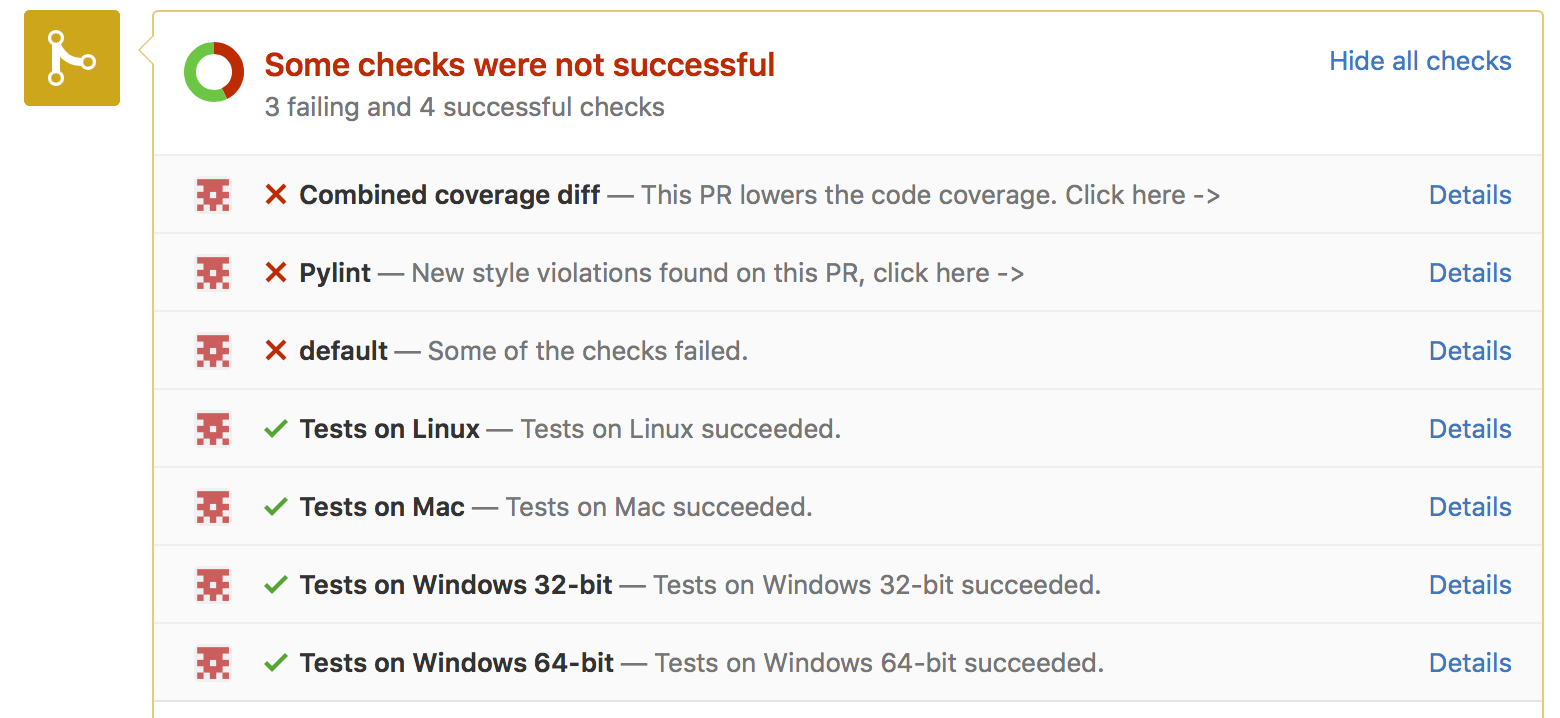
\includegraphics[width=1.0\columnwidth]{images/improving_qa/jenkins_checks}
	\caption{The implemented checks in Jenkins, executed on every new commit in a PR.}
	\label{fig:jenkins-check}
\end{figure}
\chapter{Performance Evaluation of libtribler}
\label{chapter:experiments}

Technical debt has a negative impact on product quality in terms of defects and other structural quality issues\cite{tom2013exploration}: it is significantly harder to fix defects in a complex, unstructured system and more dangerous in a sense that one might introduce additional bugs when trying to solve one. Boosting performance is often achieved by minor or major refactoring efforts of system components to utilize another underlying model or structure. Modifications of the system is more involved when the system as whole is suffering from huge amounts of technical debt.\\\\
Now that we got rid of most of the technical debt identified in the Tribler core, the next step towards a stable, future-proof libtribler involves research efforts on the usability and performance of various components. We wish to quantify the performance of operation in libtribler to get an idea about the usability of the core in general. For various components in the core, we have no performance baseline to help us to make statements about usability. We will perform a number of experiments and for each experiment, we will present and discuss the observed results. The underlying reason for this experiment is twofold: on the one hand, we show that the performance of the system did not degrade to an  unacceptable extent due to our refactoring efforts. On the other hand, we use the performance measurements to create a baseline and to identify possible failures or issues that we will classify as future work.

\section{Environment Specifications}
The experiments performed in this Chapter are executed on a \emph{virtual private server (VPS)}. We wish to stay as close as possible to the specifications of a machine that an actual user could be using. A summary of the specifications of the machine used for most of the experiments described in this Chapter, is given in Table \ref{table:experiments-server-specifications}.

\begin{table}[h!]
	\centering
	\begin{tabular}{|l|l|}
		\hline
		\emph{CPU} & Intel Xeon CPU E5-2450 (2.50GHz, 4 cores)\\ \hline
		\emph{Memory} & 8GB 1000MHz \\ \hline
		\emph{Hard disk} & 50GB \\ \hline
		\emph{Operating system} & Ubuntu 15.10 \\ \hline
	\end{tabular}
	\caption{The specifications of the machine used for most of the experiments.}
	\label{table:experiments-server-specifications}
\end{table}

The experiments are not executed in an isolated, artificial environment but instead in the wild, using the deployed Dispersy network. While the obtained results may be different between users, this set up can be used to get more insights in the performance of Tribler from a user's perspective.\\\\
If not stated otherwise, the default Tribler configuration file values are used. These default values can be found in the \emph{defaults.py} file in the source code directory of Tribler\footnote{https://github.com/Tribler/tribler/blob/devel/Tribler/Core/defaults.py}. In this configuration file, all communities, except for the \emph{BarterCast} community, are initialized. Dispersy, the HTTP API and the video server are enabled during the experiments. All experiments are executed without running the \emph{wxPython} or Qt GUI.\\\\
Some of the experiments are built using a scenario file. In such a scenario file each line specifies a specific command of a peer at a specific point in time during the experiment. Our framework to run the experiments, Gumby, contains code to read scenario files, interprets the commands to be executed and to schedule these commands in Twisted. Several utility methods have been implemented to gather and write statistics to files in a processable and readable format that can be parsed by visualization tools such as \emph{R}\footnote{https://www.r-project.org}. Various Dispersy experiments are already using the scenario file framework, mainly in our \emph{AllChannel} experiment that runs on the DAS5 supercomputer. Before we executed the experiments in this Chapter, we first extended the usability of the scenario files to run and manage a Tribler session and we improved the framework with the addition of various commands to support the operations that are executed in the performed experiments in this Chapter. An overview of all implemented commands can be found in Appendix \ref{appendix:gumby-scenario-commands}. The flexibility of these scenario files gives developers a robust framework to use when conducting performance analysis, benchmarking and other kinds of scientific research with Tribler.

\section{Profiling Tribler on Low-end Devices}
\label{sec:profiling_tribler_lowend}
The implementation of a RESTful API gives developers a possibility to run and control Tribler from remote devices. For instance, one can run Tribler on a low-end, cheap devices such as a Raspberry Pi and use it to accumulate reputation in the Multichain by enabling the credit mining mechanism. Android is another example of a device that can run Tribler and during the last years, various research have been conducted to explore the possibilities of Tribler on Android devices\cite{sabee2014tribler}\cite{de2014android}. Executing and profiling Tribler on a low-end device with limited resources can yield much information about bottlenecks that might not be directly visible when running Tribler on a regular desktop or supercomputer.\\\\
The experiments described in this Section are all executed on a Raspberry Pi, third generation with 1GB LPDDR2 RAM, ARM Cortex-A53 CPU with 4 cores, a 1.2GHz CPU and 16GB storage on a microSD card. The installed operating system is Raspbian, an operating system specifically designed for the Raspberry Pi and derived from Debian, an operating system suitable for desktops.\\\\
Some preliminary exploration of the performance on the Raspberry Pi using the REST API has us suspected that the device is under heavy load when running Tribler. Monitoring the process for a while using the \emph{top} tool, reveals that the CPU usage is often around 100\%, completely filling up one CPU core. To get a detailed breakdown of execution time per method in the code base, the Yappi profiler has been used to gather statistics about the execution time of methods in Tribler. This profiler has been integrated in the \emph{twistd} plugin and can be started together with Tribler by passing an option. The output generated by the profiler is a \emph{callgrind} file that should be loaded and analysed by third party software. The breakdown of a 20-minute run is visible in Figure \ref{fig:yappi_breakdown}. This breakdown is generated using \emph{QCacheGrind}\footnote{https://sourceforge.net/projects/qcachegrindwin/}, a \emph{callgrind} file visualizer. We start this experiment with a clean state directory which is equivalent to the first boot of Tribler.

\begin{figure}[!h]
	\centering
	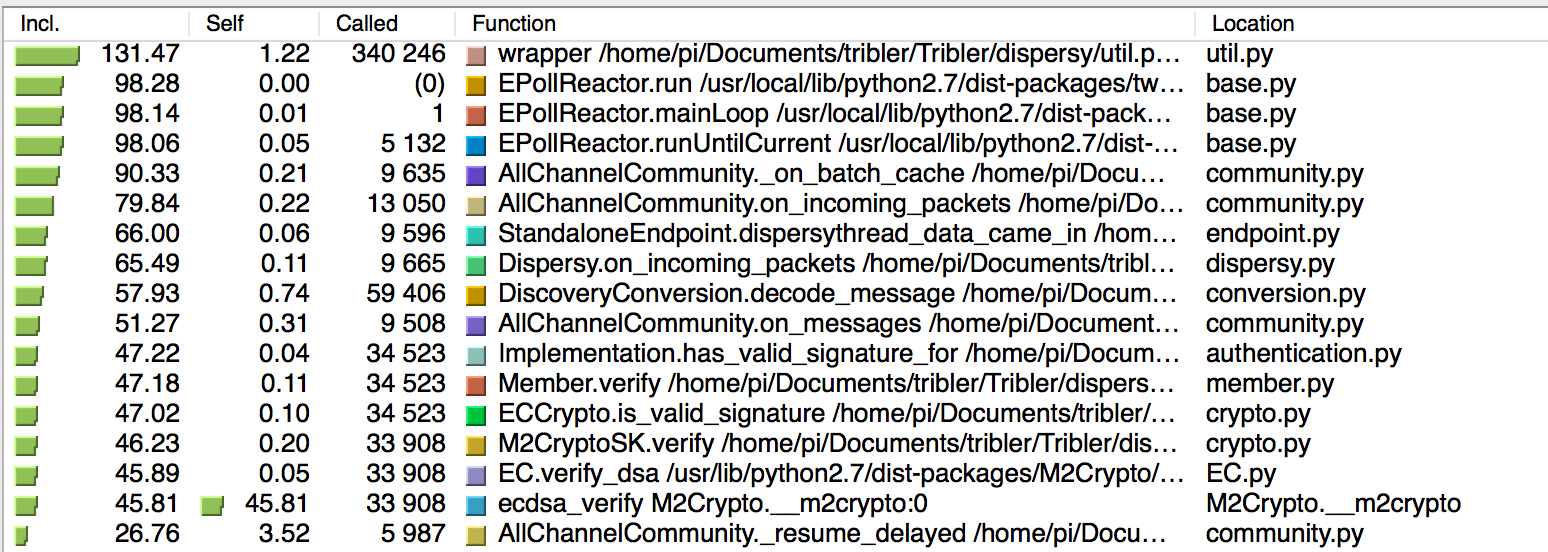
\includegraphics[width=1.0\columnwidth]{images/experiments/yappi_breakdown}
	\caption{The breakdown of a 20-minute run of Tribler on the Raspberry Pi.}
	\label{fig:yappi_breakdown}
\end{figure}

The file created by the Yappi profiler provides a detailed overview of the execution time of methods in Tribler and can be used as a tool to detect performance bottlenecks in the system. Referring to Figure \ref{fig:yappi_breakdown}, the column \emph{Incl.} denotes the inclusive cost of the function, in other words, the execution time of function itself and all the functions it calls. The column \emph{self} denotes only the execution time of the function itself, without considering callees. The other columns are self-explanatory and could be used to locate the respective function in the Tribler code base.\\\\
If we analyse the breakdown, we notice that Dispersy has a big impact on the performance of Tribler when running on the Raspberry Pi. The \emph{ecdsa\_verify} method (second method from the bottom) is dominating the runtime of Tribler: 45.81\% of the Tribler run time is spent inside this method. This specific method verifies the signature of an incoming Dispersy message and is invoked every time a signed message is received. Disabling cryptographic verification of incoming messages should improve the situation, however, this is a trade-off between security and performance: by not verifying incoming messages, fake messages by an adversary can be forged and are accepted in such a system.\\\\
To verify whether the system load when running Tribler decreases when we disable cryptographic verification of incoming messages, we measure the CPU usage of two different runs. Both runs start with a non-existing Tribler state directory and have a duration of ten minutes. In the first run, we are using the default configuration of Tribler, like in most of the other experiments described in this Chapter. In the second run, we disable verification of incoming messages in Dispersy. The CPU utilization over time of the two runs are displayed in Figure \ref{fig:raspi_cpu_usage}: on the horizontal axis, we show the time into the experiment and on the vertical axis, we display the CPU utilization in percentage. We emphasize that Tribler is limited to run on a single CPU core.\\\\

\begin{figure}[!h]
	\centering
	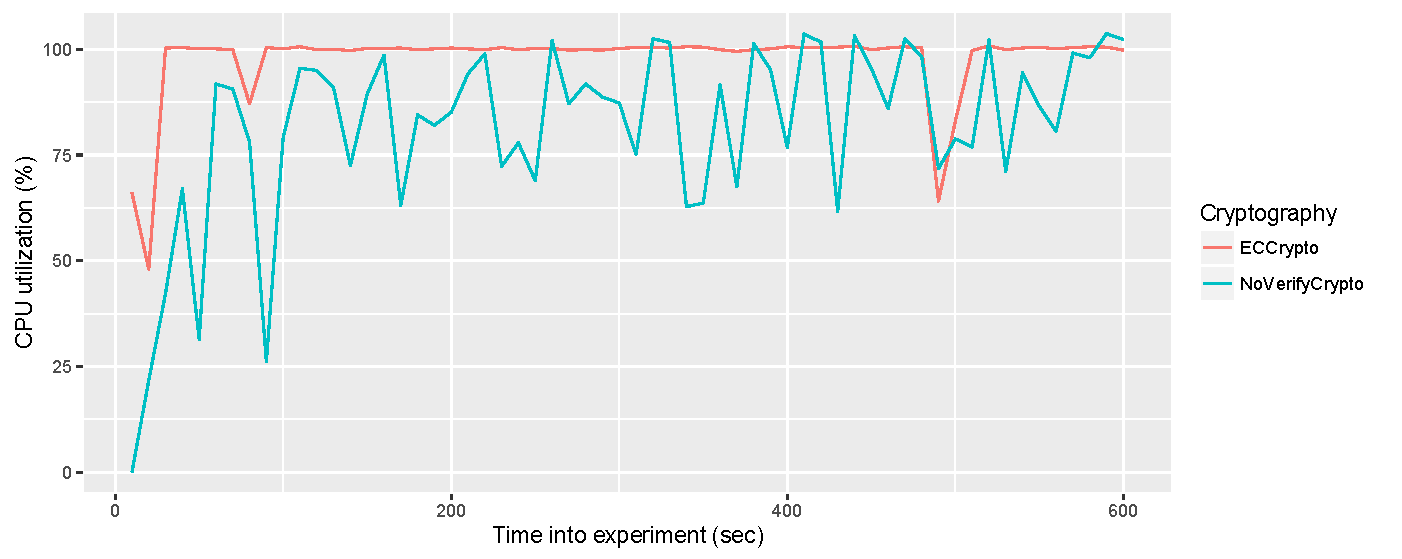
\includegraphics[width=1.0\columnwidth]{images/experiments/raspi_cpu_usage}
	\caption{The CPU utilization of one core on a Raspberry Pi device when running Tribler with and without cryptographic verification of incoming Dispersy messages.}
	\label{fig:raspi_cpu_usage}
\end{figure}

In Figure \ref{fig:raspi_cpu_usage}, some occurrences can be identified where the CPU usage appears to be slightly over 100\%. This is explained by the fact that some of the underlying code is designed to run on multiple processors. While the threading model of Tribler is limited to a single core, the Python interpreter might execute code on additional cores to improve performance. In the run where we enable cryptographic verification of incoming messages, the CPU usage is often 100\%, leading to a non-responsive system. When we disable message verification, we observe a somewhat lower CPU usage but overall, this utilization is still relatively high. Unfortunately, disabling incoming message verification is not enough to always guarantee a more usable and responsive system.\\\\
To detect other performance bottlenecks, we sort the report that has been generated by the Yappi profiler on the \emph{self} column to get insights in methods that are taking a long time to complete. This is visible in Figure \ref{fig:yappi_breakdown_self}. An interesting observation is that the Python built-in \emph{all} method takes up a significant amount of time (6.13\% of the runtime). The \emph{all} method takes an iterable object and returns \emph{true} if all objects of this collections resolve to a true value. Both the \emph{all} method and \emph{zip} method (also visible in Figure \ref{fig:yappi_breakdown_self}) is used in the \emph{\_resume\_delayed} method, indicating that this method might causing performance issues. Since further analysis of this method requires more knowledge of Dispersy, analysis and optimization of this method is considered future work and has been documented in GitHub issue 505\footnote{https://github.com/Tribler/dispersy/issues/505}.\\\\

\begin{figure}[!h]
	\centering
	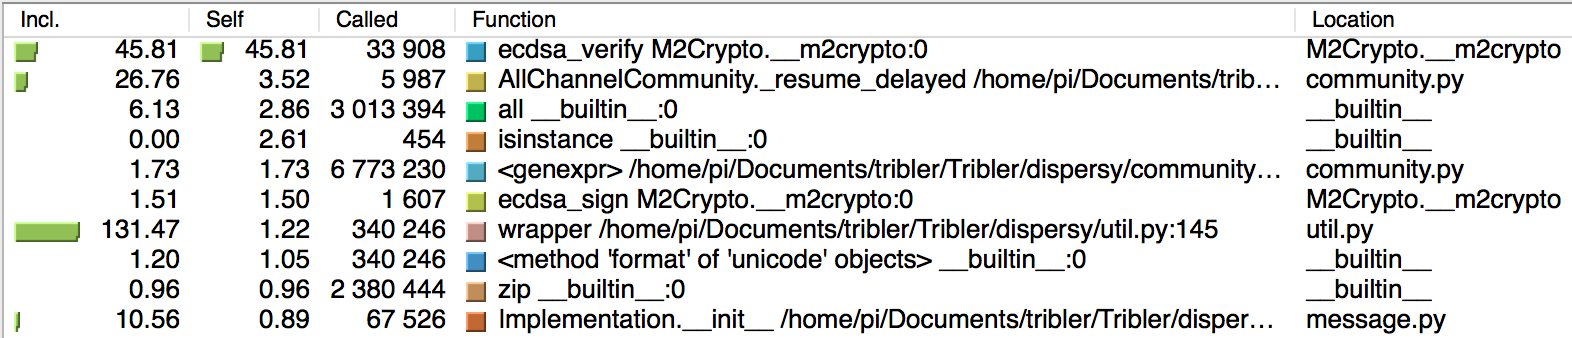
\includegraphics[width=1.0\columnwidth]{images/experiments/yappi_breakdown_self}
	\caption{The breakdown of a 20-minute run of Tribler on the Raspberry Pi, sorted on the \emph{Self} column.}
	\label{fig:yappi_breakdown_self}
\end{figure}

To summarize, we demonstrated how adequate usage the Yappi profiler can lead to the detection of performance bottlenecks present in Tribler and Dispersy. Integration of the profiler in the twistd plugin makes it convenient for developers to run and analyse Tribler sessions under different circumstances and on a broad range of devices.

\section{Performance of the REST API}
The responsiveness of the REST API is directly influencing the user experience. If the response times of API calls is high, users of Tribler have to wait longer before their data is available and visible in the user interface. For this reason, we wish to make the API serve requests as fast as possible. The purpose of this section is to assess the performance of the API with a particular focus on latency of request response times. However, some other statistics will be considered such as average request time, standard deviation of the response times and observed bandwidth. These statistics will help us to get more insights in the performance of the REST API and the responsiveness of Tribler.\\\\
We make use of Apache JMeter\footnote{http://jmeter.apache.org} that is used to perform HTTP requests to Tribler and to gather and process performance statistics. The application allows to simulate a realistic user load, however, in this experiment we will limit the load to one user that performs a request to Tribler within a fixed time interval. The performed (GET) request will be targeted to a specific endpoint in the REST API: \emph{/channels/discovered}. This exact call happens when users are pressing the \emph{discover} menu button in the new Qt GUI and the response of the request consists of a JSON-encoded dictionary of all channels that Tribler has discovered so far. The returned response by this request can be rather large, especially if Tribler has been running for a long time and has discovered many channels (in our experiments, the average response size is around 613KB). When Tribler is processing the request, a database query is performed to fetch all channels that are stored in the persistent SQLite database.\\\\
We perform multiple experiments with different time intervals between requests made and a fixed total amount of 500 requests per experiment. First, we conduct the experiment with one request every second and we expect that the system should be able to hand this load and serve these requests in a timely matter. Next, the frequency of requests is increased to respectively 2, 5, 10 and 15 requests per second. These frequencies have been determined empirically and are based on the average request time, which appears to be several hundred milliseconds. Each experiment is started around five seconds after Tribler has started. During the experiment, we are using a pre-filled database with around 100.000 discovered torrents, 1.200 discovered channels and a subscription to 20 channels. A summary of the experimental results are visible in Table \ref{table:performance-api-results} where we present various request statistics.\\

\begin{table}[]
	\centering
	\begin{tabular}{|l|l|l|l|l|l|l|}
		\hline
		\textbf{Requests/sec.} & \textbf{Avg. (ms)} & \textbf{Std. dev. (ms)} & \textbf{Median (ms)} & \textbf{Min. (ms)} & \textbf{Max. (ms)} & \textbf{KB/S} \\ \hline
		\emph{1} & 241 & 476.34 & 76 & 56 & 4246 & 585.58\\ \hline
		\emph{2} & 170 & 327.86 & 68 & 58 & 3394 & 1127.04\\ \hline
		\emph{5} & 123 & 210.23 & 60 & 52 & 2082 & 2538.36\\ \hline
		\emph{10} & 115 & 238.72 & 60 & 50 & 2450 & 4120.70\\ \hline
		\emph{15} & 182 & 497.61 & 68 & 52 & 4937 & 3296.45\\ \hline
	\end{tabular}
	\caption{A summary of the experimental results when measuring the performance of the RESTful API.}
	\label{table:performance-api-results}
\end{table}

If we focus on the average request time (second column), the most interesting observation is that it appears that requests are served faster if we are performing requests at a faster rate, indicating that Tribler is able to handle the incoming requests well. This is surprising since one would expect this to be the other way around: when the frequency of requests is increased, the average request time is expected to increase since Tribler has more to process. The observed result is most likely explained by caching mechanisms data performed by the underlying database engine or Twisted.\\\\
The standard deviation of the request times in Table \ref{table:performance-api-results} (third column) is for all experiments rather high compared to the average request time. We suspect that this can be explained by the fact that Tribler is performing many different operations besides serving API requests. In particular, we think that Twisted is busy with processing other calls that have been scheduled earlier, causing the API calls to be processed later. To verify this, we ran the experiment again where we disable Dispersy, the component responsible for many calls in the reactor (as concluded in Section \ref{sec:profiling_tribler_lowend}). We perform five requests per second and 500 requests in total for this experiment. The observed results are illustrated in Figure \ref{fig:api-performance} where we display the time into the experiment on the horizontal axis in seconds and the request response time in milliseconds on the vertical axis.\\

\begin{figure}[h!]
	\centering
	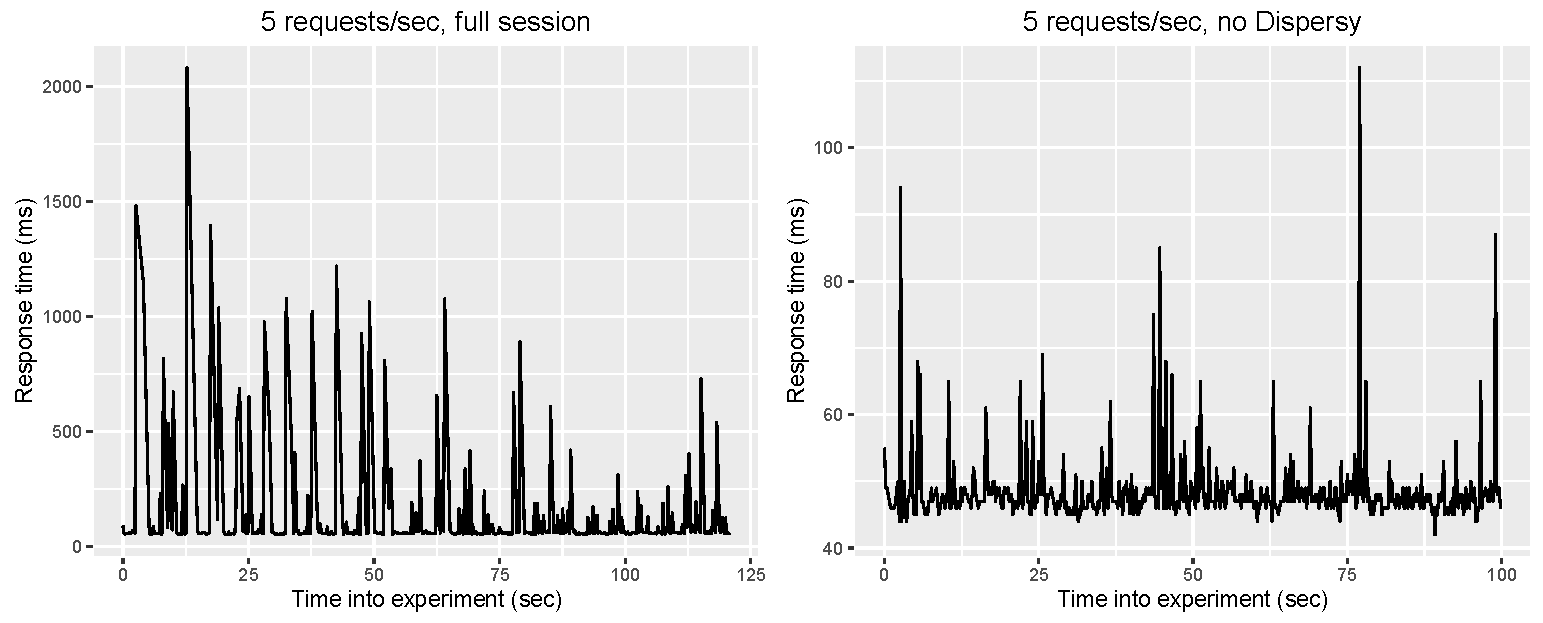
\includegraphics[width=1.0\columnwidth]{images/experiments/request_times_comparison}
	\caption{The response times of API requests, in a Tribler session both with Dispersy enabled and disabled.}
	\label{fig:api-performance}
\end{figure}

In the left plot, the response times of the performed requests with a regular Tribler session is displayed (corresponding to the 5 requests/sec row in Table \ref{table:performance-api-results} ) whereas in the right plot, we display the response times of the run with a disabled Dispersy. Note the different scale on the vertical axis, indicating that the requests performed when Dispersy is disabled, are substantially faster. Indeed, the average request time of the right plot in Figure \ref{fig:api-performance} is 48 milliseconds, significantly lower than the average of the response times when Dispersy is enabled, namely 123 milliseconds. While both plots are showing a spiky pattern, the standard deviation of the right plot is 5.73 milliseconds and the standard deviation in the left plot is 210.23 milliseconds. We conclude that the variation in response times is much lower in the right plot and that DIspersy is producing a huge amount of work, introducing considerable amounts of latency when performing API requests.\\\\
We identified a key issue here: the latency of methods to be processed in Twisted is high, causing the processing of incoming requests to be delayed. This is not only a situation that occurs in the REST API: the same situation holds for Dispersy and the tunnel community where possibly many incoming connections have to be processed and served. A step in the right direction is to make sure that there are no big blocking calls scheduled in Twisted that are considerable amount of time to complete. When a method with a long execution time is executed, Tribler is unable to process other events during that period, leading to a less responsive system. Ongoing work is focussed on making the disk operations in Tribler non-blocking. This should reduce the latency of event processing and improve the responsiveness of the system in general.\\\\
Table \ref{table:performance-api-results} provides us with another interesting observation, namely that it appears that the bandwidth is reducing as the number of requests per second increases. This becomes more obvious if we plot the theoretical maximum bandwidth together with the observed bandwidth during the experiments, see Figure \ref{fig:api-bandwidth-performance}. In this Figure, we presented both the obtained bandwidth by running a regular Tribler session and one where Dispersy has been disabled. We assume that each request contains 613KB (627.712 bytes) of data in the response body. The theoretical maximum obtainable bandwidth is determined as $ b = 613 * n $ where $ n $ is the number of requests per second and $ b $ is the theoretical maximum bandwidth in KB/s. In practice, we will never reach this theoretical bandwidth since some time is required to initialize the HTTP connection in Tribler which we do not consider in our simple model. Figure \ref{fig:api-bandwidth-performance} clearly shows the impact of a running Dispersy on the bandwidth. Whereas we almost obtain the theoretical bandwidth when we disable Dispersy, the gap between the theoretical maximum and observed bandwidths becomes bigger in the run where we use a full session. When performing fifteen requests per second, the bandwidth even decreases, possibly due to the high system load.\\

\begin{figure}[h!]
	\centering
	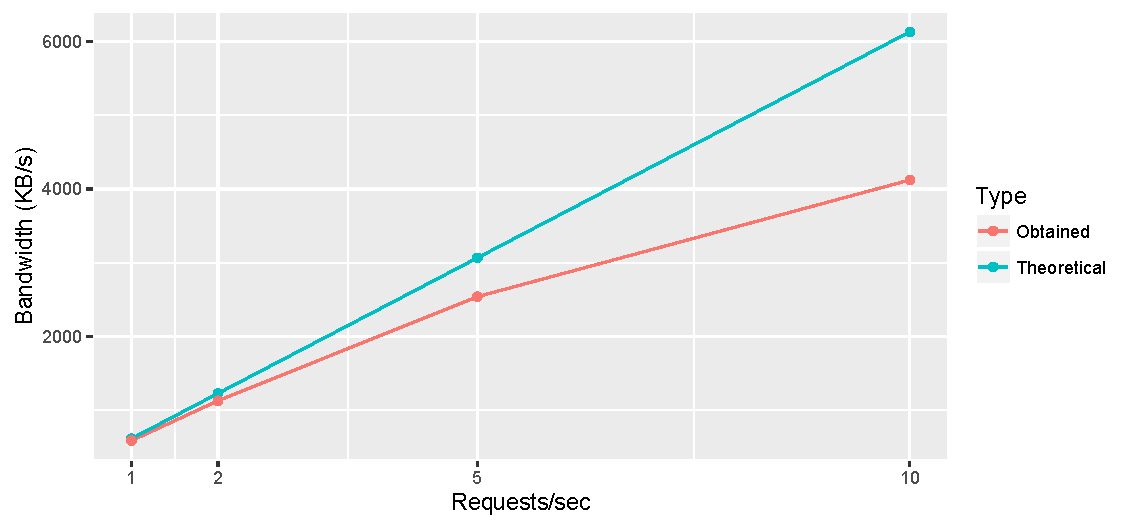
\includegraphics[width=1.0\columnwidth]{images/experiments/api_bandwidth_performance}
	\caption{The theoretical maximum bandwidth compared to the observed bandwidth in the experiments (using a full Tribler session and disabled Dispersy).}
	\label{fig:api-bandwidth-performance}
\end{figure}

We conclude this experiment with the argumentation that we can use the API response times as a benchmarking tool to measure the responsiveness of the Tribler core. Using the Apache JMeter application, we can easily build a stress test and verify whether performance has increased or decreased after a specific set of modifications. Implementation of a performance regression framework is considered future work. 

\section{Start-up Experience}
The first interaction with Tribler, is the process of booting the software. During this boot process, various operations are performed:
\begin{itemize}
	\item The Tribler state directory where runtime data are stored, is created and initialized with necessary files such as the SQLite database, the Dispersy member key pair and various configuration files.
	\item A connection to the persistent SQLite database is opened and initialized.
	\item Dispersy is initialized and the communities that are enabled in the configuration file are loaded.
	\item Various Tribler components are created, including the video streaming server, the RESTful API, the remote torrent handler, responsible for fetching torrent information from other peers and the \emph{leveldb} store, a key-value storage for torrent meta info.
\end{itemize}
The start-up process of the Tribler core proceeds sequentially and no parallel operations are implemented to speed up the process. Depending on the number of enabled components, the start-up time might vary.\\\\
To analyse the start-up time, we start Tribler 50 times in a row. The experiments are performed multiple times where in one experiment, the software is started for the first time, with no prior existing state directory. When starting Tribler with no prior existing state directory, a new one is created and the required files are initialized. In the other runs, a pre-filled database containing just over 100.000 torrents is used. This database is built by running Tribler idle for several hours, after subscribing to some popular channels to synchronize and discover as much torrents as possible. In both scenarios, there are no active downloads. A timer is started when the \emph{start} method of the \emph{Session} object is called and stopped when the notification that Tribler has started, is observed, allowing us to determine the total start-up time to a granularity of milliseconds. During the span of this thesis, there have been various changes to the start-up procedure of Tribler where code has been modified, removed and added. Since we would like to guarantee that our modifications do not significantly decrease the start-up speed and we make a comparison between the Tribler code in November '15 and July '16. The results are presented in Figure \ref{fig:startup_experiment}, where for each commit we compare, we present an empirical cumulative distribution function (ECDF) with the boot time in seconds on the horizontal axis and within each plot, the distribution of start-up times from a clean and pre-filled state directory.\\

\begin{figure}[!h]
	\centering
	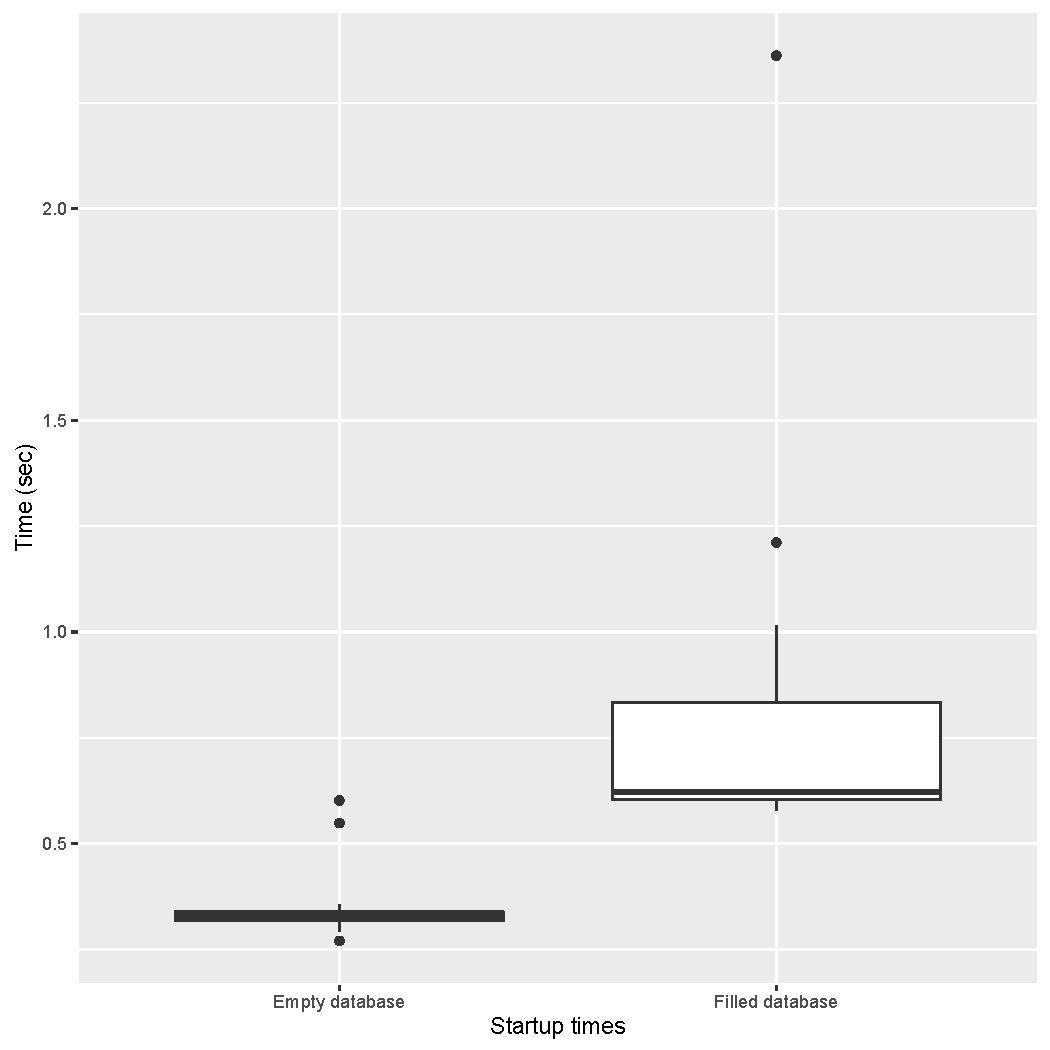
\includegraphics[width=1.0\columnwidth]{images/experiments/startup}
	\caption{The start-up time of Tribler from a clean and pre-filled state using the code base in November '15 and July '16.}
	\label{fig:startup_experiment}
\end{figure}

In both plots, It is clear that size of the Tribler database has impact on the time for Tribler to completely start. However, this impact is relatively minor since the system still starts within a second. We think that this statistic justifies removal of the splash screen that is shown in the old user interface: the relatively short time the splash screen would be visible in the new interface is so small that users would not even be able to read and interpret the content of the splash screen. In contrast to the old user interface, the new GUI starts Tribler and shows a loading screen after the interface has started. However, the difference is that users are able to already perform some actions before Tribler has started, such as the browsing of discovered content.\\\\
Whereas the boot times of the experiments performed with the November '15 code are very constant, we notice a larger variation in the runs with the code base from July '16, indicating that there is a component that has a high variation in initialization time during the start-up procedure. Further analysis learns us that this variation can be addressed to Dispersy, possibly caused by the initialization of one of the communities. However, further analysis of the boot time of Dispersy is outside the scope of this thesis work.

\section{Remote Content Search}
\label{sec:remote-content-search-experiment}
We wish to serve relevant information to users as fast as possible. To help users discover content they like, a remote keyword search has been implemented, allowing users to search for torrents and channels. Channel results are fetched by a query in the \emph{AllChannel} community whereas torrent results are retrieved by a query in the \emph{Search} community, however, for the experiments in this Section, we will focus on remote search for torrents since the amount of channels is rather small compared to the number of torrents available in the network.\\\\
Several experiments to verify the speed of a remote torrent search are discussed in this Section. A list of 100 search terms that have a high chance of triggering search results is used and each query is executed when there are at least twenty connected peers available in the \emph{Search} community (this condition is checked every second). The time-out period of the remote search is 60 seconds, indicating that incoming search results after this period are not regarded. This experiment is focussed on two performance statistics: the time interval until the first remote torrent search result comes in and the turnaround time of the search request, meaning the interval until the last search response arrives. We should note that users performing a remote search might see results earlier since a lookup query in the local database is performed in parallel (the performance of local search is discussed in Section \ref{sec:local-content-search}). The results of our experiment are visible in Figure \ref{fig:remote_search} where we created two ECDF plots with the distributions of time until the first response and time until the last response. On the horizontal axis, the measured time interval in seconds is visible.\\\\
Overall, the remote torrent search as implemented in Tribler is fast and performs reasonable. On average, there are 61 incoming search results for each performed query where the first torrent result takes on average 0.26 seconds to arrive. As we see in Figure \ref{fig:remote_search}, over 90\% of the first search results are available within a second. During our experiment, we always have the first incoming torrent result within 3.5 seconds. The plot displayed on the right shows the turnaround time of the request, indicating the time until the last response within our time-out period. On average, it takes 2.1 seconds for all torrent search results to arrive. In the plot, we see that in over 90\% of the search queries, we have all results within 10 seconds.\\

\begin{figure}[!h]
	\centering
	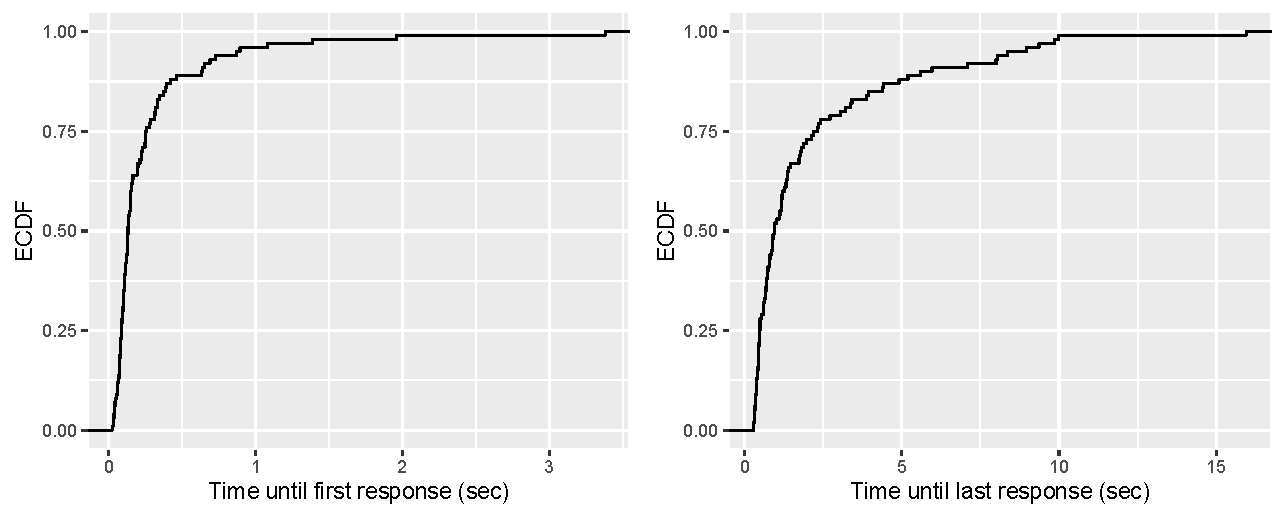
\includegraphics[width=1.0\columnwidth]{images/experiments/cdf_remote_search}
	\caption{The performance of remote content search, expressed in the time until the first response and time until last response.}
	\label{fig:remote_search}
\end{figure}

The same experiment has been performed in 2009 by Nitin et al. where 332 remote search queries have been performed. Their results are also presented in an ECDF in Figure \ref{fig:nitin_remote_search} where the time until the first response from any remote peer in the network is measured. The graph makes a comparison before and after a significant improvement to the input/output mechanism, causing messages to be exchanged at a faster rate. The observed average time until first response in 2009 is 0.81 seconds whereas the observed average time in our experiments is 0.26 seconds, more than three times as fast.

\begin{figure}[!h]
	\centering
	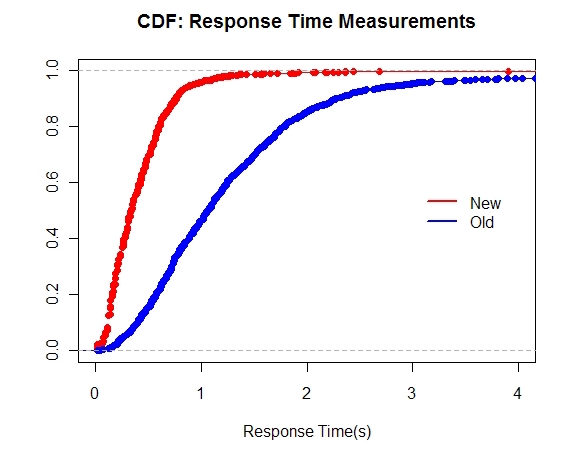
\includegraphics[width=0.7\columnwidth]{images/experiments/nitin_remote_search}
	\caption{The performance of remote content search, performed by Nitin et al. in 2009. The new remote search had an improved input/output mechanism, causing messages to be exchanged faster.}
	\label{fig:nitin_remote_search}
\end{figure}

\section{Local Content Search}
\label{sec:local-content-search}
In the previous Section, we demonstrated and elaborated the performance of the remote content search mechanism. Now, we will shift the focus to performance measurements of local content search, which is considered more trivial than the remote search counterpart due to the lack of network communication. In particular, our goal is to quantify the performance gain or loss when switching to the new relevance ranking algorithm that uses a newer search engine, as described in Chapter \ref{sec:relevance-ranking-algorithm}.\\\\
The set-up of this experiment is as follows: a database with just over 100.000 torrents is used. Around ten seconds after starting Tribler, we perform a local torrent search every second and we do this for 1.000 random keywords that are guaranteed to match at least one torrent in our database. We will measure both the time spent by the database lookup and the time it takes for the data to be post-processed after being retrieved from the database.. In the code used in November '15, this post-processing step involves determining the associated channels that are containing a specific torrent result. This experiment is performed for the old method that uses the \emph{Full Text Search 3 (FTS3)} engine and the new procedure that uses the more recent \emph{Full Text Search 4 (FTS4)} engine. According to the SQLite documentation, FTS3 and FTS4 are nearly identical, however, FTS4 contains an optimization where results are returned faster when performing searches with keywords that are common in the database. The results of the experiments with the old and new local search logic are visible in Figure \ref{fig:local-search-fts3-fts4}, presented in two ECDF plots with on the horizontal axis, the time of either the database query time (the red line) and the total time for the processing of results, including the query time (the blue/green line).\\

\begin{figure}[h!]
	\centering
	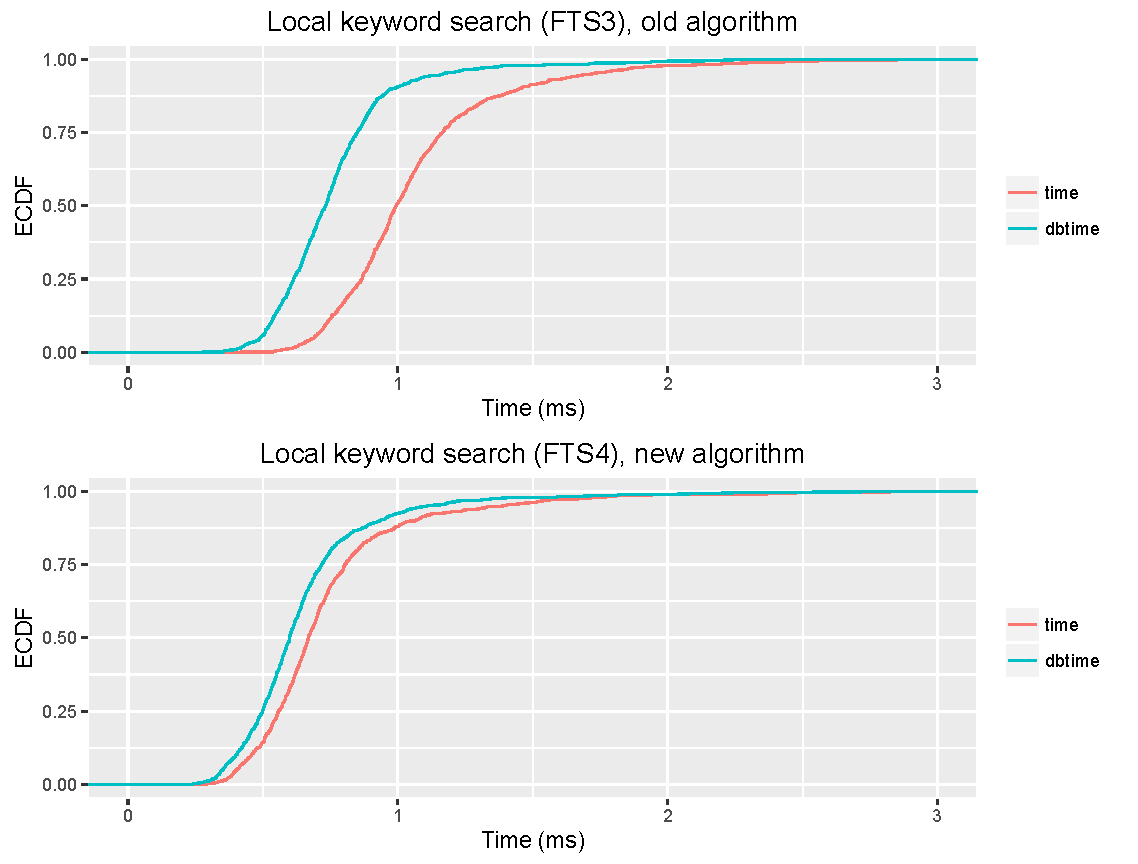
\includegraphics[width=1.0\columnwidth]{images/experiments/local_search_fts3_fts4}
	\caption{A comparison of the performance of local keyword searches between the old local search mechanism utilizing the FTS3 and FTS4 engine.}
	\label{fig:local-search-fts3-fts4}
\end{figure}

Local content search is very fast, delivering results in several milliseconds and low priority should be given to performance engineering on the local content search engine. We see that the two lines in the FTS3 and FTS4 plots have moved closer to each other which means that the total time of post-processing of torrent results has decreased. This is in line with our expectations since the new relevance ranking algorithm should be less computationally expensive than the old one. In addition, the new algorithm takes less factors in considering, for instance, the swarm health of the torrent. The increase in performance from FTS3 to FTS4 is visible but not very significant.\\\\
In 2009, Nitin et al. performed the same experiment where they used a database filled with 50.000 torrents. Their generated ECDF is displayed in Figure \ref{fig:local-search-nitin}. We notice that the performance of local search in our experiment is dramatically better than the performance obtained during the 2009 experiment. This can be explained by the fact that Tribler used a custom inverted index implementation when the experiment in 2009 was conducted. An inverted index is a data structure where a mapping is stored from words to their location in the database and is used on a large scale by search engines, including the FTS engine of SQLite. By utilizing this mapping when performing a full text search, we can get results in constant time. However, there is a slight overhead for maintaining and building the inverted index when new entries are added to the database, also impacting the size of the database disk file. The built-in FTS engine of SQLite is optimized to a large extent and clearly offers a higher performance than a custom implementation.

\begin{figure}[h!]
	\centering
	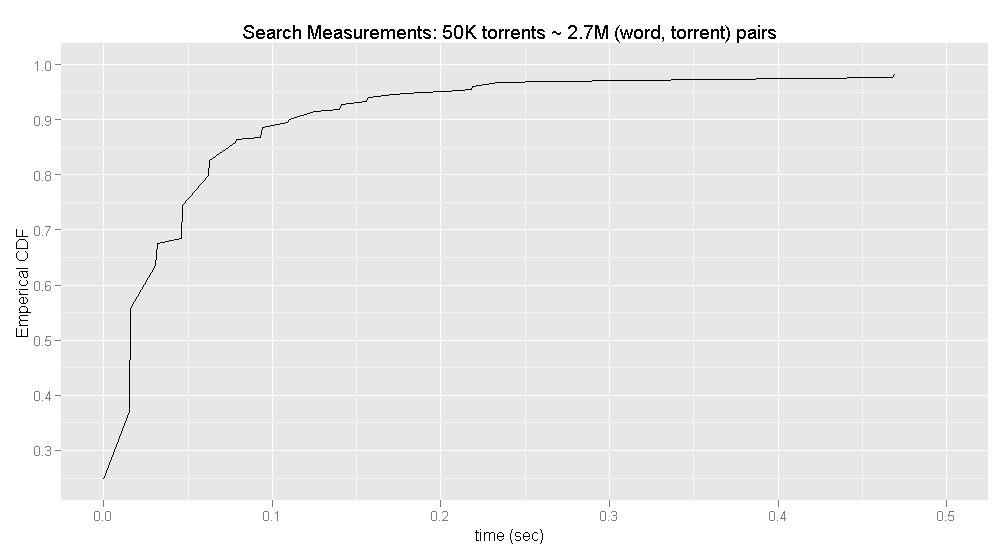
\includegraphics[width=1.0\columnwidth]{images/experiments/nitin_local_search}
	\caption{The performance of a local database query as verified by Nitin et al. in 2009.}
	\label{fig:local-search-nitin}
\end{figure}

\section{Video Streaming}
The embedded video player in Tribler allows users to watch a video that is being downloaded and the working is explained in more detail in Chapter \ref{subsubsec:video-server}. Video playback has been available since Tribler 4.0 and is implemented using the VLC library. One distinguishable feature is support for seeking so the user can jump to a specified time offset in the video. Video downloads have a special \emph{video on demand (VOD)} mode which means that the libtorrent piece picking mechanism uses a linear policy mode. In this mode, pieces are downloaded in a sequential order. When the user seeks to a position in the video, the prioritization of the pieces is modified, giving priority to pieces just after the specified seek position. Users also have the possibility to use an external video player that support playback of HTTP video streams.\\\\
The bytes are streamed to a VLC-compatible client using a HTTP stream. When Tribler starts, a video server is started if enabled in the configuration file. This server supports HTTP range requests which means that a specific part of a video file can be queried by using the HTTP \emph{range} header. This is useful when the user performs a seeking operation since only a specific part of the file has to be returned in the HTTP response, possibly saving a huge amount of bandwidth. If some requested pieces are not available, the video server will wait until these bytes are downloaded before returning these bytes in the response.\\\\
To improve user experience, we wish to minimize the delay that users experience when performing a seek operation in the video player. The experiment performed in this Section, will quantify this buffering delay. For this purpose, the well-seeded \emph{Big Buck Bunny}\footnote{https://peach.blender.org} movie will be downloaded. The movie file has a size of 885.6 MB and has a duration of 9 minutes and 56 seconds. We will perform various HTTP range requests using the \emph{curl} command line tool\footnote{https://curl.haxx.se}, immediately after starting the download in Tribler. For every run, we will request 10 megabyte of data and we will measure the total time it takes for each HTTP request to complete. The results are visible Table \ref{table:video_player_seek_times} where we specified the first requested byte and the time until the request has been fulfilled and the response is received.\\

\begin{table}[]
	\centering
	\begin{tabular}{|l|l|}
		\hline
		First byte               & Time until request done (sec) \\ \hline
		0                        & 11.6                  \\ \hline
		$ 1 * 10^9 $ & 64.4                  \\ \hline
		$ 2 * 10^9 $ & 64.6                  \\ \hline
		$ 3 * 10^9 $ & 65.9                   \\ \hline
		$ 4 * 10^9 $ & 100.6                   \\ \hline
		$ 5 * 10^9 $ & 115.6                   \\ \hline
		$ 6 * 10^9 $ & 115.8                  \\ \hline
		$ 7 * 10^9 $ & 12.2                  \\ \hline
		$ 8 * 10^9 $ & 66.6                   \\ \hline
		$ 9 * 10^9 $ & 52.4                   \\ \hline
	\end{tabular}
	\caption{Performance of the video server when requesting bytes at different offsets of the video being downloaded.}
	\label{table:video_player_seek_times}
\end{table}

Theoretically, we would expect around the same request time for each range request, assuming that the availability of each piece is high. When performing a seek operation in the video, the piece picking mechanism adjusts priorities and these prioritized pieces should start to download immediately. The experiments shows various anomalies in this mechanism where it might take up to two minutes for data to be available. Further investigation of this issue learns us that the video player always tries to download the first 10\% of the video file. We found out that this is intended behaviour of the code since VLC needs the information embedded in the file header first. This file header provides information about the file type, file duration and encoding used. There are some video formats where this kind of information is present at the end of the video file.\todo{conclusie??}\\\\

\section{Content Discovery}
\label{sec:content-discovery}
Content discovery is a key feature of Tribler. By running Tribler idle for a while, content is synchronized with other peers using the Dispersy messaging mechanism. When a user starts Tribler for the first time, there is no discovered content yet. We will verify the discovery speed of content after a first fresh start. The experiment is structured as follows: we measure the interval from the completion of start procedure to the moment in time where the first content is discovered. We perform these experiments for both torrents and channels and repeat this fifteen times. The results are visible in Figure \ref{fig:content_discovery_speed} where we created an ECDF with a distribution summary of the discovery times of torrents (green line) and channels (orange line).\\

\begin{figure}[!h]
	\centering
	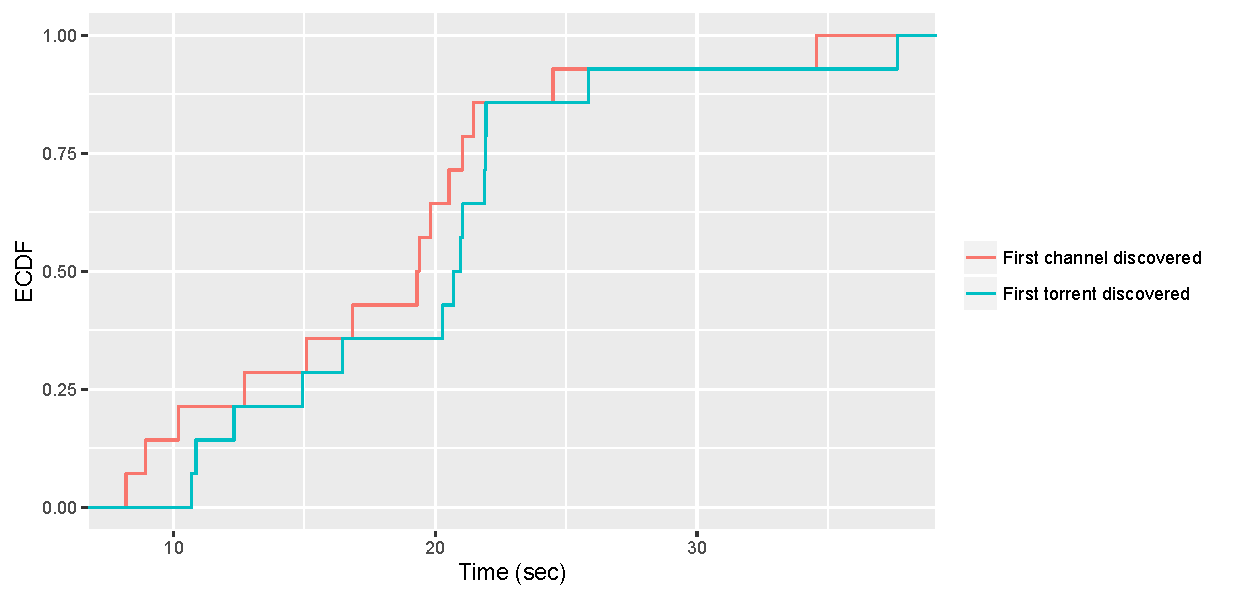
\includegraphics[width=1.0\columnwidth]{images/experiments/content_discovery}
	\caption{The discovery time of the first channel and torrent after starting first starting Tribler.}
	\label{fig:content_discovery_speed}
\end{figure}

The delay of discovering the first channel is reasonably: this happens on average 18 seconds after start-up. In all runs, we have our first channel discovered within 35 seconds after Tribler starts. Discovery times of the first torrent is slightly slower and in all runs, the first torrent in a channel is discovered within 40 seconds. Figure \ref{fig:content_discovery_speed} suggests that a torrent discovery always happens after there is at least one discovered channel. This is true: after the channel is discovered, the \emph{PreviewChannel} community is joined where torrents are exchanged and discovered after a while.\\\\
In the old user interface, users were presented with a blank screen with no feedback about content that is being discovered in the background. In the new interface, the user is presented with a screen that informs the user that Tribler is discovering the first content. This screen is only shown the first time Tribler is started and is dismissed when there are five discovered channels after which the page with an overview of discovered channels is presented to the user.

\section{Channel Subscription}
When Tribler runs idle, not all available content in the network is discovered. The majority of content is discovered when users subscribe to a channel (in the old user interface, this is referenced to as marking a channel as favourite). When Tribler discovers a new channel, users are able to browse a preview of this channel. Internally, Tribler connects to the \emph{PreviewChannelCommunity} associated with that channel, a community derived from the \emph{ChannelCommunity}. In this preview community, the amount of torrents that are collected is limited. The \emph{ChannelCommunity} is joined the moment the user subscribes to a channel, after which the full range of content is synchronized. Removing the preview mechanism might significantly increases the resource usage of the Tribler session since the amount of incoming messages to be decoded and verified will increment.\\\\
The experiment as described in this Section, will focus on the discovery speed of additional content after the user subscribes to a specific channel and on the resource allocation when we are running Tribler without enabling a preview mechanism of channels. For the first experiment where we determine the discovery speed of additional content inside a channel, the twenty most popular channels (having the most subscribers) are determined. To get these channels, we have used a Tribler state directory with many discovered channels but void of any channel subscriptions. Exactly ten seconds after Tribler started, we subscribe to one of these popular channels and we measure the time interval between subscription to the channel and discovery of the first additional torrent in this channel. Tribler is restarted between every run and the state directory is cleaned so we guarantee a clean state of the system. The observed results are visible in Figure \ref{fig:channel-subscription}.

\begin{figure}[!h]
	\centering
	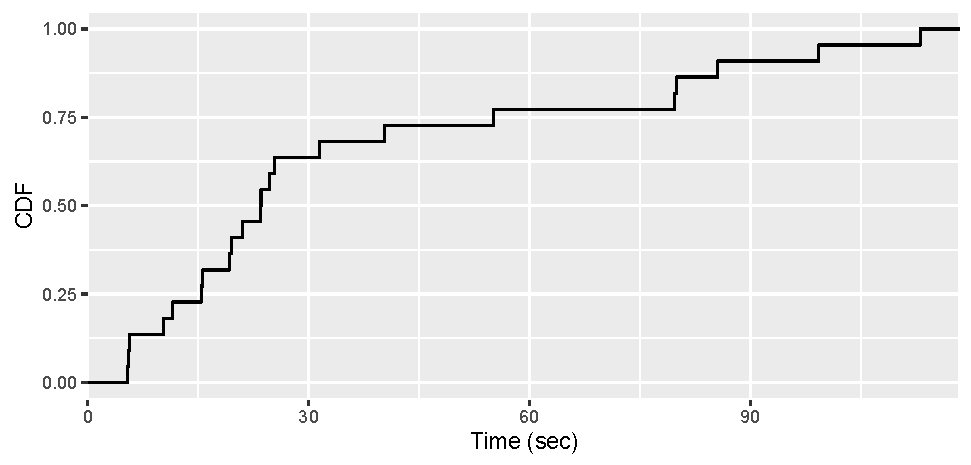
\includegraphics[width=1.0\columnwidth]{images/experiments/channel_subscription}
	\caption{An ECDF of discovery times of the first additional torrent after subscribing to a popular channel.}
	\label{fig:channel-subscription}
\end{figure}

The average discovery time of additional torrents after subscription to a channel is 36.8 seconds which is quite long, compared to the discovery speed of the first channel and torrent as described in Section \ref{sec:content-discovery}. The discovery times have a high variation as can be seen in Figure \ref{fig:channel-subscription}. This can be explained by the fact that immediately after subscribing to a channel, Tribler will connect to the \emph{ChannelCommunity} that is joined after subscription and peers have to be found.\\\\
To verify the impact of automatically subscribing to each channel when it is discovered, we perform a CPU usage measurement. In two idle runs of a Tribler session, both lasting for ten minutes, we measure the CPU usage every ten seconds using output provided by the \emph{top} tool. In the first run, a regular Tribler session is used where previews of discovered channels are enabled. In the second run, we bypass the preview of a discovered channel and immediately join the channel, synchronizing all available content. Both types of runs start with an empty state directory. The results of this experiment are visible in Figure \ref{fig:channel-subscription-cpu}.

\begin{figure}[!h]
	\centering
	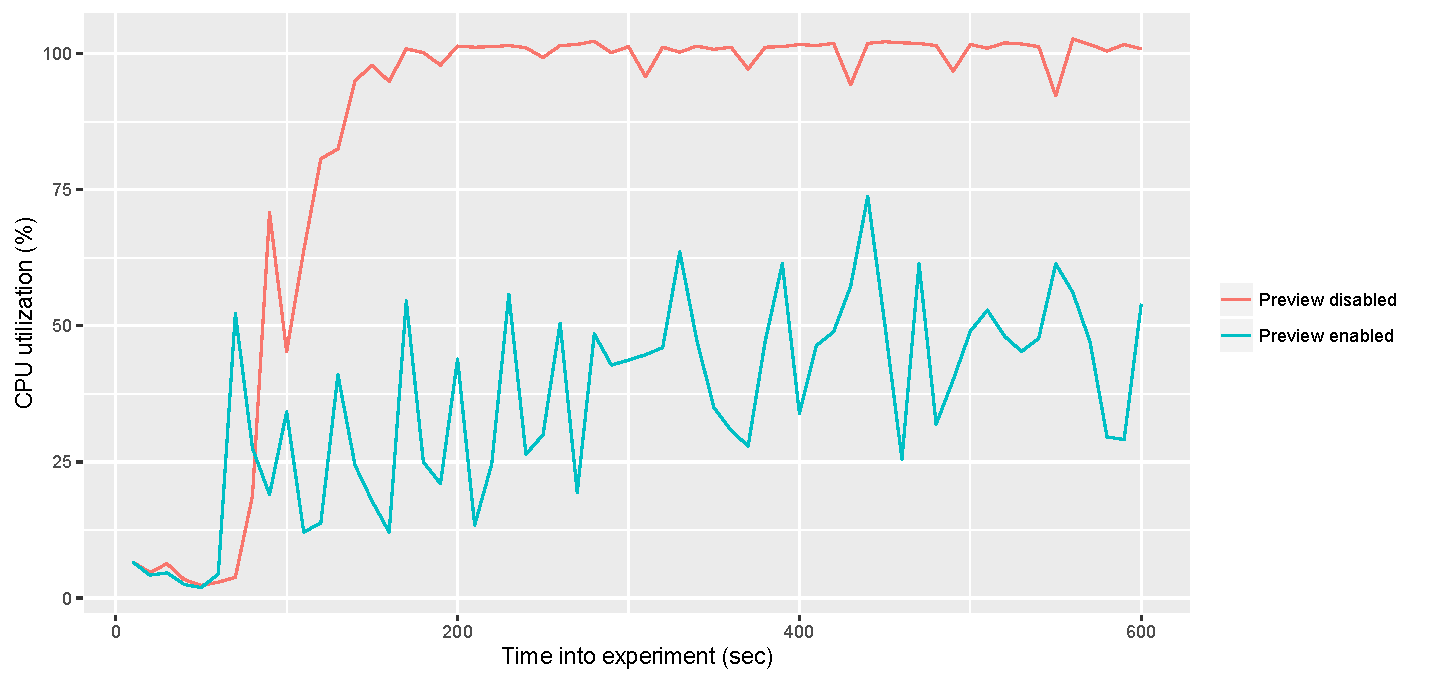
\includegraphics[width=1.0\columnwidth]{images/experiments/subscribe_cpu_experiment}
	\caption{The CPU utilization of one core during a period of ten minutes with channel preview enabled and disabled.}
	\label{fig:channel-subscription-cpu}
\end{figure}

Whereas the CPU usage of the normal run is around 45\% on average, the CPU is quickly rising to 100\% utilization when we enable the auto-join mechanism of channels. This shows that it is infeasible to enable this auto-join feature if we still wish to guarantee a responsive system. One might limit the rate at which discovered torrents are fetched, however, this requires a feedback mechanism where we should notify other peers in the community to limit the amount of messages sent to the peer that is discovering content. Implementing of such as feature is outside the scope of this thesis work and is considered future work.

\section{Torrent Availability and Lookup Performance}
While specific information about torrents such as the name and file names are distributed within the Dispersy communities, this does not hold for the meta info about the torrent itself, which includes additional data such as available trackers and information about pieces. This meta info might be important for users since trackers provides information about the health of a torrent swarm. The experiments as explained in this Section, will investigate the torrent availability and lookup performance of meta info of torrents, either by using downloading them from remote peers in the Tribler network or from the \emph{Distributed Hash Table (DHT)}.

\subsection{Trivial File Transfer Protocol Handler}
When users are performing a remote torrent search, the first three incoming results are pre-fetched in the old user interface which means that the meta info of these torrents are fetched automatically. An incoming search result might contain information about remote peers (candidates) that have meta info of this torrent available. If candidates for a specific remote torrent result are present, an attempt to fetch the torrent meta info from this candidate is scheduled. This request is performed using the \emph{Trivial File Transfer Protocol (TFTP)}\cite{sollins1992tftp} which is a simplified version of the more sophisticated \emph{File Transfer Protocol (FTP)}\cite{postel1985rfc}, commonly used to transfer files over the internet. TFTP is also used to transfer meta data about torrent files such as thumbnails between peers, however, meta data of torrents is currently disabled in Tribler. The implementation of TFTP is located in the core package of the code base.\\\\
There has been no published studies yet about the performance of our TFTP implementation so we have no available reference material. The experiment performed in this Subsection will focus on the performance of TFTP when fetching meta info from remote peers. We start from a clean state directory and exactly one minute after starting Tribler, we perform a remote torrent search. For each incoming remote search result, we perform a TFTP request for each candidate attached to this result. We perform ten remote torrent search operations, with interval of 60 seconds between them. For every incoming result, we schedule a remote torrent lookup. After eleven minutes, we stop Tribler and gather the statistics of the TFTP sessions. The observed results are visible in Table \ref{table:tftp-performance}.\\

\begin{table}[h!]
	\centering
	\begin{tabular}{|l|l|}
		\hline
		\emph{Total requests scheduled} & 1008 \\ \hline
		\emph{Requests in queue} & 761 (75.5\%)\\ \hline
		\emph{Requests failed} & 106 (10.5\%)\\ \hline
		\emph{Requests succeeded} & 141 (14.0\%)\\ \hline
	\end{tabular}
	\caption{A breakdown of the performed requests during the TFTP performance measurement.}
	\label{table:tftp-performance}
\end{table}

We notice that the queue keeps growing: when our experiment is finished, 75.5\% of the initiated requests is still in the queue. The second observation is the high failure rate, when compared to the amount of succeeded requests (42.9\% if we do not consider the requests in the queue). We identified two underlying reasons for the failed requests. First, some of the requests timed out, possibly due to the fact that various remote peers are not connectible. A solution for this kind of failure would be a robust NAT puncturing method. The second reason is that the remote peer might not have the requested file in the local persistent storage. While this situation might seem unusual, it can happen if the remote peer has the requested torrent in the SQLite database but not in the meta info store, a separate persistent database. We can solve this by not returning this peer as candidate if the torrent is not available in the meta info store. This solution will also reduce the total bandwidth used by the TFTP component.\\\\
Next, we will focus on the turnaround time of successful TFTP requests, presented in the ECDF in Figure \ref{fig:tftp_performance-success}. Here, we notice the weird distribution of the turnaround times: we would expect that the total request times to fetch meta info using TFTP is somewhat constant, however, we see outgoing requests that take over 400 seconds to complete. This trend will probably continue if we did not stop the experiment after eleven minutes. The most reasonable explanation for this is that requests are added to the request queue at a faster rate than the processing speed of these requests. This also explains the values denoted in Table \ref{table:tftp-performance} where 75.5\% of the request are still in the queue after the experiment ends. Better support for parallel requests should help, however, this is considered further work.

\begin{figure}[!h]
	\centering
	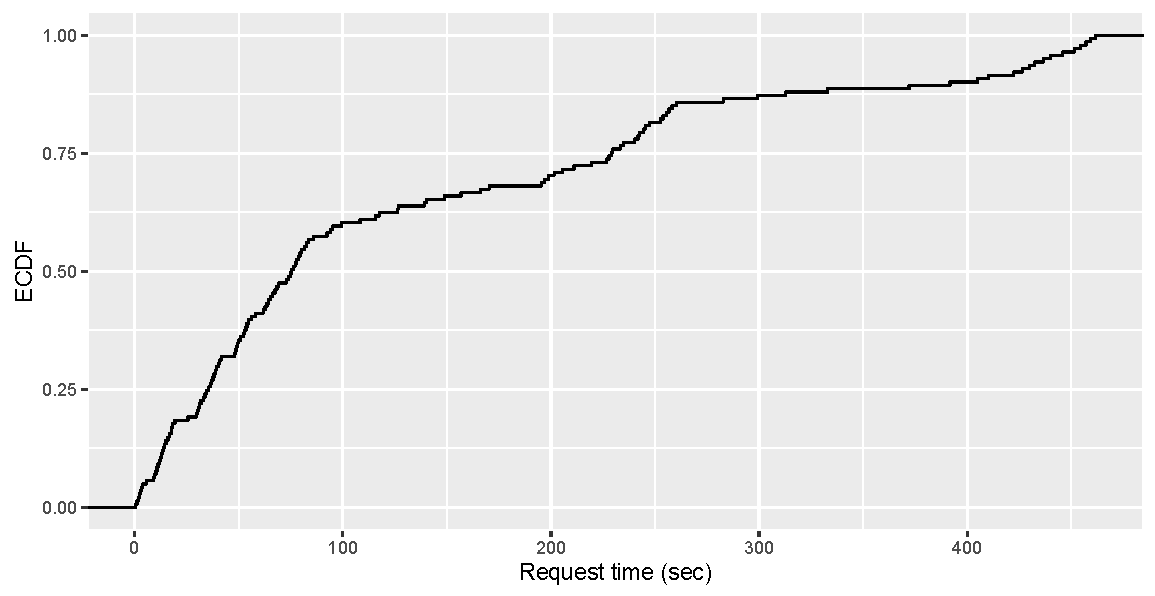
\includegraphics[width=0.9\columnwidth]{images/experiments/tftp_performance}
	\caption{An ECDF of the performance of the torrent meta info download mechanism using TFTP in Tribler.}
	\label{fig:tftp-performance-success}
\end{figure}

\subsection{Distributed Hash Table}
Another source of torrent meta info is the DHT. In the DHT we can lookup meta info of a torrent, identified by an infohash by invoking the \emph{download\_torrentfile} in the \emph{Session} object. In this Section, we will perform an experiment to get insights in the availability of torrent files and the performance of lookup operations in the DHT. This experiment is relevant to the user experience since users that want to determine whether specific content is interesting or not, they first might want to view meta info of the torrent file, including names and sizes of the files the torrent contains. This meta info should be available as soon as possible.\\\\
In the old wxPython user interface, the torrent file is fetched when the user single clicks on a torrent in a list of torrents, either when browsing through contents of a channel or after performing a remote keyword search. In addition, when executing a remote search, the first three top-results are pre-fetched since there is a higher probability that the user might be interested in them. For this experiment, a popular channel with over 5.000 torrents is considered and a subset of 1.000 torrent infohashes in this channel is determined. We start Tribler from a clean state and every 40 seconds, a DHT query is performed with one of the 1.000 random infohashes. The time-out period used in Tribler is 30 seconds, after which a failure callback is invoked and an error is displayed in the user interface to notify the user about the failed request. The results of this experiments are visible in the ECDF depicted in Figure \ref{fig:metainfo_fetch}.\\

\begin{figure}[!h]
	\centering
	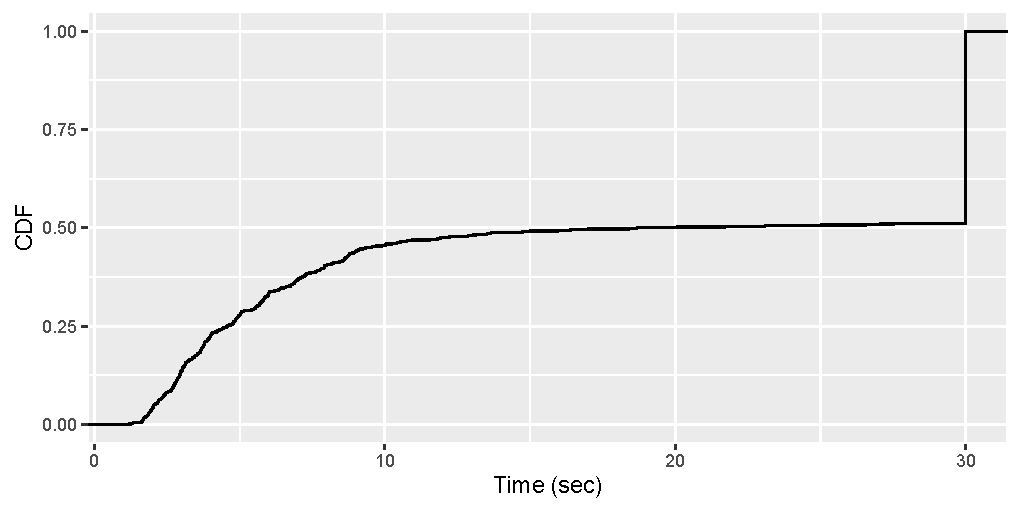
\includegraphics[width=1.0\columnwidth]{images/experiments/metainfo_fetch}
	\caption{Test.}
	\label{fig:metainfo_fetch}
\end{figure}

We immediately notice that the failure rate of DHT lookups is quite high: a little under 50\% of the lookup operations are timing out and never succeed. This issue might be addressed to dead torrents (when no peers in the DHT have this torrent information available) or private torrents (torrents which information is not exposed in the DHT). The amount of failures might be even higher in a less popular channel since the content in these channels are probable to be less seeded. As explained in the previous Subsection, the DHT is not the only source for torrents in Tribler and we might also fetch torrents from other peers using TFTP. Unfortunately, the approach of fetching meta info about torrents from other peers is only usable when searching for torrents. Caching and exchanging torrent candidates is not successful since the availability of candidates cannot be guaranteed.\\\\
The average lookup time of torrents that are successfully fetched from the DHT is 5.81 seconds which is reasonably fast. Additionally, Figure \ref{fig:metainfo_fetch} shows that a little over 90\% of the successfully fetched torrents are retrieved within 10 seconds.\\\\
To improve performance of meta info lookups, dead torrents should be handled correctly. One possible solution might be an implementation of a periodical check for each incoming torrent. By limiting the number of outstanding DHT requests, this approach does not create require much additional resources. To further improve performance, the result of DHT lookups might be disseminated to remote peers in the network. Torrents that are not successfully fetched from the DHT, could be hidden automatically in the user interface. The downside of this approach is that it might not give a realistic view of the availability of a torrent since their might be candidates which have a copy of this torrent available.
\chapter{Conclusions}
\label{chapter:conclusions}

% Tribler needs a culture change, this work tries to transform the way Tribler development is conducted...
The work in this thesis investigates the technical debt that has been accumulated by over 40 unique contributors over the last ten years of scientific research in the area of decentralized networks. After a comprehensive discussion of the architectural evolution Tribler has made, A future-proof and robust architecture of Tribler is proposed, discussed and some parts of the new design have been implemented. The main components as created in this thesis are a new user interface, built using the Qt framework, and a REST API, allowing Tribler to run on remote devices while giving developers high amounts of flexibility and ease when developing with Tribler. The testing environment has been improved with the addition of proper and stable unit tests and the tests are now executed on multiple platforms, allowing us to find defects due to platform incompatibilities earlier in the development process. Summarizing, this work transformed Tribler from an unattractive, unmaintained and untested system into a platform that is ready for development during the next decade of scientific research.\\\\
While this is a step in the right direction, there still is a lot of work to do by the next generation of Tribler developers. We should learn from the mistakes made in the past years. Being critical towards the implementation of quick workarounds is one example of that. Mandatory code reviews by other team members helps to improve one's code and to get a more critical attitude towards favouring short-term decisions over long-term agreements. We also propose that it is the responsibility of every developer to write code that is covered by the right amount of tests. By forcing a strict increasing code coverage policy, the code coverage metric can be controlled and gradually improved over time.\\\\
Additional future work proposed is the implementation of the trust walker, which will become the foundations of the Tribler platform. This way, the Dispersy framework could be removed, allowing the deletion of much legacy code. Although not the main subject of this thesis, the amount of accumulated debt in Dispersy is also rather high. From a performance perspective, research should be conducted to see how the performance on low-end embedded devices could be improved. Since our main performance bottleneck is the limited amount of CPU power in a specific core, one of the proposed solutions is to increase utilization of multi-core architectures. This can be achieved by splitting the architecture of Tribler in separate components that can independently run on several cores, however, this requires one to think very carefully about the final design and communication structure.

%% Use letters for the chapter numbers of the appendices.
\appendix

\chapter{Gumby scenario file commands}
As described in Chapter \ref{chapter:experiments}, a standalone Tribler runner that uses a scenario file has been created. The scenario file allows developers to specify commands at specific points in time after Tribler has booted. This Appendix describes the implemented commands and usage.

\begin{table}[h!]
	\begin{tabularx}{\textwidth}{|X|X|X|}
		\hline
		\textbf{Command} & \textbf{Argument(s)} & \textbf{Description}\\ \hline
		\emph{start\_session} & - & Start a Tribler session.\\ \hline
		\emph{stop\_session} & - & Stop a running Tribler session.\\ \hline
		\emph{stop} & - & Stop the experiment and write the gathered statistics.\\ \hline
		\emph{clean\_state\_dir} & - & Clean the default state directory of Tribler.\\ \hline
		\emph{search\_torrent} & The search query and optionally the minimum number of peers required in before the search is performed. & Perform a remote torrent search.\\ \hline
		\emph{local\_search\_torrent} & The search query. & Perform a local torrent search in the database.\\ \hline
		\emph{get\_metainfo} & The infohash of the torrent to be fetched. & Fetch meta info of a specified torrent from the DHT.\\ \hline
		\emph{start\_download} & The URI of the download. & Start a download from a torrent specified by a given URI.\\ \hline
		\emph{subscribe} & The Dispersy channel identifier of the channel (can also be \emph{random}). & Subscribe to a random or specified channel.\\ \hline
	\end{tabularx}
	\caption{An overview of commands for the Gumby scenario file when performing experiments with Tribler.}
	\label{table:gumby-scenario-file}
\end{table}

\bibliography{report}

\end{document}

